% Supplementary Information content. Compiled on its own by si.tex, and
% appended to the manuscript by combined.tex (via main.tex) for latexdiff.
% Edit the SI here; there is no other copy.

%%%%%%%%%%%%%%%% START OF SUPPLEMENT %%%%%%%%%%%%%%%

% Nature Communications style: display items restart at 1 and are labelled
% "Supplementary Figure 1" / "Supplementary Table 1"; text sections are
% "Supplementary Note 1" etc. Cite them as Supplementary Fig. / Table / Note N.
% Equations and pages keep the S prefix.
\renewcommand{\thefigure}{\arabic{figure}}
\renewcommand{\thetable}{\arabic{table}}
\renewcommand{\figurename}{Supplementary Figure}
\renewcommand{\tablename}{Supplementary Table}
\newcounter{supnote}
\newcommand{\supnote}[2]{\refstepcounter{supnote}\label{#2}\subsection*{Supplementary Note \thesupnote: #1}}
\renewcommand{\theequation}{S\arabic{equation}}
\renewcommand{\thepage}{S\arabic{page}}
\setcounter{figure}{0}
\setcounter{table}{0}
\setcounter{equation}{0}
\setcounter{page}{1} % not 0 as \newpage already started a supplementary page
% References continue the numbering from the main text.

% Restarting the counters above also restarts the names hyperref builds its PDF
% anchors from: those come from \theH<counter>, not from \the<counter>, so the
% S prefix added above does not reach them. Without these lines Fig. S16 asks
% for the anchor "figure.16" that main-text Fig. 16 already claimed, pdfTeX
% drops the duplicate, and the supplementary link lands on the main-text float
% carrying the same number. Nothing here is printed; it only names the targets.
\providecommand{\theHfigure}{\arabic{figure}}
\providecommand{\theHtable}{\arabic{table}}
\providecommand{\theHequation}{\arabic{equation}}
\renewcommand{\theHfigure}{S\arabic{figure}}
\renewcommand{\theHtable}{S\arabic{table}}
\renewcommand{\theHequation}{S\arabic{equation}}


%%%%%%%%%%%%%%%% SUPPLEMENT TITLE PAGE %%%%%%%%%%%%%%%

\begin{center}
\section*{Supplementary Materials for\\ Quantifying comprehensive marine vessel emissions using satellite data fusion}

% Plain text rather than \author, which belongs to the journal class's title
% page and is not used in the stand-alone SI
Gavin~McDonald$^{1,2,3,\ast}$,
Pol~Carbó-Mestre$^{1,2,3}$,
Olivier~Deschenes$^{3,4}$,
Jennifer~Bone$^{1,2,3}$,
E.~Fernando~Cagua$^{5}$,
Anna~Hughes$^{5}$,
David~Kroodsma$^{5}$,
Fernando~S.~Paolo$^{5}$,
Mark~Powell$^{5}$,
Zihan~Wei$^{5}$,
Christopher~Costello$^{1,2,3,4}$

\medskip
{\small
$^{1}$Marine Science Institute, University of California, Santa Barbara, CA 93106, USA\\
$^{2}$Bren School of Environmental Science \& Management, University of California, Santa Barbara, CA 93106, USA\\
$^{3}$Environmental Markets Lab, University of California, Santa Barbara, CA 93106, USA\\
$^{4}$Department of Economics, University of California, Santa Barbara, CA 93106, USA\\
$^{5}$Global Fishing Watch, Washington, DC 20036, USA\\[4pt]
$^{\ast}$Corresponding author. Email: gmcdonald@bren.ucsb.edu}
\end{center}

% The list of Supplementary items starts on page 2, as the journal asks
\newpage

\subsubsection*{This PDF file includes:}
\begin{itemize}
    \item Supplementary Figures 1 to 16
    \item Supplementary Tables 1 to 10
    \item Supplementary Notes 1 to 3
\end{itemize}

\subsubsection*{Other Supplementary Materials for this manuscript include the following:}
\begin{itemize}
    \item Supplementary Data 1 to 3 (CSV files; described below)
\end{itemize}

\subsubsection*{Supplementary Figures}
\begin{itemize}\setlength{\itemsep}{0pt}
    \item[1.] Fishing and non-fishing components of the global emissions time series and maps (p.~\pageref{fig:fig-spatial-temporal-richness-by-fleet-total-pseudolog})
    \item[2.] Spatial maps of 2025 emissions for each GHG and pollutant (p.~\pageref{fig:fig-pollutant-maps})
    \item[3.] Monthly global emissions time series for each GHG and pollutant (p.~\pageref{fig:fig-pollutant-time-series})
    \item[4.] CO$_{2}$ emissions by country and activity type for AIS-broadcasting vessels, 2025 (p.~\pageref{fig:fig-emissions-by-country-and-activity-type})
    \item[5.] Trend in CO$_{2}$ emissions by ocean, normalized to the 2017 baseline (p.~\pageref{fig:fig-emissions-marine-ocean-other})
    \item[6.] Annual CO$_{2}$ emissions by ocean and data source (p.~\pageref{fig:fig-annual-emissions-by-ocean-and-data-source})
    \item[7.] Passenger vessels by length bin, 2017 against 2025 (p.~\pageref{fig:figS-passenger-size-panels})
    \item[8.] Relative change since 2017 in fleet size, AIS messages and CO$_{2}$ emissions by vessel class (p.~\pageref{fig:figS-fleet-growth-by-year})
    \item[9.] Change in AIS-based CO$_{2}$ emissions since 2017 by vessel class family and length (p.~\pageref{fig:figS-growth-timeline-by-family-length})
    \item[10.] Fleet composition in 2025: share of the fleet against share of CO$_{2}$ by vessel class (p.~\pageref{fig:figS-fleet-sankey-with-series-2025})
    \item[11.] Annual CO$_{2}$ emissions, AIS messages and vessel counts by AIS receiver type (p.~\pageref{fig:fig-annual-emissions-by-ais-receiver-type})
    \item[12.] Annual CO$_{2}$ emissions by AIS receiver type for the ten highest-emitting flags (p.~\pageref{fig:fig-annual-emissions-by-ais-receiver-type-top-flags})
    \item[13.] Spatial change in CO$_{2}$ emissions between 2017 and 2025 by AIS receiver type (p.~\pageref{fig:fig-co2-emissions-change-map-by-receiver-type})
    \item[14.] Trends in our AIS-based and fused estimates against other inventories (p.~\pageref{fig:figS-inventory-comparison-all-sources})
    \item[15.] AIS carriage saturation by vessel size (p.~\pageref{fig:figS-ais-carriage-saturation-by-size})
    \item[16.] S1 detection density by length bin and AIS match status (p.~\pageref{fig:figS-density-by-match-status})
\end{itemize}

\subsubsection*{Supplementary Tables}
\begin{itemize}\setlength{\itemsep}{0pt}
    \item[1.] 2017 and 2025 emissions by data source and pollutant (p.~\pageref{tab:total_percent_change_by_fleet})
    \item[2.] Share of the 2017 to 2025 growth in AIS-based CO$_{2}$ emissions by vessel class family and length (p.~\pageref{tab:growth_share_by_family_length})
    \item[3.] Decomposition of the 2017 to 2025 change in AIS-based CO$_{2}$ emissions into vessel count, distance per vessel and emissions per nautical mile (p.~\pageref{tab:growth_decomposition_by_family_length})
    \item[4.] AIS-only underestimation of 2025 emissions and overestimation of the 2017 to 2025 trend, by pollutant (p.~\pageref{tab:pollutant_ais_underestimation_overestimation_summary})
    \item[5.] 2025 CO$_{2}$ emissions by ocean (p.~\pageref{tab:emissions_by_ocean_summary_tbl})
    \item[6.] Emissions and social cost of each GHG for fishing and non-fishing vessels (p.~\pageref{tab:social_cost_summary_tbl})
    \item[7.] Top 30 countries by 2025 CO$_{2}$ emissions from AIS-broadcasting vessels, by activity type (p.~\pageref{tab:top_countries_by_activity_type})
    \item[8.] Annual CO$_{2}$ emissions: our estimates against the published bottom-up inventories (p.~\pageref{tab:inventory_comparison_all_sources})
    \item[9.] Annual CO$_{2}$ emissions: our estimates against the shipping sector of EDGAR and CEDS (p.~\pageref{tab:multisector_shipping_comparison})
    \item[10.] Growth in CO$_{2}$ emissions, as total change and compound annual growth rate, for our estimates and every inventory compared (p.~\pageref{tab:inventory_growth_comparison})
\end{itemize}

\subsubsection*{Supplementary Notes}
\begin{itemize}\setlength{\itemsep}{0pt}
    \item[1.] Trends in AIS receiver types (p.~\pageref{sec:ais-receiver-types})
    \item[2.] Systematic comparison of our AIS-based emissions modeling methodology to other AIS-based inventories (p.~\pageref{sec:methods-comparison})
    \item[3.] Systematic comparison of our emissions magnitude and trend estimates to other inventories (p.~\pageref{sec:inventory-comparison})
\end{itemize}

\subsubsection*{Supplementary Data}
Comparison of our AIS-based emissions inventory with six published bottom-up, activity-based inventories (STEAM, SEIM, MariTEAM, OECD, SAVE and the Fourth IMO GHG Study), one column per inventory. Referenced in Supplementary Note 2.
\begin{itemize}\setlength{\itemsep}{0pt}
    \item[1.] \path{bottom-up_inventory_comparison_methods.csv}. Methodology: main engine power and engine types, fuel types, main engine correction factors, specific fuel oil consumption, low-load adjustment, auxiliary engine and boiler power, emission control areas, imputation for vessels without AIS data, and validation.
    \item[2.] \path{bottom-up_inventory_comparison_inputs.csv}. Input data: AIS receiver types, vessel-characteristics sources, spatial and temporal coverage, number of vessels, and number of AIS messages after processing.
    \item[3.] \path{bottom-up_inventory_comparison_outputs.csv}. Inventory outputs: pollutants and other outputs, spatial and temporal resolution, disaggregation dimensions, and data access.
\end{itemize}

\newpage
%%%%%%%%%%%%%%%% SUPPLEMENTARY FIGURES, TABLES AND NOTES %%%%%%%%%%%%%%%

\section*{Supplementary Figures}

\begin{figure}[H]
    \centering
    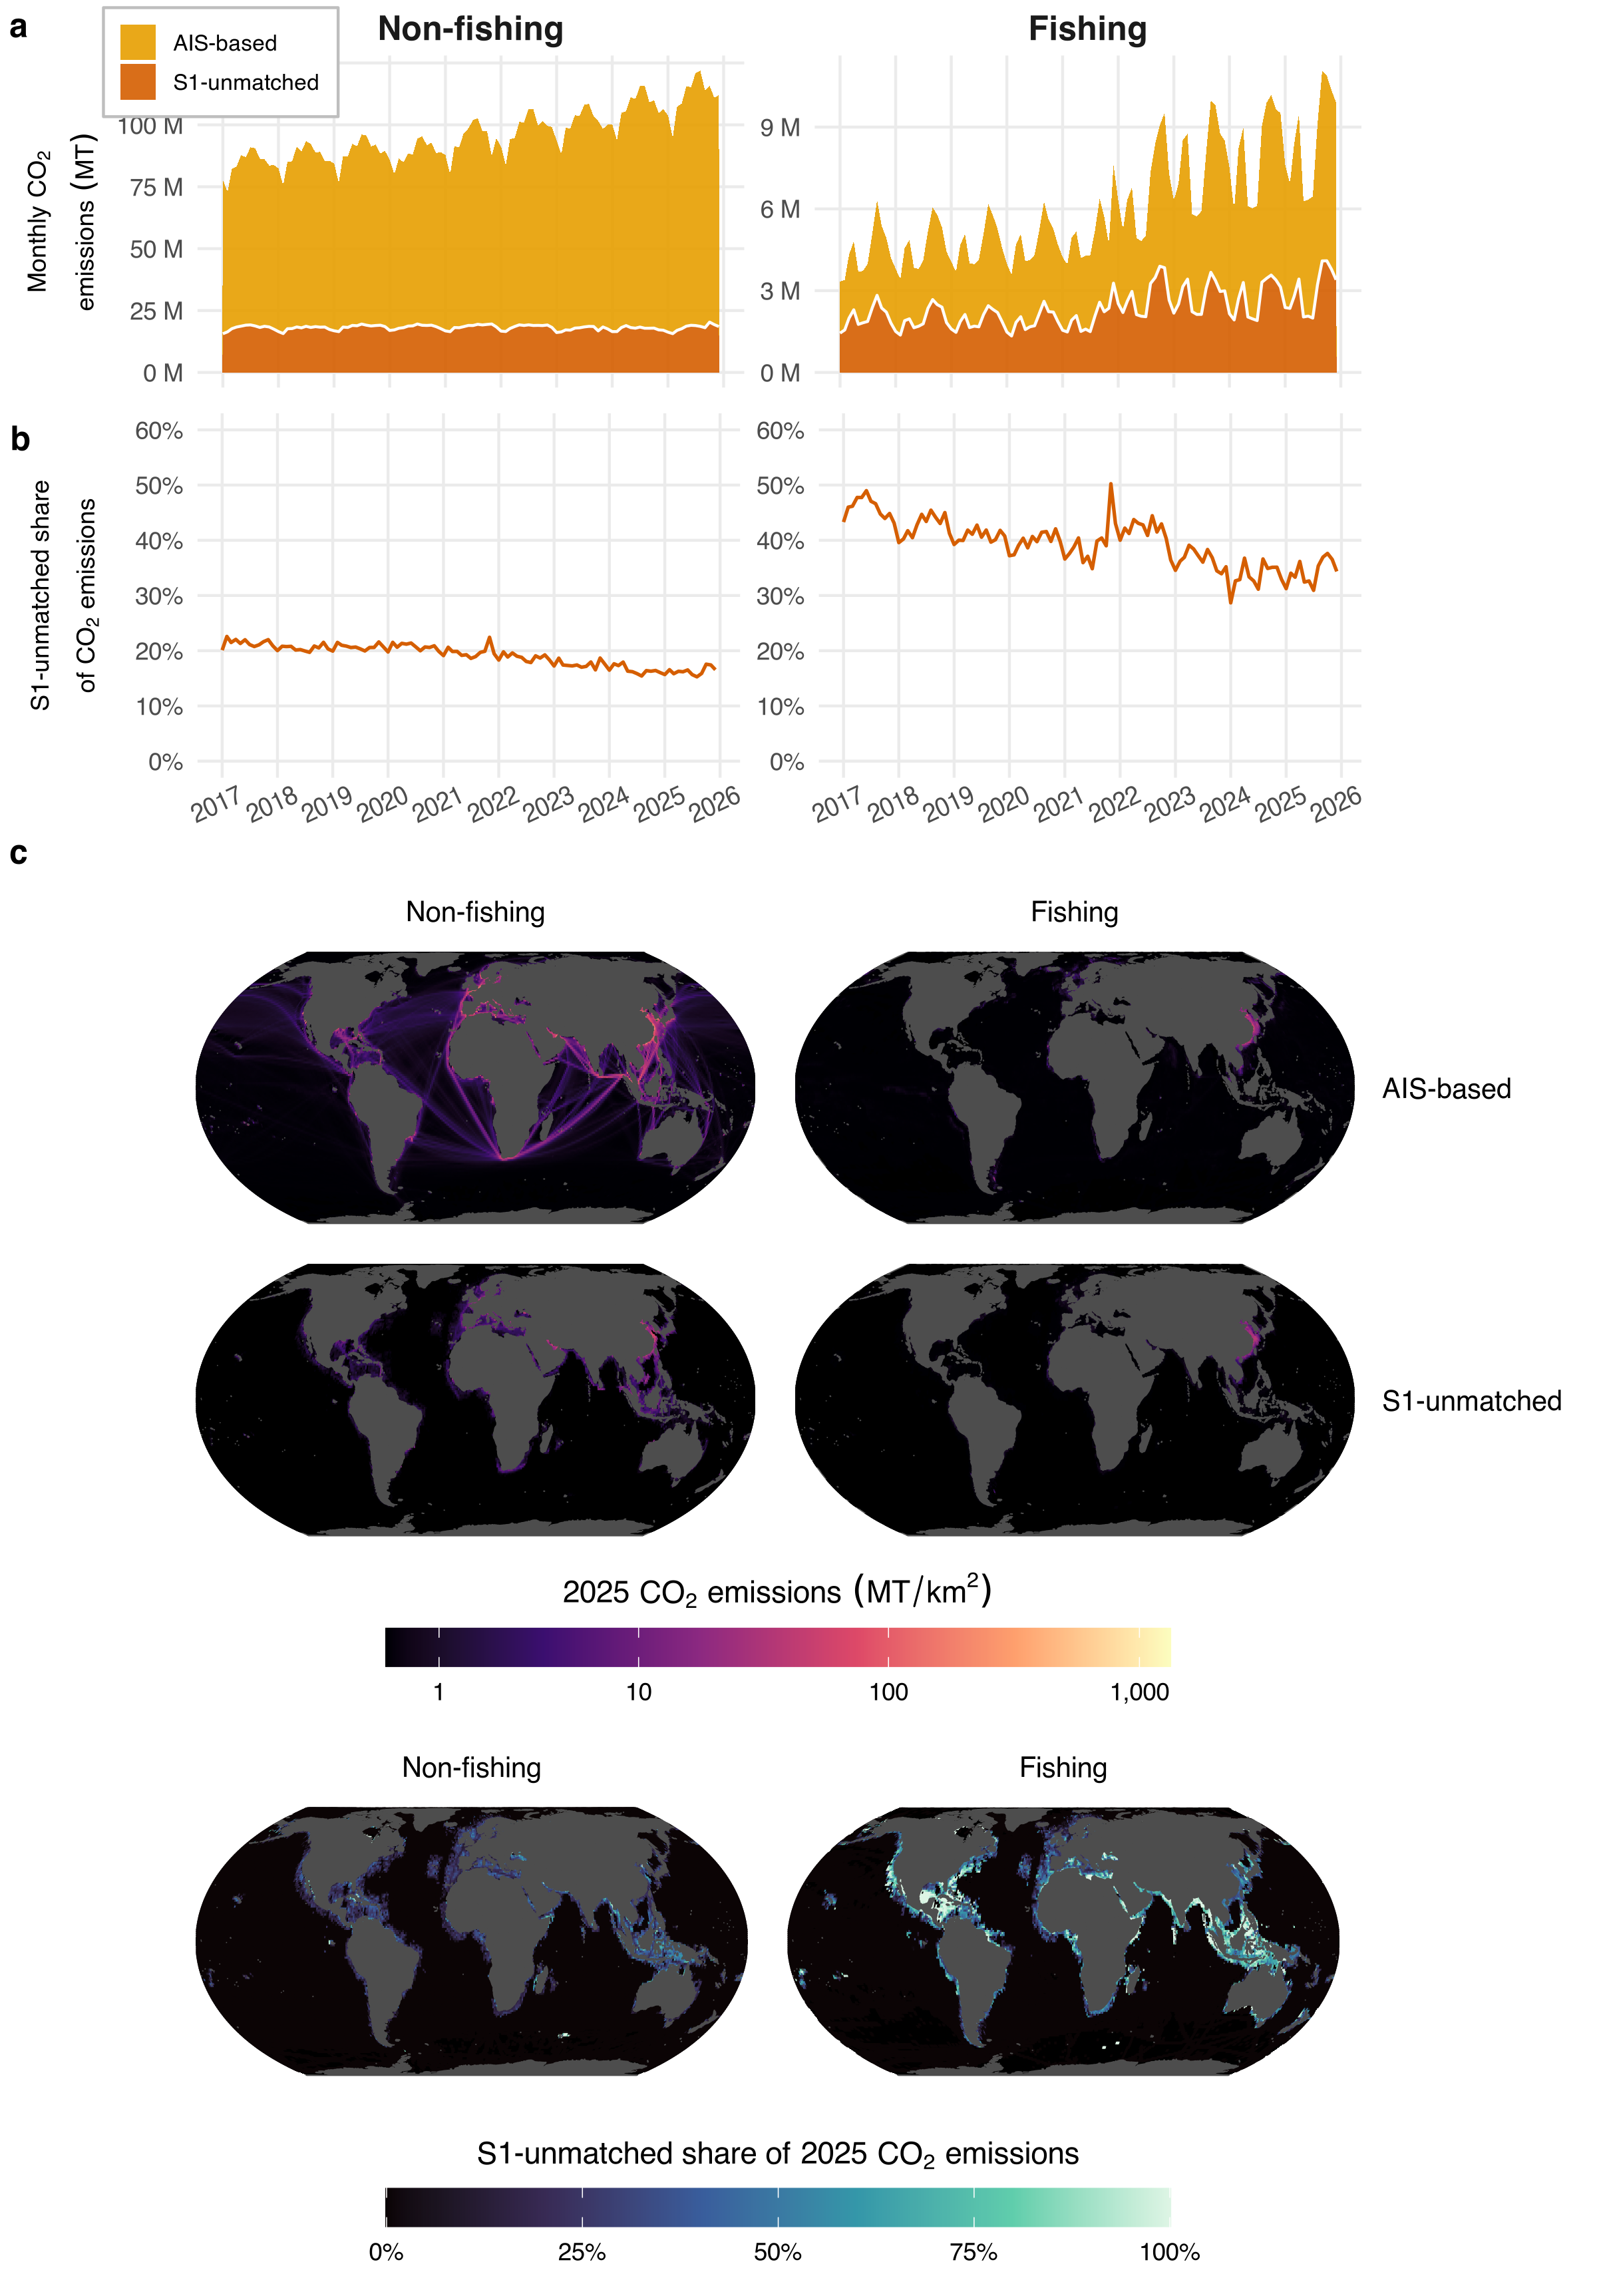
\includegraphics[width=\columnwidth]{figures/fig-spatial-temporal-richness-by-fleet-total-pseudolog-1.png}
    \caption{The fishing and non-fishing components of Figure \ref{fig:fig-emissions-time-series-and-maps}, panel for panel. (a) Time series of monthly global CO$_2$ emissions, shown for both AIS-based and S1-unmatched emissions, and for both fishing and non-fishing vessels. (b) Time series of the monthly share of global CO$_{2}$ emissions that is S1-unmatched, for both fishing and non-fishing vessels. (c) Spatial distribution of 2025 CO$_{2}$ emissions, AIS-based (top) and S1-unmatched (middle), for both fishing and non-fishing vessels (columns), shown at a 1x1 degree spatial resolution; emissions are area-normalized for each pixel (metric tonnes per square kilometer, shown on a pseudolog-10 scale). The bottom maps show, for each pixel, the share of its 2025 CO$_{2}$ emissions from that group of vessels that is S1-unmatched; unlike the maps above them, these show a percentage and use their own color scale. Pixels with no 2025 emissions from the group are drawn in the background color, as are pixels with no emissions on the maps above.}
    \label{fig:fig-spatial-temporal-richness-by-fleet-total-pseudolog}
\end{figure}

\begin{figure}[H]
    \centering
    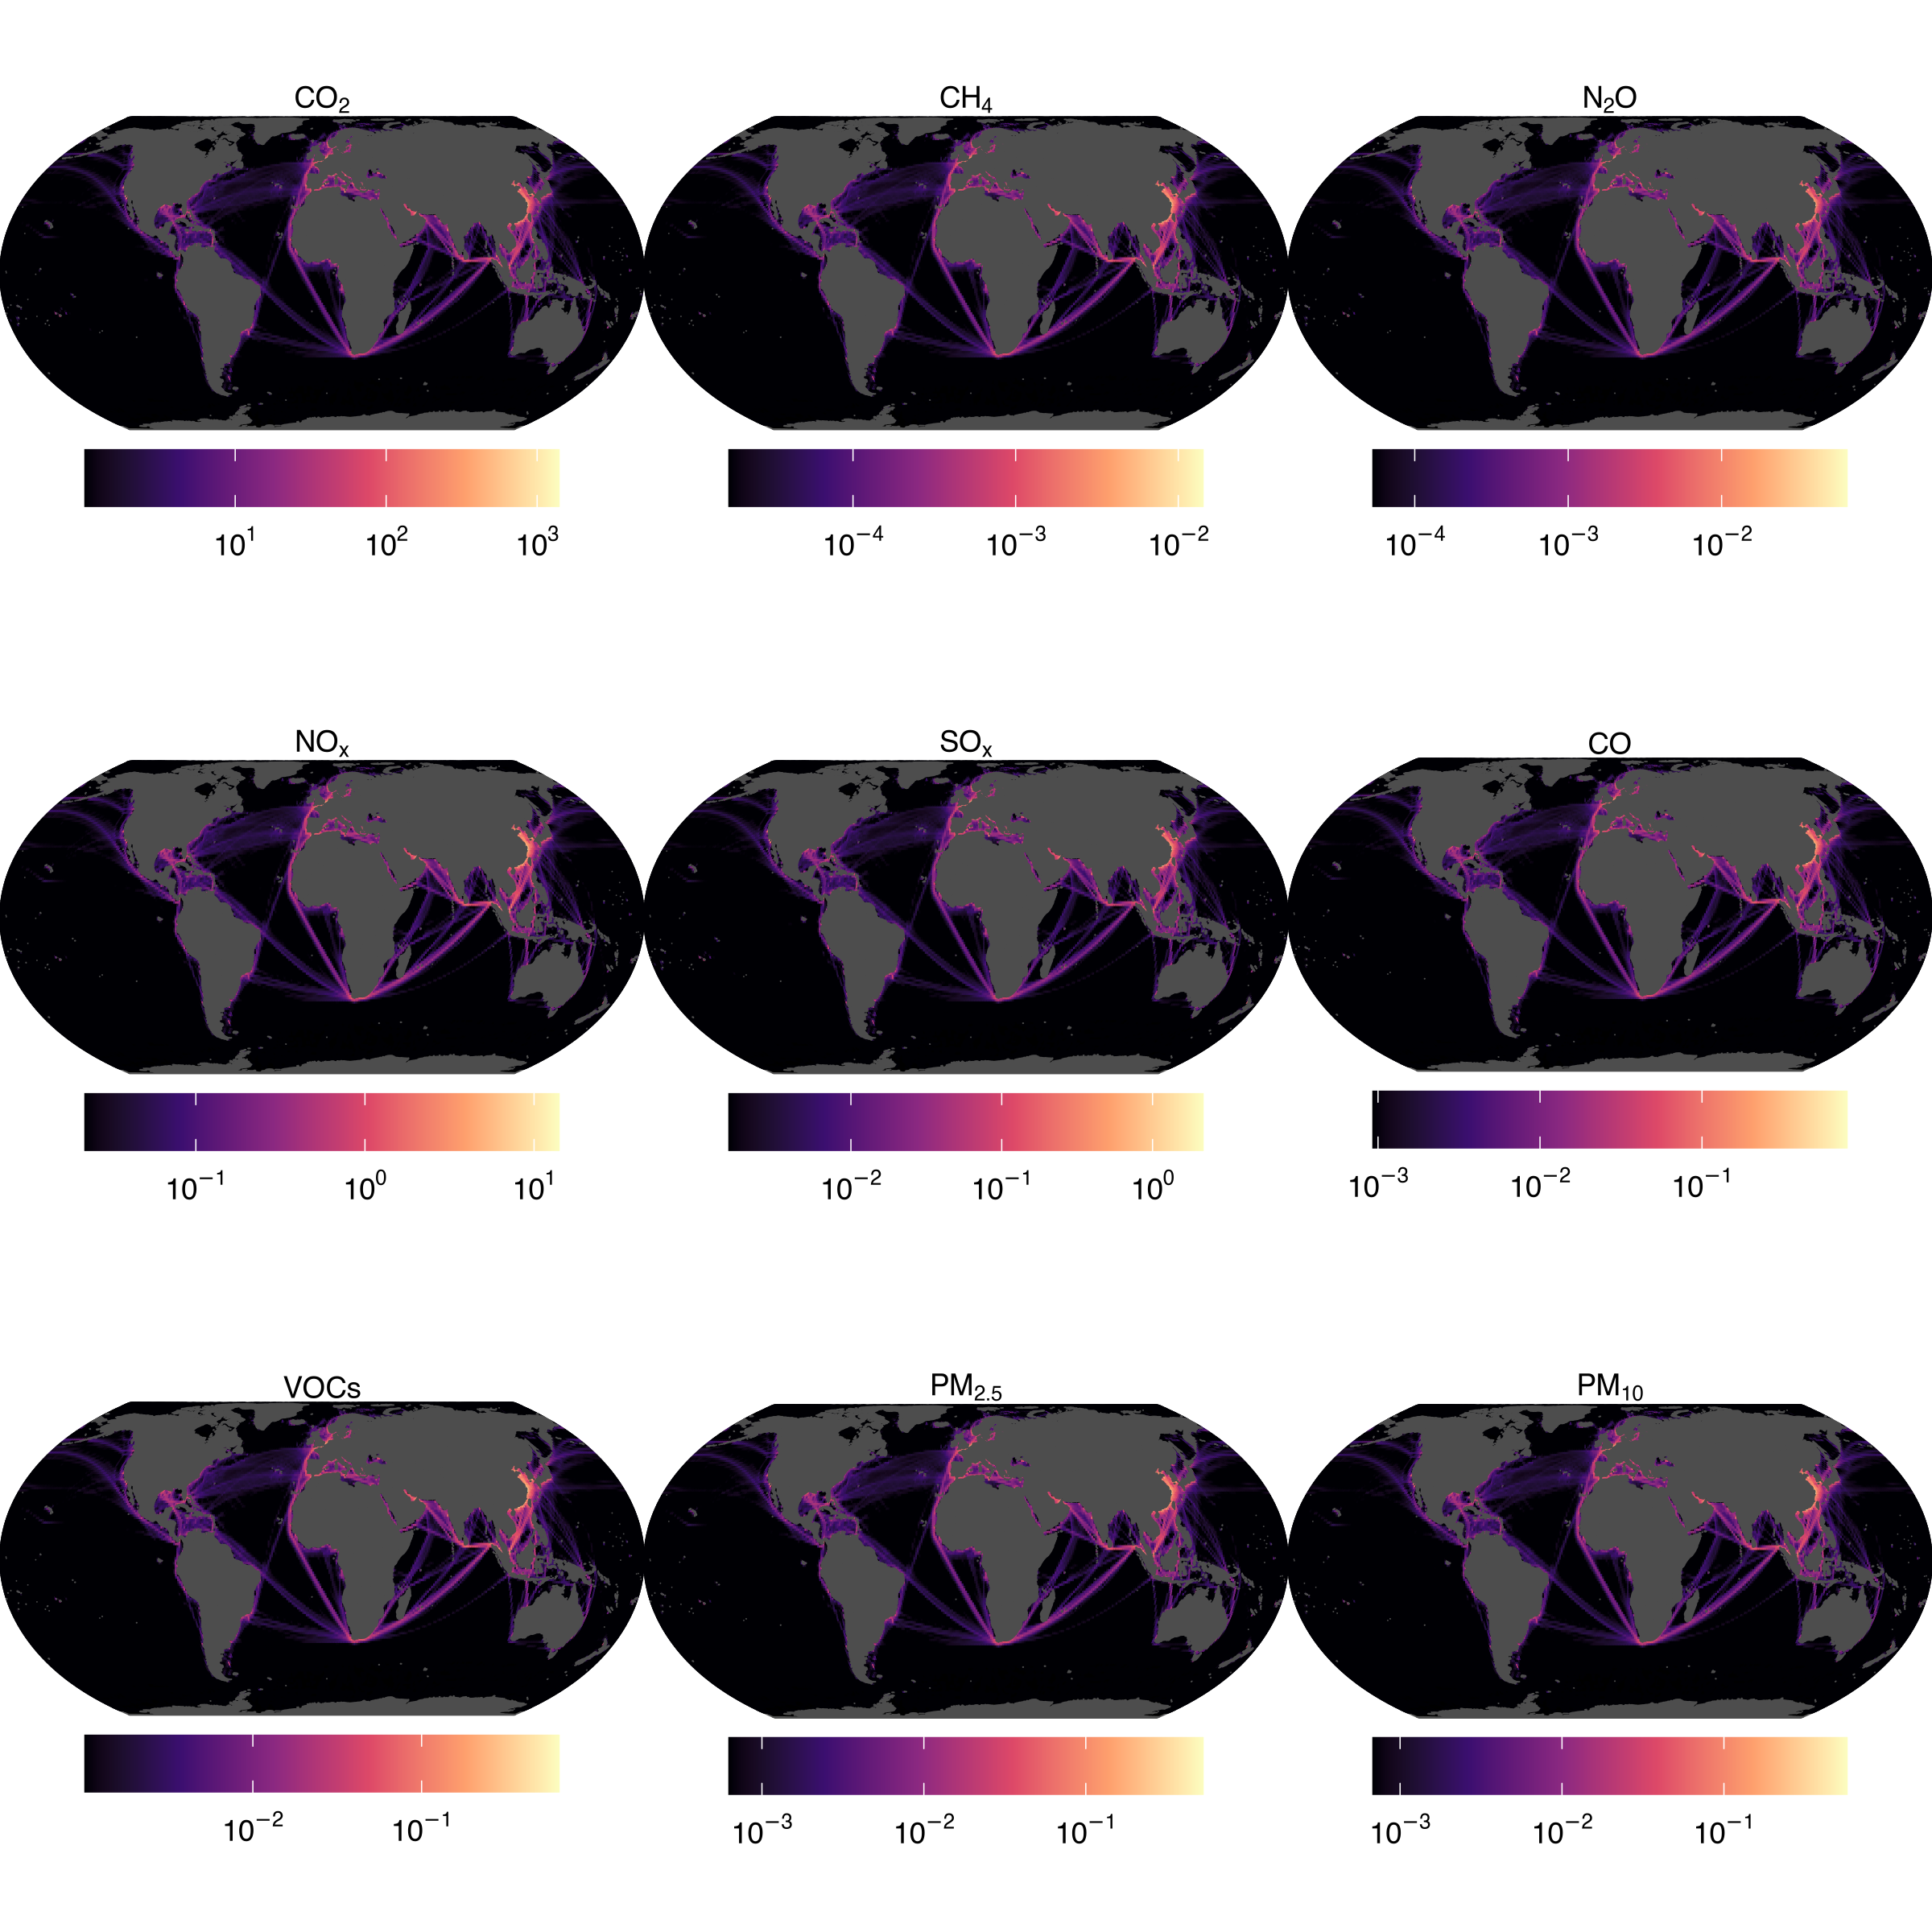
\includegraphics[width=\columnwidth]{figures/fig-pollutant-maps-qlog10-1.png}
    \caption{Spatial maps of 2025 emissions for each GHG and pollutant, aggregated across AIS-based and S1-unmatched emissions, and shown at a 1x1 degree spatial resolution. Emissions are area-normalized for each pixel (metric tonnes per square kilometer) and shown using a log-10 scale. Each panel is scaled independently, spanning the 75th percentile to the maximum of that pollutant, with lower values drawn in the darkest color; colors are therefore not comparable between panels.}
    \label{fig:fig-pollutant-maps}
\end{figure}

\begin{figure}[H]
    \centering
    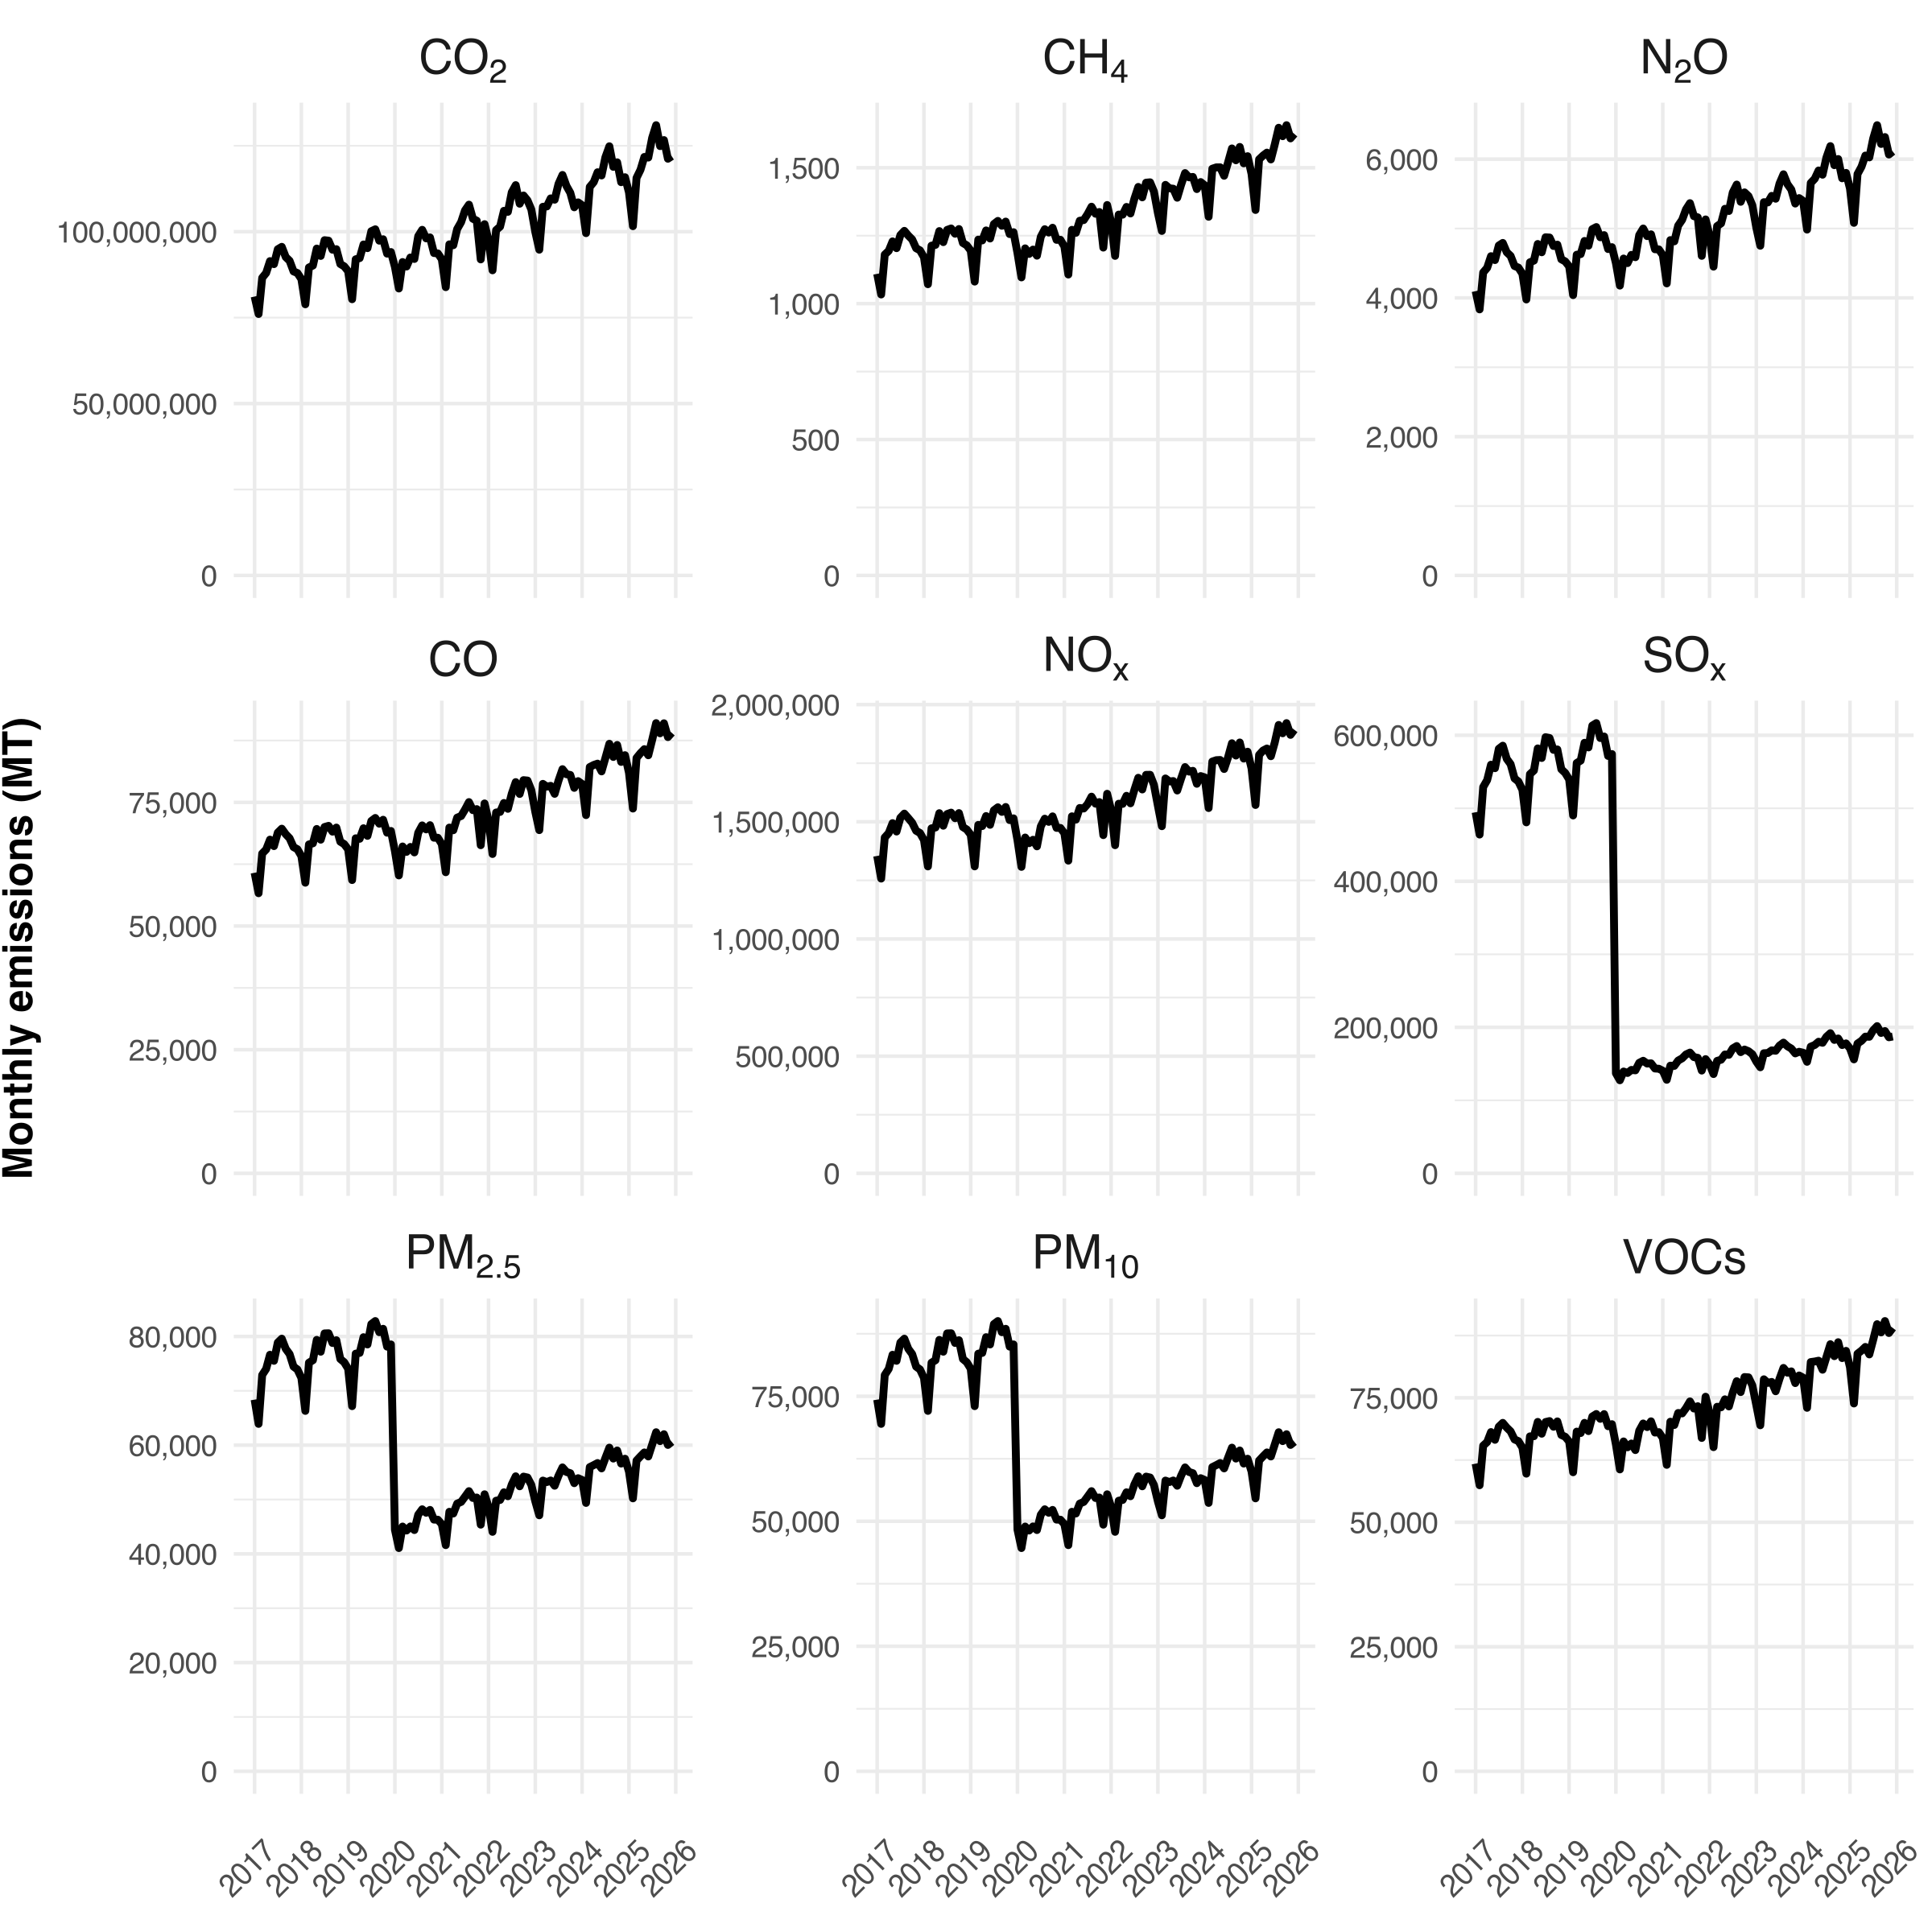
\includegraphics[width=\columnwidth]{figures/fig-pollutant-time-series-1.png}
    \caption{Time series of monthly global emissions for each GHG and pollutant, aggregated across AIS-based and S1-unmatched emissions.}
    \label{fig:fig-pollutant-time-series}
\end{figure}

\begin{figure}[H]
    \centering
    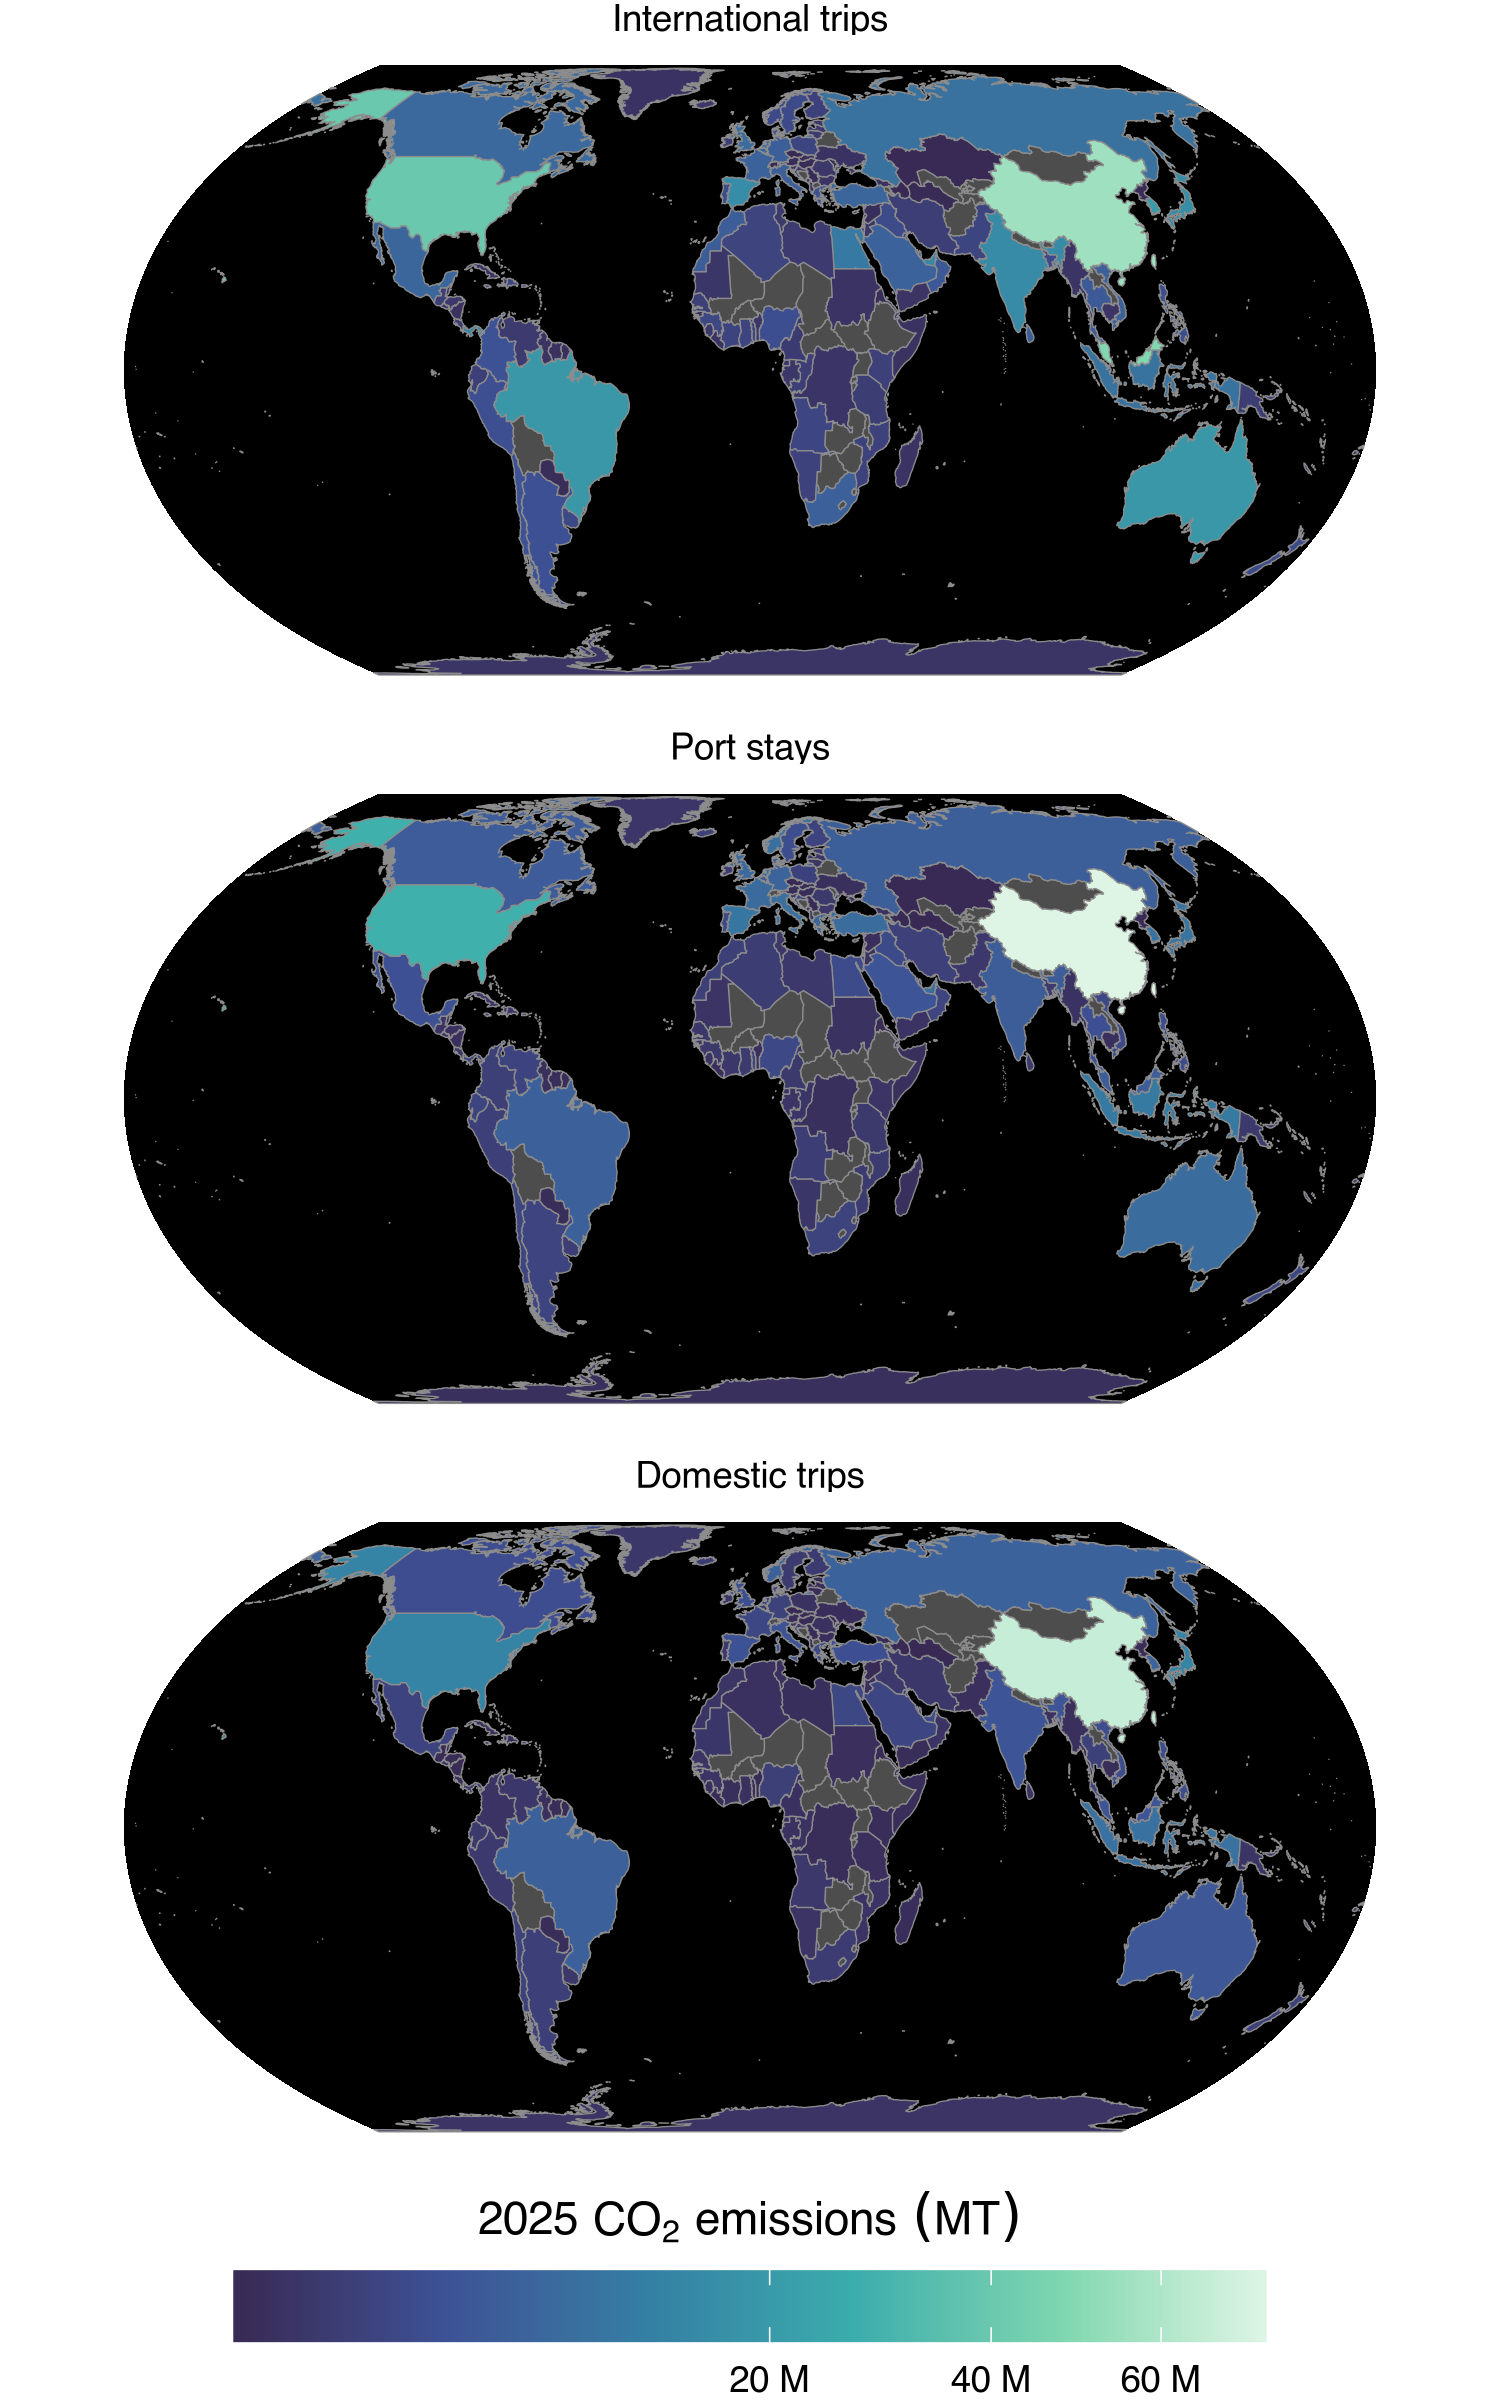
\includegraphics[width=0.85\columnwidth]{figures/fig-emissions-by-country-and-activity-type-1.png}
    \caption{CO$_{2}$ emissions by country for AIS-broadcasting vessels during different activity types (international trips, port stays, and domestic trips), aggregated for activities ending in 2025. Emissions for each international trip are partitioned equally to its departure and arrival country. The color scale is square-root transformed, so that lower-emitting countries remain distinguishable alongside the largest emitters. Countries with no values are shown in gray.}
    \label{fig:fig-emissions-by-country-and-activity-type}
\end{figure}

\begin{figure}[H]
    \centering
    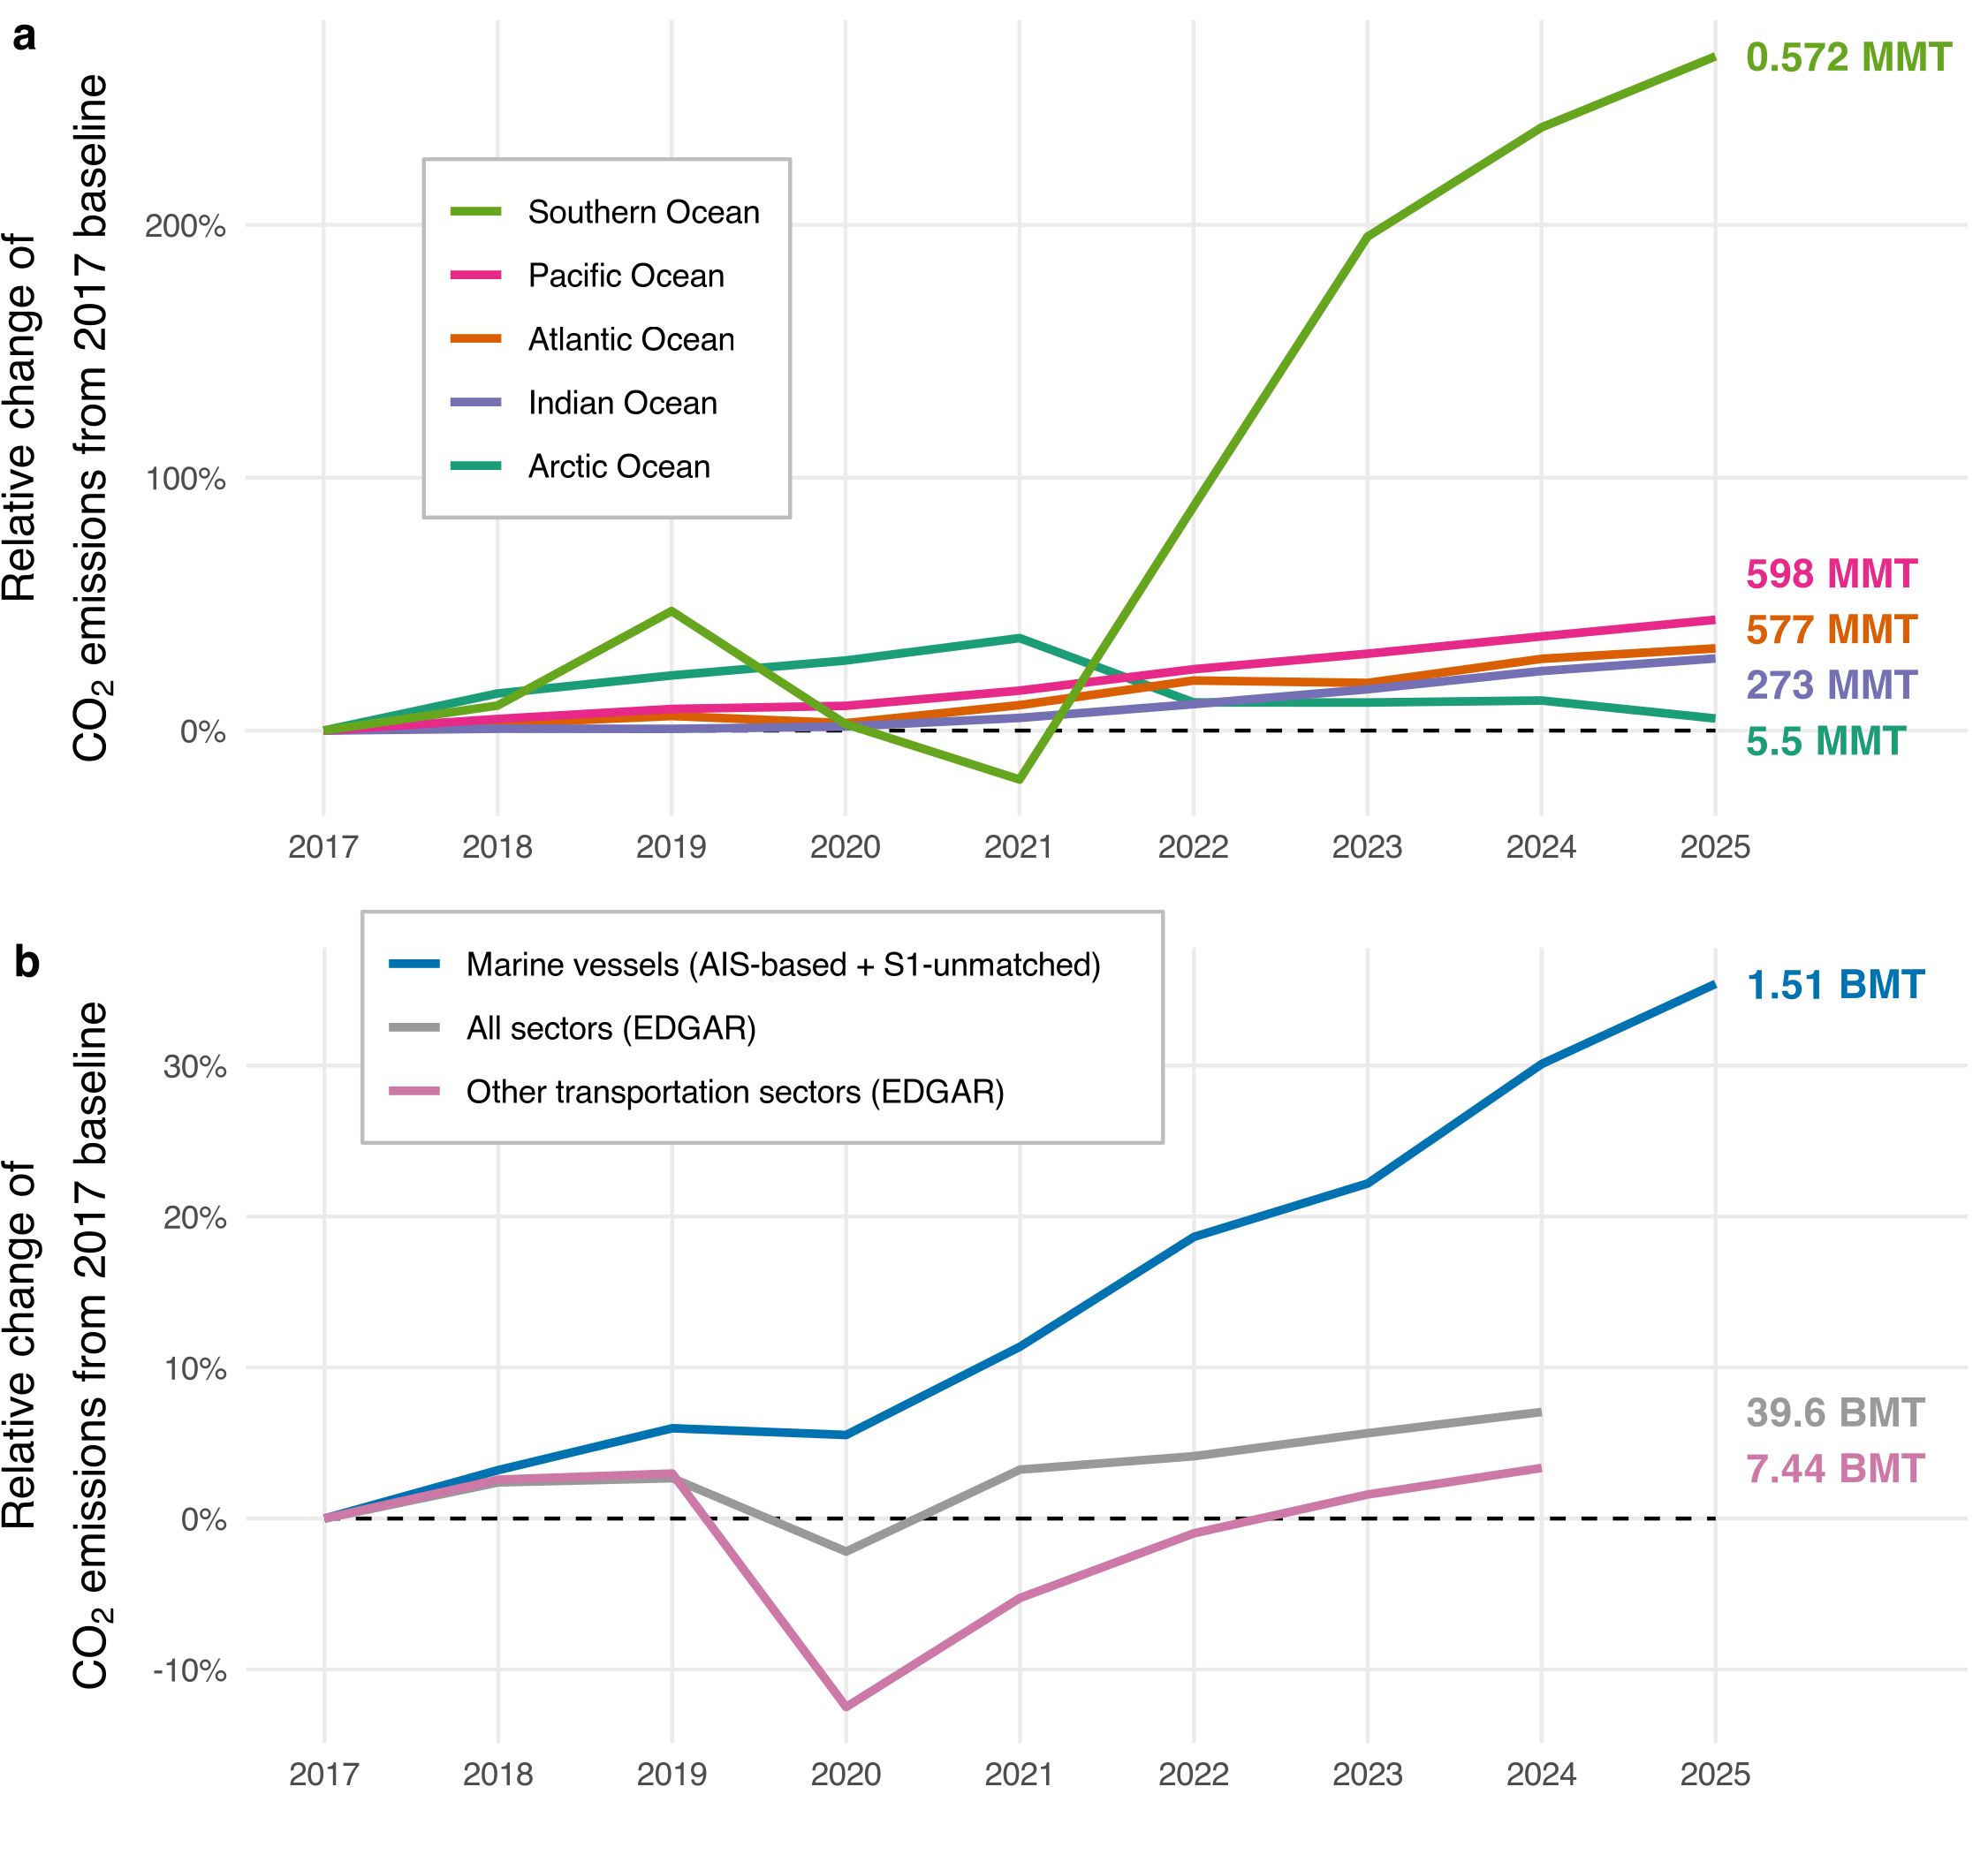
\includegraphics[width=\columnwidth]{figures/fig-emissions-marine-ocean-other-1.png}
    \caption{Trend in CO$_{2}$ emissions by ocean (normalized to 2017 baseline), using our fused (AIS-based + S1-unmatched) estimates. On the right-hand side of the figure, absolute values for the last year of available data (2025) are shown as text and color-coded for each line.}
    \label{fig:fig-emissions-marine-ocean-other}
\end{figure}

\begin{figure}[H]
    \centering
    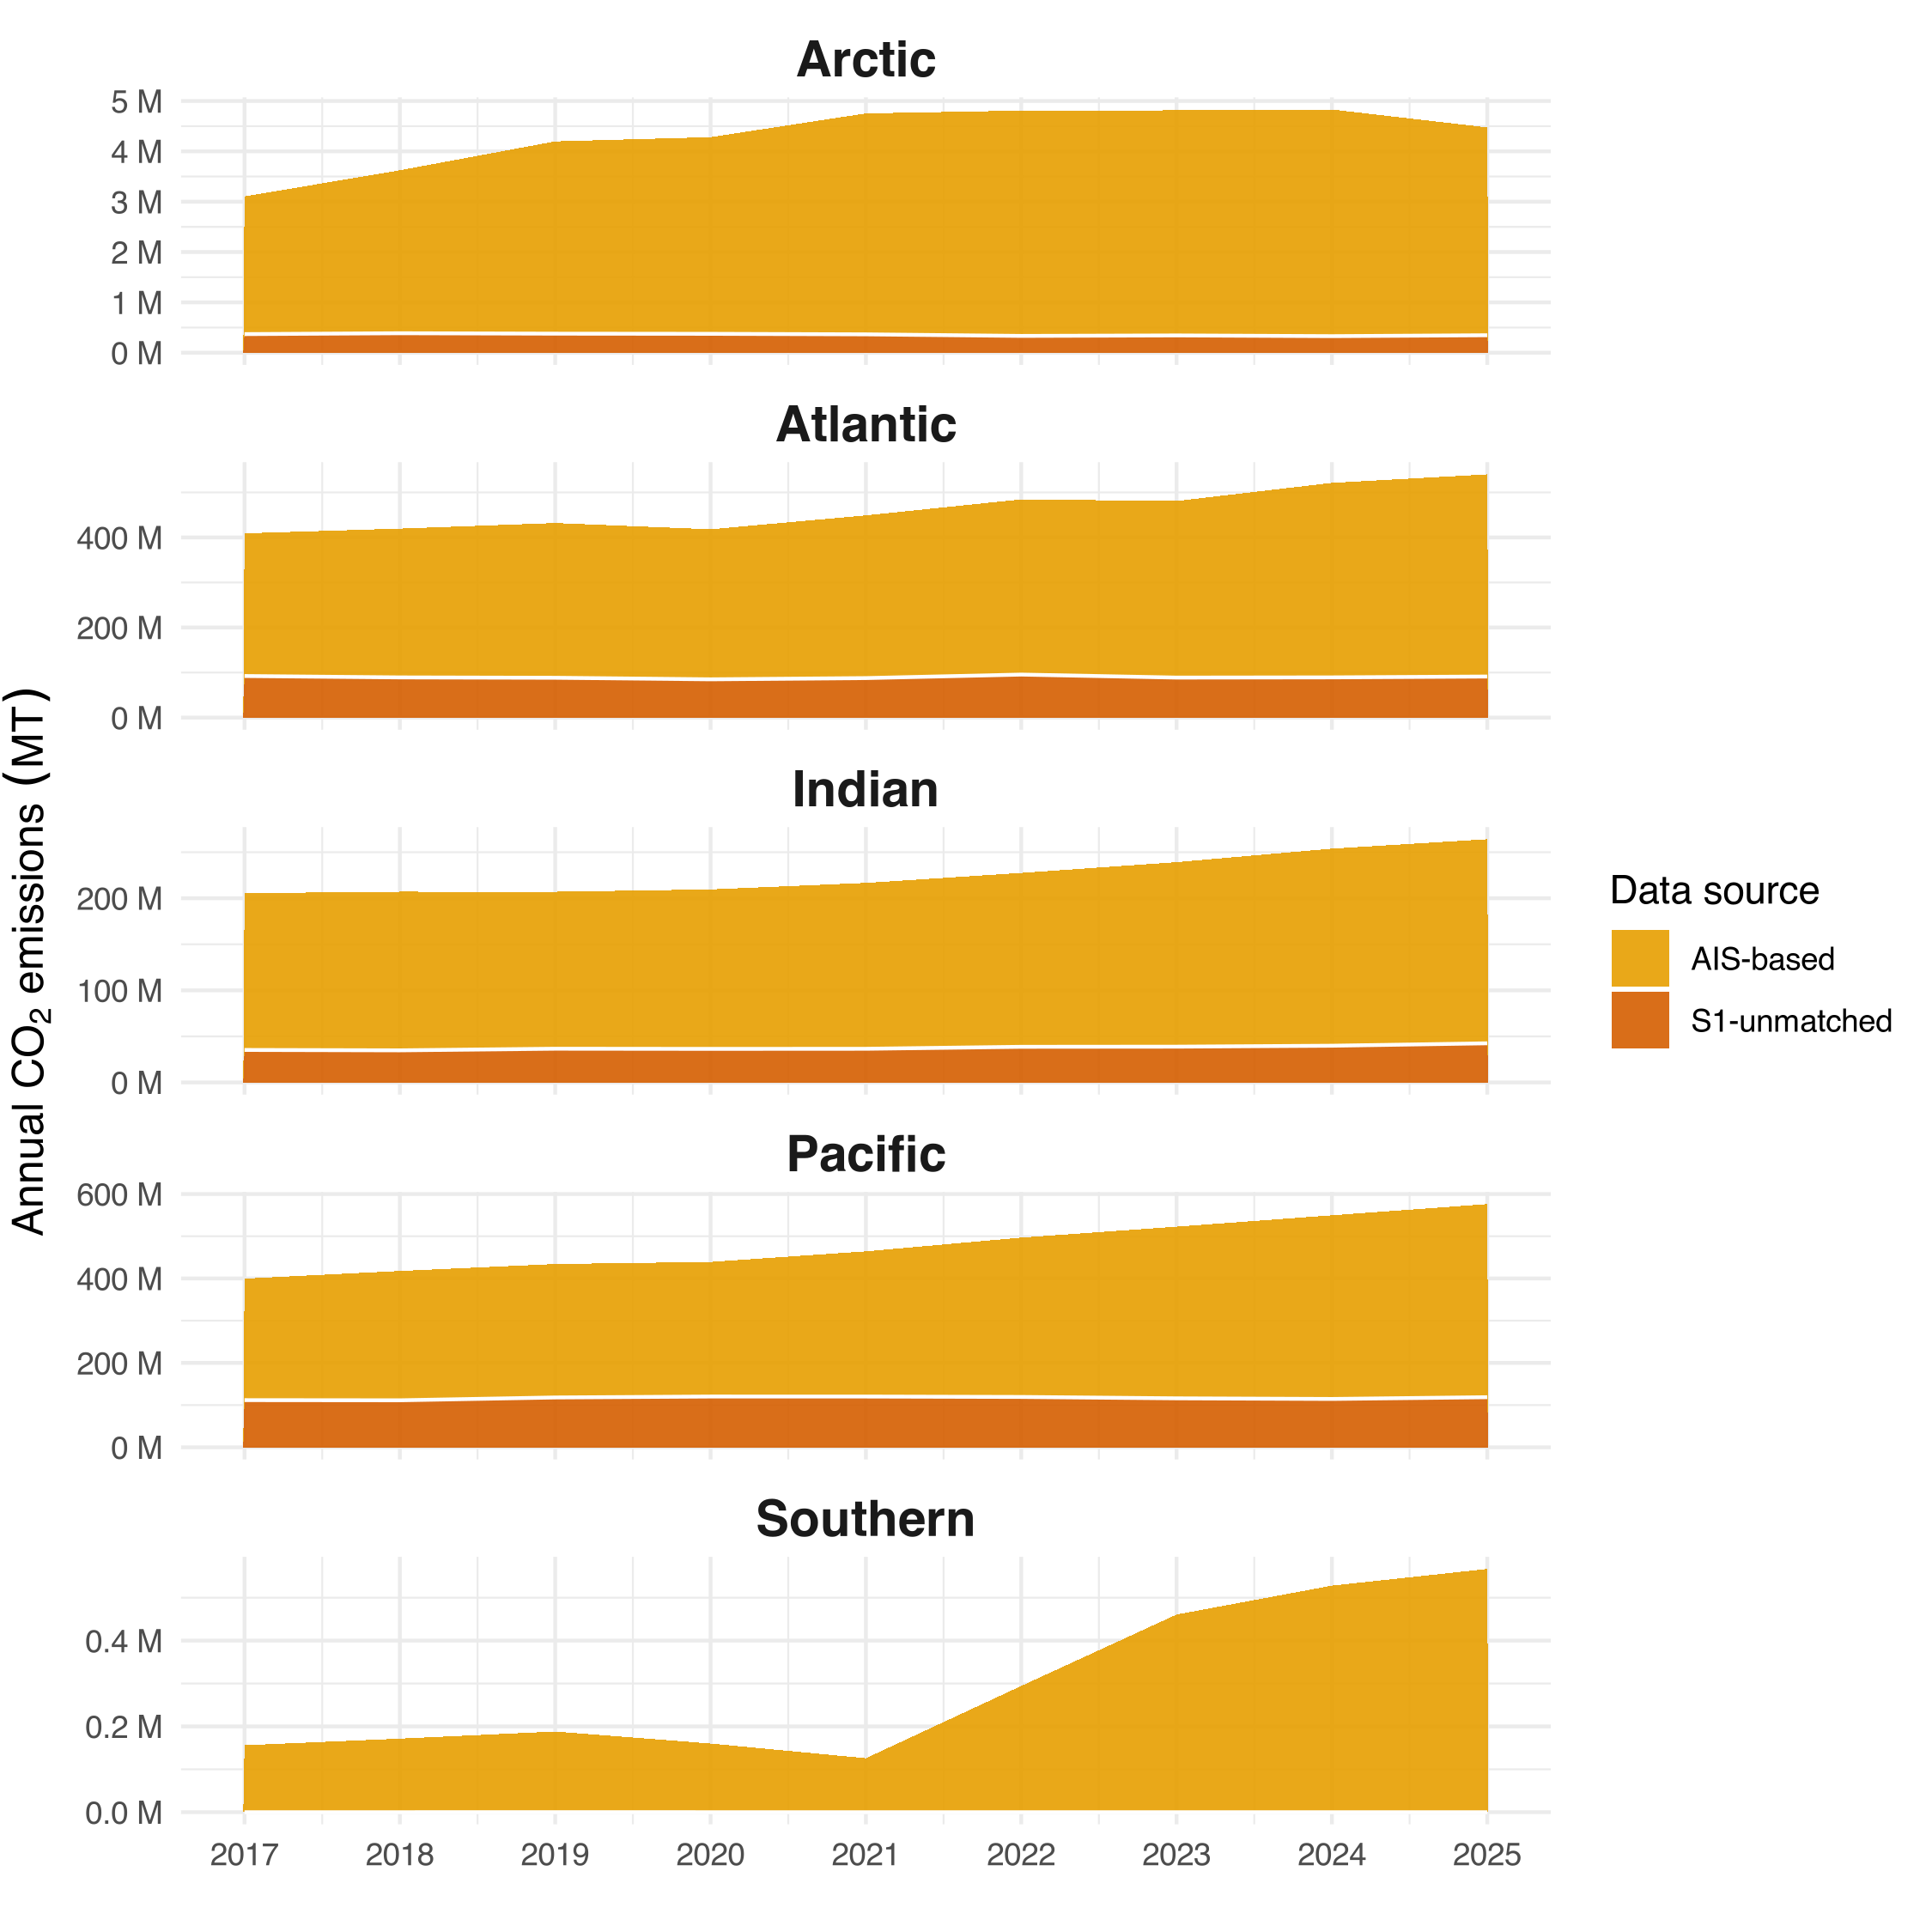
\includegraphics[width=\columnwidth]{figures/fig-annual-emissions-by-ocean-and-data-source-1.png}
    \caption{Annual total CO$_{2}$ emissions by ocean, disaggregated by data source (AIS-based and S1-unmatched).}
    \label{fig:fig-annual-emissions-by-ocean-and-data-source}
\end{figure}

\begin{figure}[!p]
    \centering
    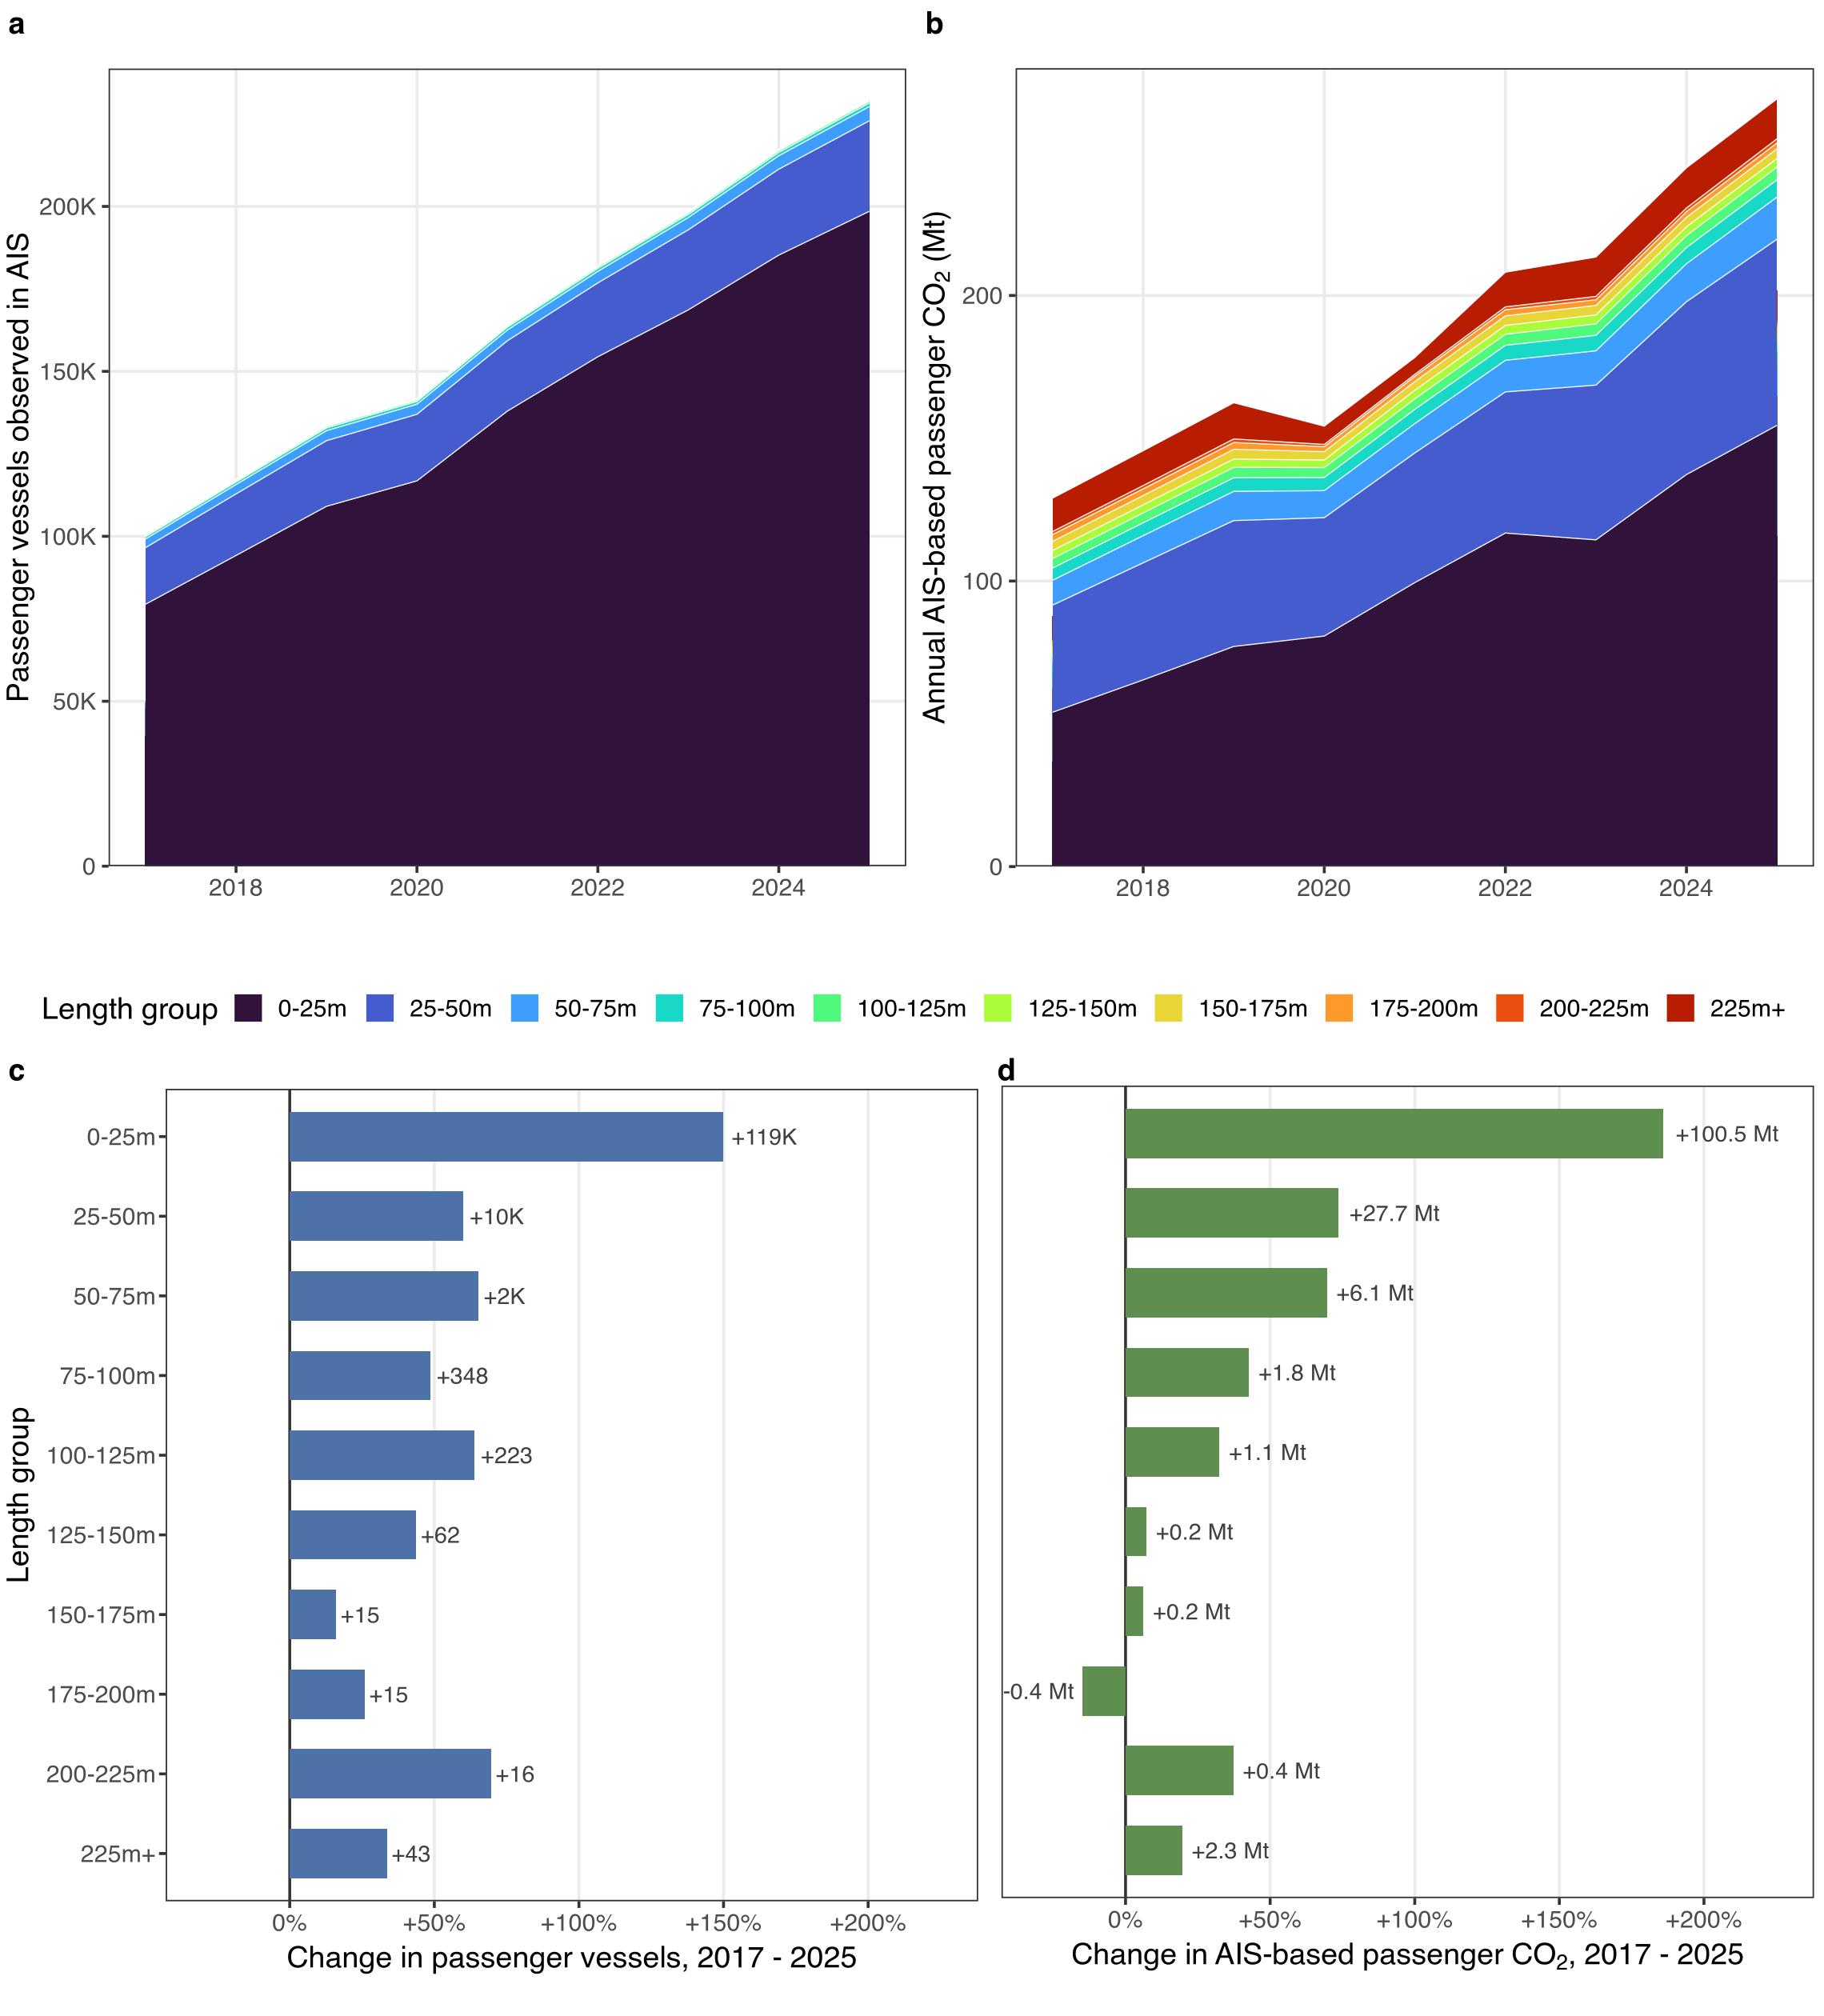
\includegraphics[width=\columnwidth,height=0.92\textheight,keepaspectratio]{figures/figS-passenger-size-panels-1.png}
    \caption{Passenger vessels by length bin, 2017 against 2025, showing growth concentrated in the smallest sizes.}
    \label{fig:figS-passenger-size-panels}
\end{figure}

\begin{figure}[H]
    \centering
    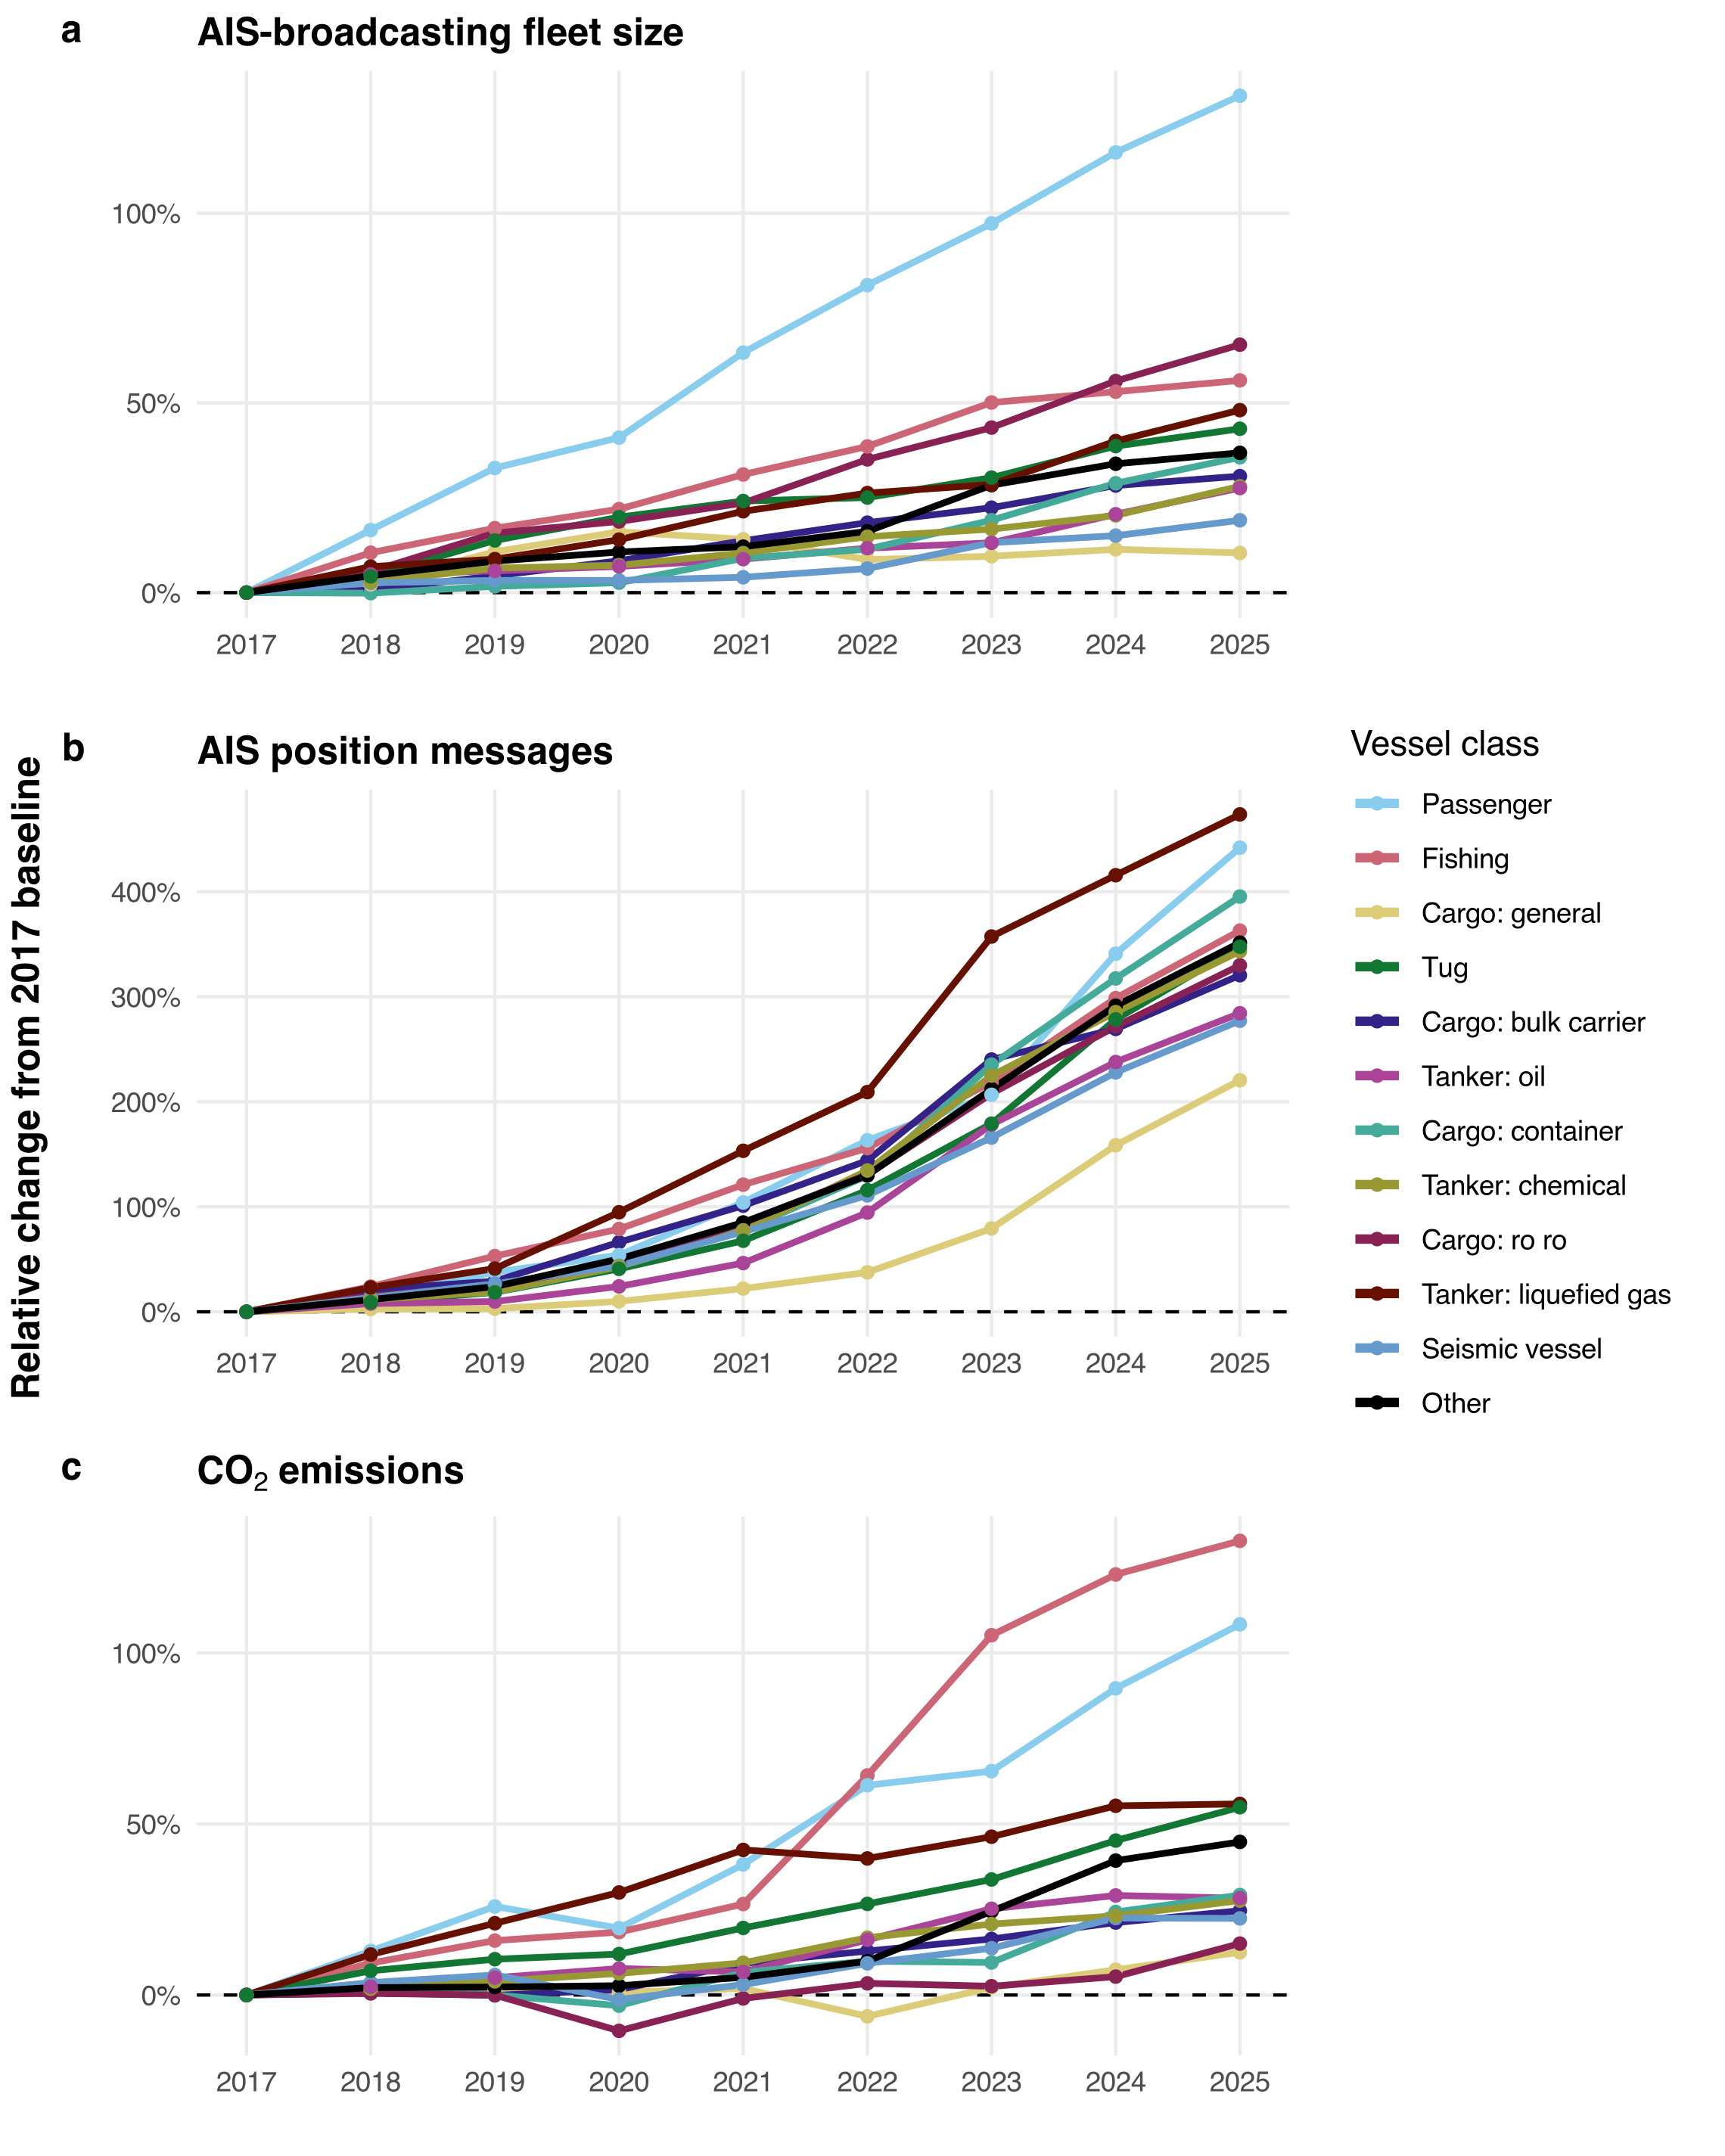
\includegraphics[width=\columnwidth]{figures/figS-fleet-growth-by-year-1.png}
    \caption{Relative change since 2017, by vessel class, in (a) the number of AIS-broadcasting vessels, (b) AIS position messages received, and (c) CO$_{2}$ emissions, for AIS-broadcasting vessels. Every panel is expressed as a change from that class's own 2017 value, so classes of very different absolute size can be read on a single scale. Growth in panels a and b reflects both real expansion of the fleet and its activity, and the increasing uptake and reception of AIS over the period. Passenger vessels grow fastest in fleet size and fishing vessels fastest in emissions, the two classes that other inventories are least likely to cover.}
    \label{fig:figS-fleet-growth-by-year}
\end{figure}

\begin{figure}[H]
    \centering
    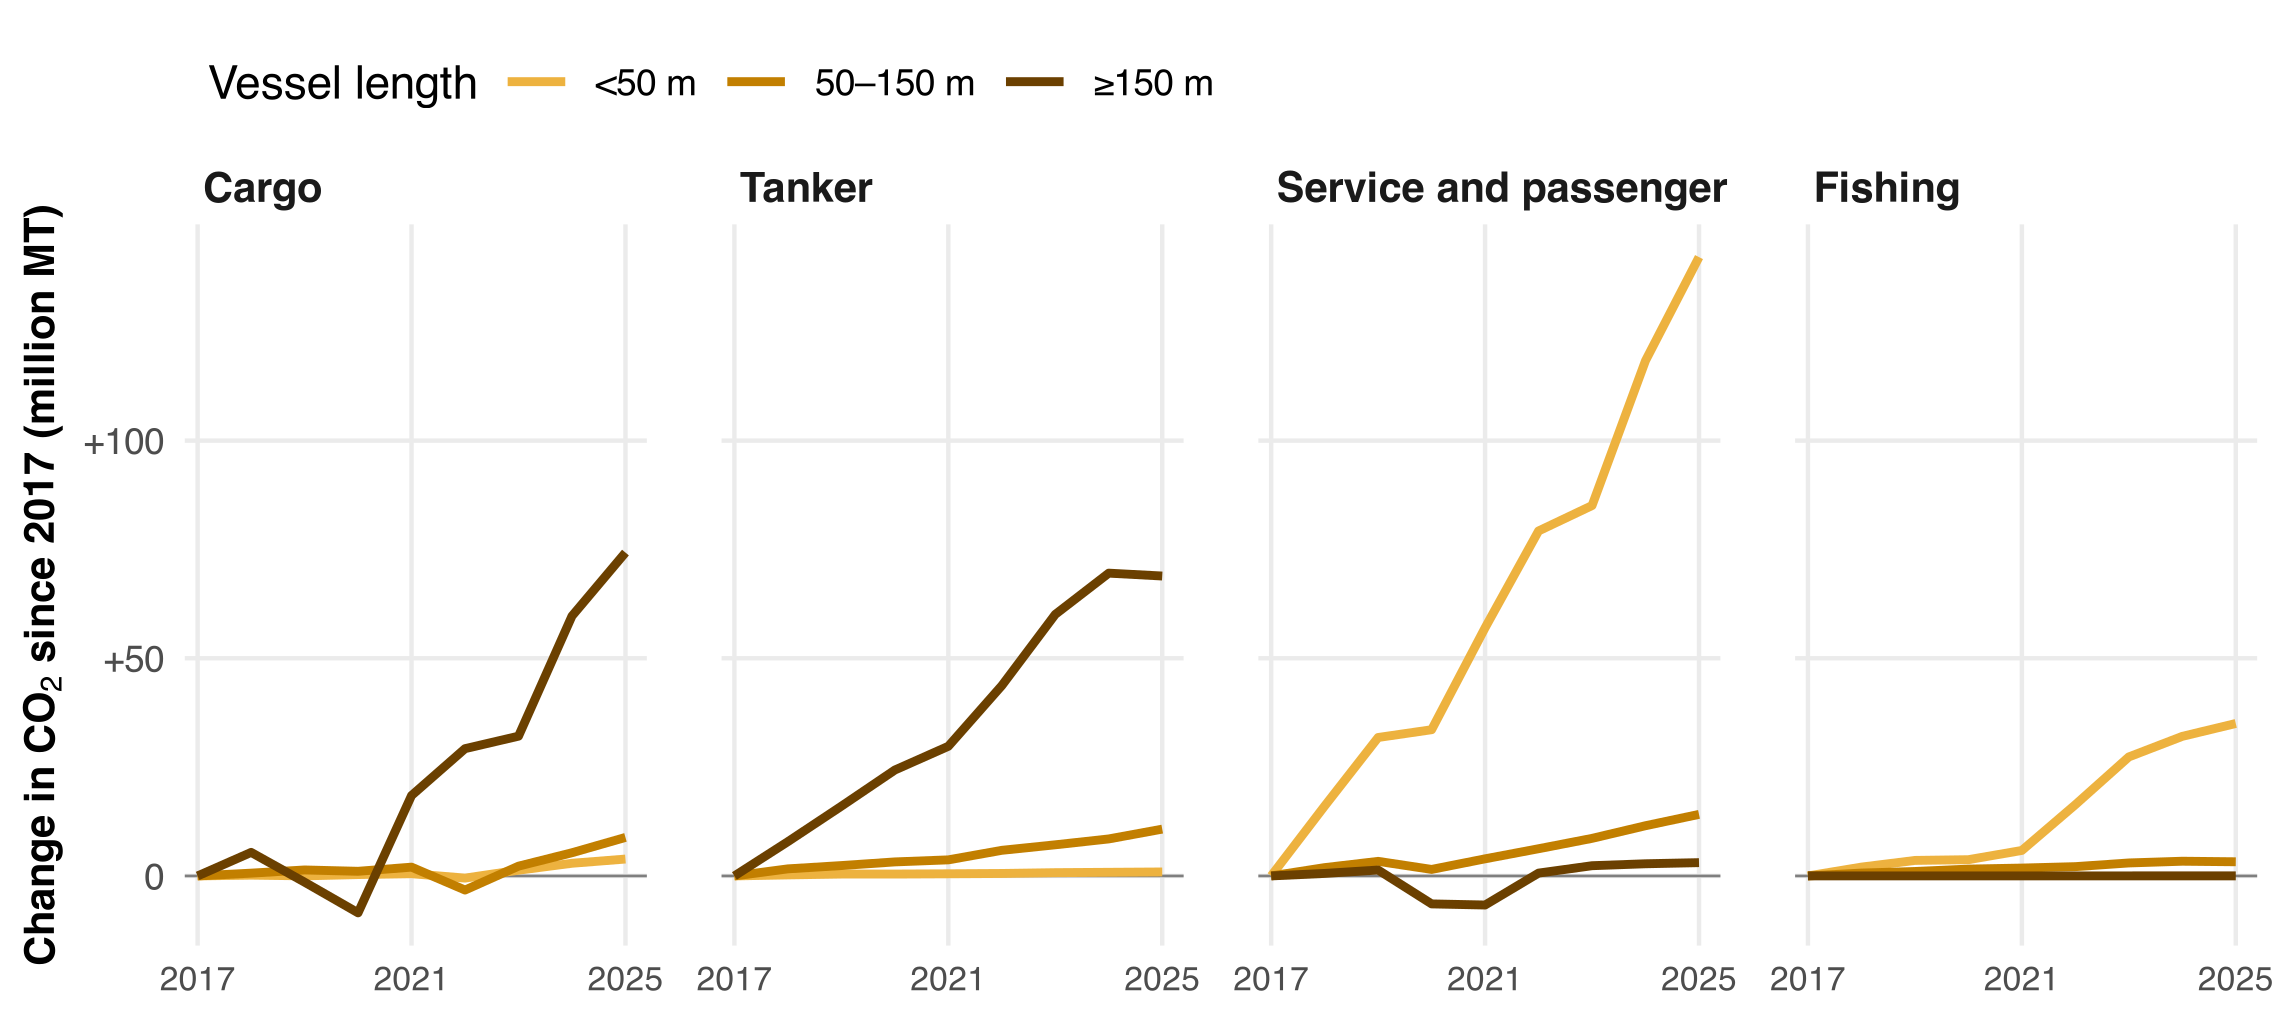
\includegraphics[width=\columnwidth]{figures/figS-growth-timeline-by-family-length-1.png}
    \caption{Change in AIS-based CO$_{2}$ emissions since 2017, by vessel class family and length band. Each line is a segment's annual emissions minus its 2017 emissions. Families are as in Fig. \ref{fig:fig-ais-data-richness} and length bands as in Supplementary Tables \ref{tab:growth_share_by_family_length} and \ref{tab:growth_decomposition_by_family_length}, so each line ends at that segment's emissions change in Supplementary Table \ref{tab:growth_decomposition_by_family_length}.}
    \label{fig:figS-growth-timeline-by-family-length}
\end{figure}

\begin{figure}[H]
    \centering
    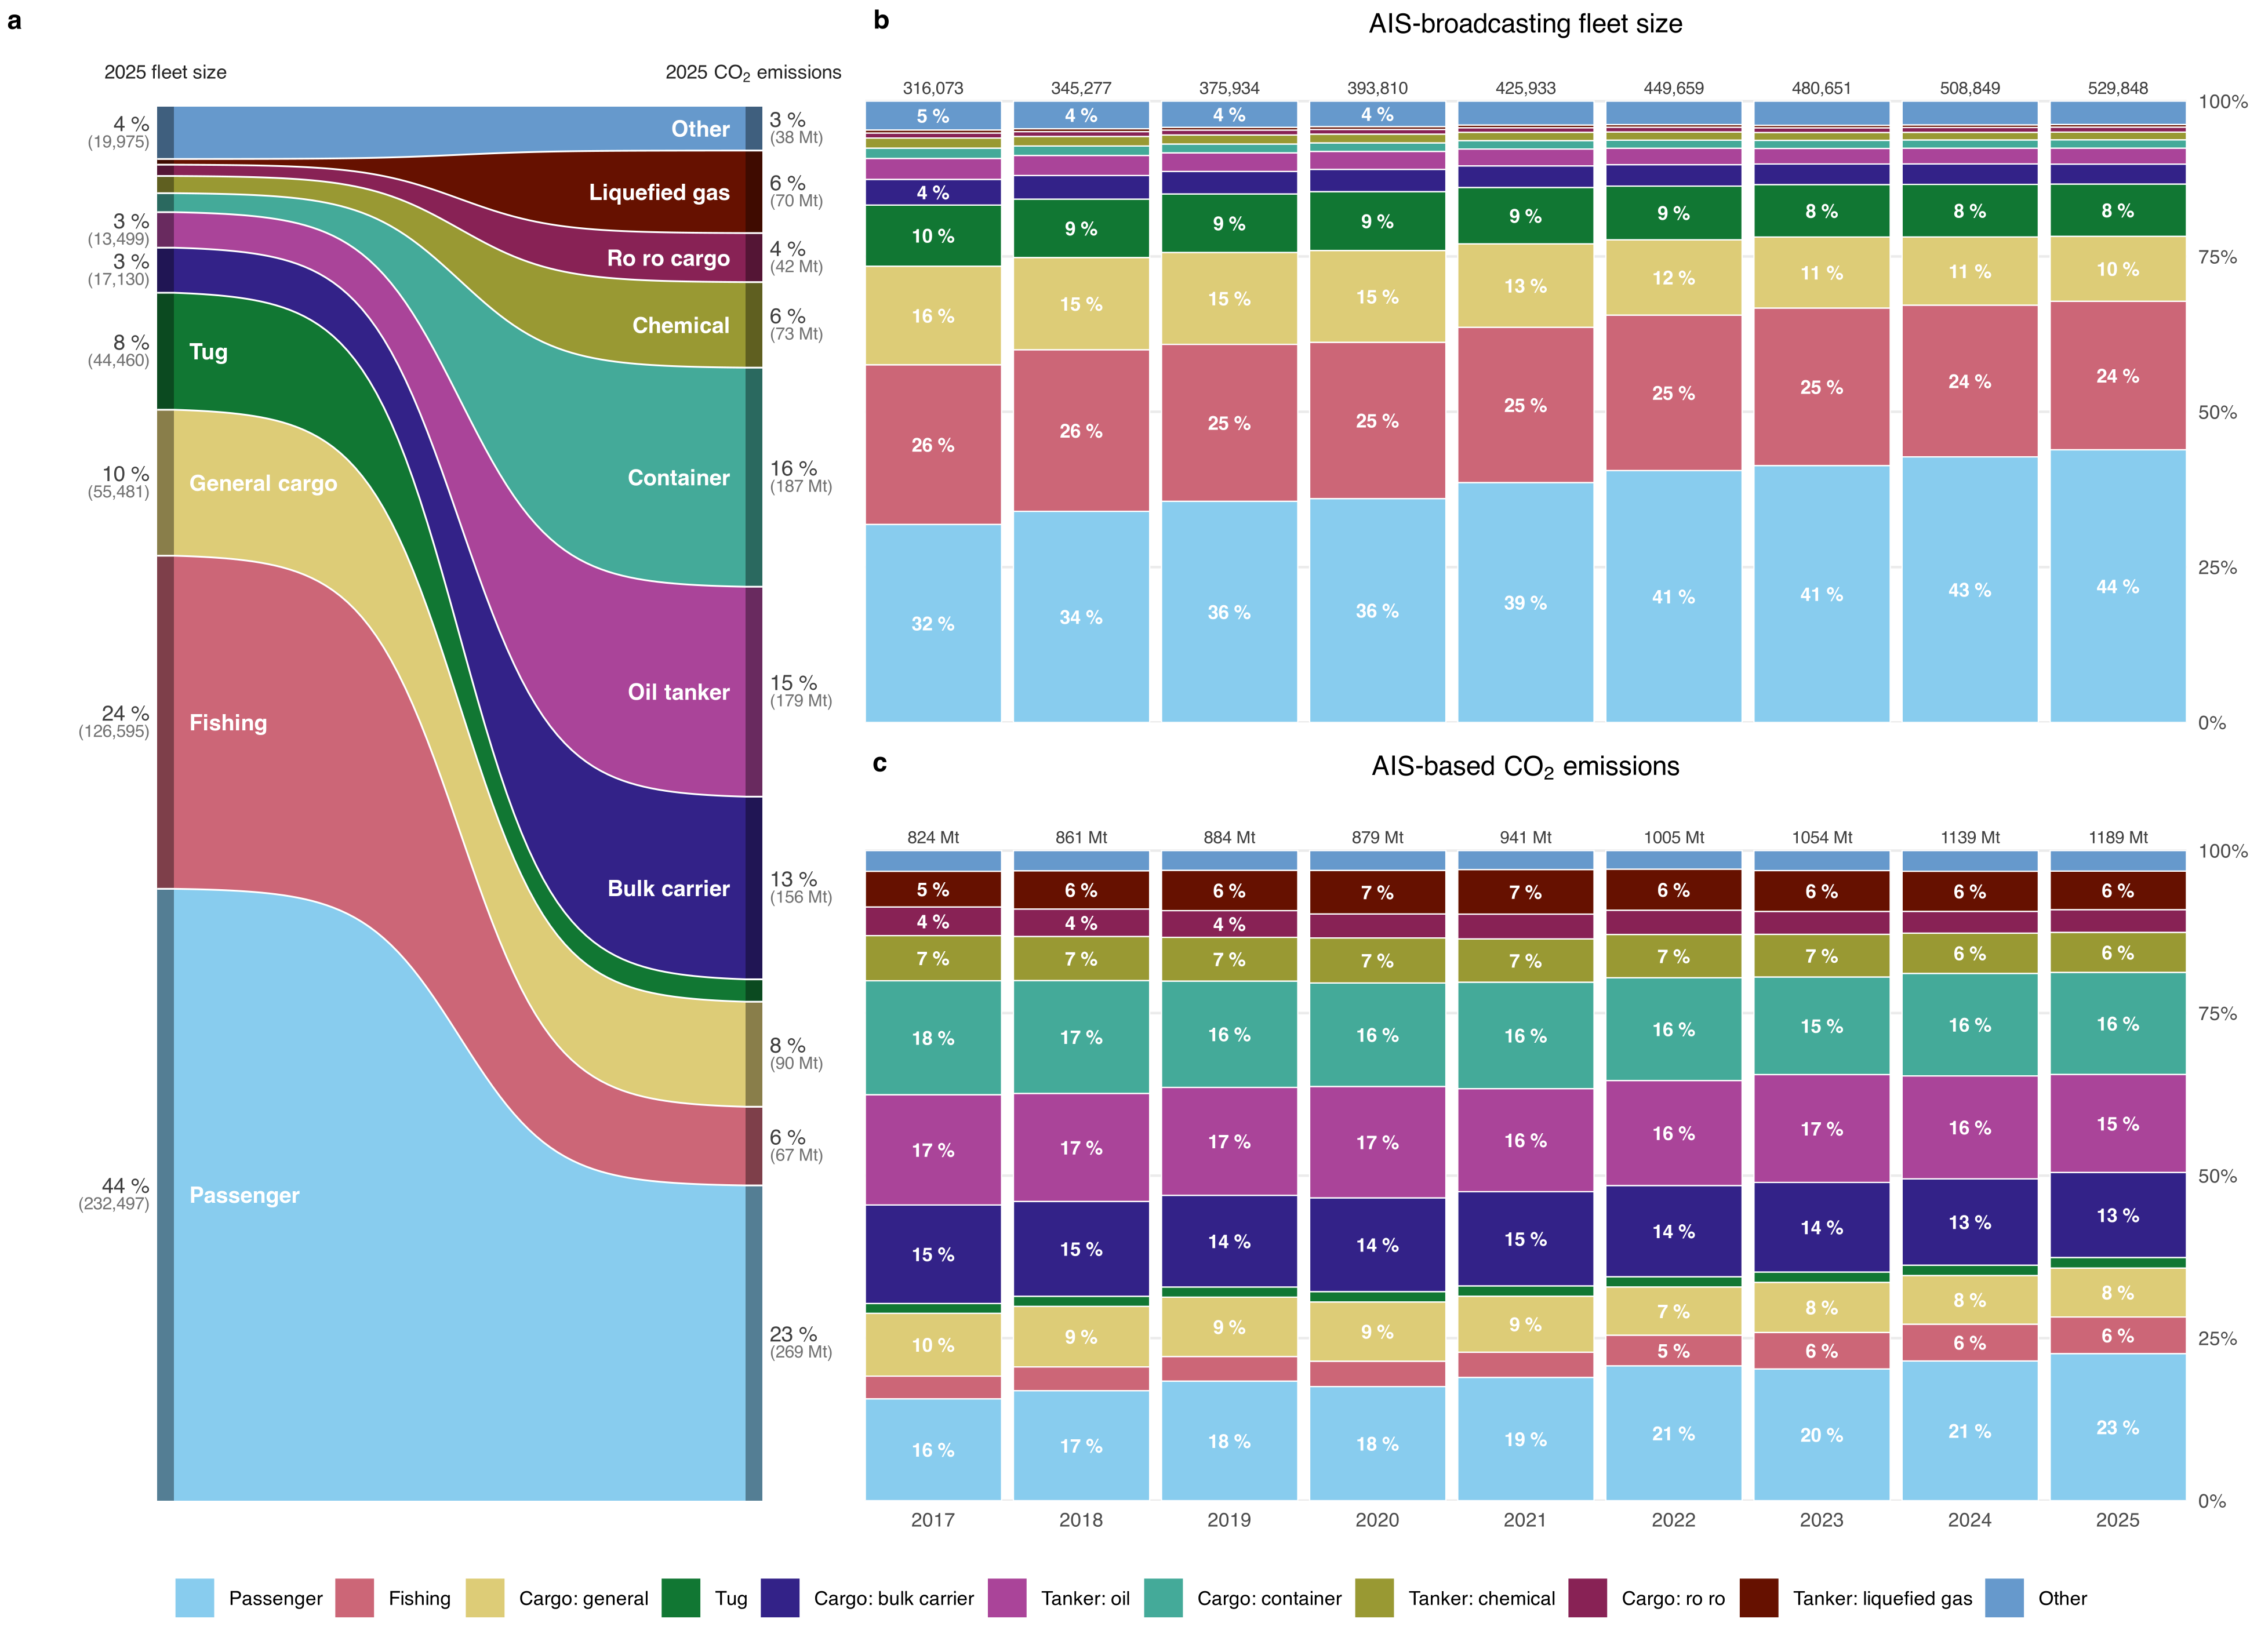
\includegraphics[width=\columnwidth]{figures/figS-fleet-sankey-with-series-2025-1.png}
    \caption{Fleet composition in 2025: each vessel class's share of the fleet against its share of CO$_{2}$, with the supporting series.}
    \label{fig:figS-fleet-sankey-with-series-2025}
\end{figure}

\section*{Supplementary Tables}

\begin{table}[!h]
\centering
\caption{\label{tab:total_percent_change_by_fleet}Summary of 2017 and 2025 emissions, data source and pollutant.}
\centering
\fontsize{6}{8}\selectfont
\setlength{\tabcolsep}{3pt}
\begin{tabular}[t]{l|l|l|l|l|l}
\hline
Source & Pollutant & \shortstack{2017\\emissions, MT} & \shortstack{2025\\emissions, MT} & \shortstack{Percent 2025\\total} & \shortstack{2017 to 2025\\change}\\
\hline
AIS-based & CO2 & 8.24e+08 & 1.19e+09 & 82\% & 44\%\\
\hline
S1-unmatched & CO2 & 2.41e+08 & 2.54e+08 & 18\% & 5\%\\
\hline
AIS-based + S1-unmatched & CO2 & 1.06e+09 & 1.44e+09 & 100\% & 36\%\\
\hline
AIS-based & CH4 & 11,500 & 15,800 & 84\% & 37\%\\
\hline
S1-unmatched & CH4 & 2,880 & 2,960 & 16\% & 3\%\\
\hline
AIS-based + S1-unmatched & CH4 & 14,400 & 18,700 & 100\% & 30\%\\
\hline
AIS-based & N2O & 41,800 & 59,500 & 83\% & 42\%\\
\hline
S1-unmatched & N2O & 11,800 & 12,400 & 17\% & 5\%\\
\hline
AIS-based + S1-unmatched & N2O & 53,600 & 71,900 & 100\% & 34\%\\
\hline
AIS-based & CO & 628,000 & 865,000 & 84\% & 38\%\\
\hline
S1-unmatched & CO & 160,000 & 165,000 & 16\% & 3\%\\
\hline
AIS-based + S1-unmatched & CO & 787,000 & 1,030,000 & 100\% & 31\%\\
\hline
AIS-based & NOX & 14,100,000 & 18,500,000 & 85\% & 31\%\\
\hline
S1-unmatched & NOX & 3,320,000 & 3,320,000 & 15\% & 0\%\\
\hline
AIS-based + S1-unmatched & NOX & 17,400,000 & 21,800,000 & 100\% & 25\%\\
\hline
AIS-based & SOX & 5,030,000 & 1,830,000 & 82\% & -64\%\\
\hline
S1-unmatched & SOX & 1,490,000 & 390,000 & 18\% & -74\%\\
\hline
AIS-based + S1-unmatched & SOX & 6,510,000 & 2,220,000 & 100\% & -66\%\\
\hline
AIS-based & PM2.5 & 701,000 & 590,000 & 84\% & -16\%\\
\hline
S1-unmatched & PM2.5 & 192,000 & 113,000 & 16\% & -41\%\\
\hline
AIS-based + S1-unmatched & PM2.5 & 893,000 & 703,000 & 100\% & -21\%\\
\hline
AIS-based & PM10 & 762,000 & 641,000 & 84\% & -16\%\\
\hline
S1-unmatched & PM10 & 208,000 & 123,000 & 16\% & -41\%\\
\hline
AIS-based + S1-unmatched & PM10 & 970,000 & 764,000 & 100\% & -21\%\\
\hline
AIS-based & VOCs & 641,000 & 868,000 & 85\% & 35\%\\
\hline
S1-unmatched & VOCs & 154,000 & 157,000 & 15\% & 2\%\\
\hline
AIS-based + S1-unmatched & VOCs & 795,000 & 1,020,000 & 100\% & 29\%\\
\hline
\end{tabular}
\end{table}

\FloatBarrier

\begin{table}[!h]
\centering
\caption{\label{tab:growth_share_by_family_length}Share of the 2017--2025 growth in AIS-based CO$_{2}$ emissions contributed by each vessel class family and length band. Each cell is that group's change in emissions as a share of the total change of 365 million metric tonnes (from 824 to 1,189 million), so the cells sum to 100\%. Vessel class families are as in Fig. \ref{fig:fig-ais-data-richness}; passenger vessels account for 38 of the 44 percentage points of the service and passenger family. Moving the upper length cutoff from 150 m to 200 m would shift 6 percentage points from the largest band to the middle band and leave the $<$50 m share unchanged. Percentages may not sum to totals because of rounding.}
\centering
\fontsize{7}{9}\selectfont
\begin{tabular}[t]{lrrrr}
\toprule
Vessel class family & $<$50 m & 50--150 m & $\geq$150 m & Total\\
\midrule
Cargo & 1\% & 2\% & 20\% & 24\%\\
Tanker & $<$1\% & 3\% & 19\% & 22\%\\
Service and passenger & 39\% & 4\% & 1\% & 44\%\\
Fishing & 10\% & 1\% & $<$1\% & 10\%\\
\midrule
Total & 50\% & 10\% & 40\% & 100\%\\
\bottomrule
\end{tabular}
\end{table}

\FloatBarrier

\begin{table}[!h]
\centering
\caption{\label{tab:growth_decomposition_by_family_length}Decomposition of the 2017--2025 change in AIS-based CO$_{2}$ emissions in each vessel class family and length band of Supplementary Table \ref{tab:growth_share_by_family_length}, in million metric tonnes. A cell's emissions are the product of its vessel count, the distance each vessel traveled (nm per vessel), and its emissions per nautical mile. The log-mean Divisia index \cite{angLMDIApproachDecomposition2005} splits the change in emissions exactly into a contribution from the change in each factor, so the three contributions in a row sum to its emissions change. Vessel count is the number of distinct AIS identities (MMSIs), so its change reflects fleet growth, the expansion of AIS carriage, and vessels changing MMSI. Among vessels of 150 m and over, MMSI changes make identities grow faster than physical hulls, so part of their vessel count contribution belongs to distance per vessel. Distance per vessel is observed distance, which also rises when improved AIS reception fills gaps in vessel tracks. Emissions per nautical mile include auxiliary engine and at-berth emissions, which accrue with time rather than distance, so this factor is not a measure of fuel efficiency alone.}
\centering
\fontsize{7}{9}\selectfont
\setlength{\tabcolsep}{3pt}
\begin{tabular}[t]{llrrrr}
\toprule
\multicolumn{3}{c}{ } & \multicolumn{3}{c}{Contribution from change in:} \\
\cmidrule(l{3pt}r{3pt}){4-6}
Vessel class family & Length & \shortstack{Emissions\\change} & \shortstack{Vessel\\count} & \shortstack{nm per\\vessel} & \shortstack{CO$_{2}$\\per nm}\\
\midrule
Cargo & $<$50 m & +3.9 & +1.4 & +0.2 & +2.3\\
 & 50--150 m & +8.8 & +11.5 & -7.0 & +4.4\\
 & $\geq$150 m & +74.3 & +86.9 & +4.0 & -16.7\\
\addlinespace
Tanker & $<$50 m & +0.9 & +0.4 & -0.2 & +0.7\\
 & 50--150 m & +10.8 & +7.9 & -5.1 & +8.0\\
 & $\geq$150 m & +68.9 & +94.1 & -21.1 & -4.1\\
\addlinespace
Service and passenger & $<$50 m & +142.2 & +126.3 & -23.3 & +39.2\\
 & 50--150 m & +14.1 & +10.9 & -0.8 & +4.0\\
 & $\geq$150 m & +3.1 & +6.4 & -3.5 & +0.2\\
\addlinespace
Fishing & $<$50 m & +35.0 & +15.3 & +13.5 & +6.2\\
 & 50--150 m & +3.2 & +0.3 & +0.8 & +2.1\\
 & $\geq$150 m & 0.0 & 0.0 & 0.0 & 0.0\\
\bottomrule
\end{tabular}
\end{table}

\FloatBarrier

\begin{table}[!h]
\centering
\caption{\label{tab:pollutant_ais_underestimation_overestimation_summary}Underestimation of 2025 emissions using only AIS data, and overestimation of the 2017 to 2025 percent change in emissions using only AIS data, by pollutant. Overestimation is the AIS-based percent change minus the AIS-based + S1-unmatched percent change, in percentage points; positive values mean AIS data alone show faster growth, or a slower decline, than the fused estimate.}
\centering
\fontsize{8}{10}\selectfont
\begin{tabular}[t]{l|l|l}
\hline
Pollutant & \shortstack{Underestimation of\\2025 emissions} & \shortstack{Overestimation of 2017-2025\\percent change (percentage points)}\\
\hline
CO2 & 18\% & 8.8\\
\hline
CH4 & 16\% & 7.0\\
\hline
N2O & 17\% & 8.3\\
\hline
CO & 16\% & 7.0\\
\hline
NOX & 15\% & 5.9\\
\hline
SOX & 18\% & 2.3\\
\hline
PM2.5 & 16\% & 5.4\\
\hline
PM10 & 16\% & 5.4\\
\hline
VOCs & 15\% & 6.5\\
\hline
\end{tabular}
\end{table}

\FloatBarrier

\begin{table}[!h]
\centering
\caption{\label{tab:emissions_by_ocean_summary_tbl}For each ocean, summary of: 2025 total (AIS+S1) CO$_2$ emissions (metric tonnes); percentage of global total (AIS+S1) 2025 CO$_2$ emissions from across all oceans; percent of 2025 total (AIS+S1) CO$_2$ emissions that are S1-unmatched; percent change in total (AIS+S1) CO$_2$ emissions from 2017 to 2025; and the percentage of all observations in the dataset (pixel-months) from 2017-2025 that were imaged by S1.}
\centering
\fontsize{7}{9}\selectfont
\setlength{\tabcolsep}{3pt}
\begin{tabular}[t]{l|l|l|l|l|l}
\hline
Summary statistic & Pacific & Atlantic & Indian & Arctic & Southern\\
\hline
2025 total CO2 emissions (million MT) & 457 & 449 & 222 & 4.13 & 0.567\\
\hline
Percent of total CO2 2025 emissions & 41.59\% & 38.98\% & 19.06\% & 0.32\% & 0.04\%\\
\hline
Percent of total CO2 emissions S1-unmatched & 20.60\% & 16.88\% & 16.10\% & 7.76\% & 0.00\%\\
\hline
Percent change in total CO2 emissions (2017 to 2025) & 44.17\% & 32.00\% & 28.48\% & 44.16\% & 263.43\%\\
\hline
Percent observations imaged by S1 (across 2017-2025) & 17.74\% & 35.94\% & 16.99\% & 13.55\% & 0.06\%\\
\hline
\end{tabular}
\end{table}

\FloatBarrier

\begin{table}[!h]
\centering
\caption{\label{tab:social_cost_summary_tbl}For both non-fishing vessels and fishing vessels, we summarize: the total emissions (metric tonnes) of each GHG gas; the social cost associated with each GHG (USD/metric tonne); the social cost of each (USD); the total social cost summed across all three gases (USD). We use 2021 for non-fishing vessels since it is the year for which we have the total value of all traded goods at sea. We use 2022 for fishing vessels since it is the year for which we have the total value of wild capture fisheries.}
\centering
\fontsize{8}{10}\selectfont
\begin{tabular}[t]{l|l|l|l|l|r}
\hline
Year & Vessel type & GHG & Emissions (MT) & SC (USD/MT) & SC (billion USD)\\
\hline
2021 & Non-fishing & CH4 & 14,397 & 2,900 & 0.042\\
\hline
2021 & Non-fishing & CO2 & 1,126,563,963 & 283 & 318.818\\
\hline
2021 & Non-fishing & N2O & 56,302 & 49,600 & 2.793\\
\hline
Total & Non-fishing & - & - & - & 321.652\\
\hline
2022 & Fishing & CH4 & 1,346 & 2,900 & 0.004\\
\hline
2022 & Fishing & CO2 & 81,011,499 & 283 & 22.926\\
\hline
2022 & Fishing & N2O & 4,127 & 49,600 & 0.205\\
\hline
Total & Fishing & - & - & - & 23.135\\
\hline
\end{tabular}
\end{table}

\FloatBarrier

\begin{table}[!h]
\centering
\caption{\label{tab:top_countries_by_activity_type}Top 30 countries by 2025 CO$_{2}$ emissions (millions of metric tonnes) from AIS-broadcasting vessels, shown separately for each activity type, with all remaining countries pooled into a single Other row. Emissions for each international trip are partitioned equally to its departure and arrival country. These are the totals mapped in Figure \ref{fig:fig-emissions-by-country-and-activity-type}.}
\centering
\fontsize{7}{9}\selectfont
\begin{tabular}[t]{lrlrlr}
\toprule
\multicolumn{2}{c}{International trips} & \multicolumn{2}{c}{Port stays} & \multicolumn{2}{c}{Domestic trips} \\
\cmidrule(l{3pt}r{3pt}){1-2} \cmidrule(l{3pt}r{3pt}){3-4} \cmidrule(l{3pt}r{3pt}){5-6}
Country & CO$_{2}$ & Country & CO$_{2}$ & Country & CO$_{2}$\\
\midrule
China & 55.5 & China & 74.2 & China & 66.8\\
Malaysia & 48.1 & United States & 27.9 & Japan & 13.1\\
United States & 39.9 & Indonesia & 10.6 & United States & 13.1\\
South Korea & 20.2 & Spain & 9.8 & Indonesia & 8.8\\
Australia & 19.1 & South Korea & 9.0 & South Korea & 5.7\\
\addlinespace
Brazil & 18.9 & Netherlands & 9.0 & Russia & 5.6\\
Spain & 15.7 & Japan & 8.9 & Norway & 5.4\\
Japan & 15.5 & United Arab Emirates & 8.4 & Brazil & 5.2\\
India & 15.2 & Norway & 8.4 & Australia & 3.8\\
United Arab Emirates & 14.2 & Italy & 8.1 & Malaysia & 3.4\\
\addlinespace
Panama & 13.8 & Australia & 7.6 & India & 3.4\\
Singapore & 12.7 & Turkey & 7.4 & Italy & 3.2\\
Egypt & 10.4 & France & 7.2 & Spain & 3.1\\
Indonesia & 9.0 & United Kingdom & 6.7 & Turkey & 2.7\\
Russia & 8.5 & Germany & 6.0 & United Kingdom & 2.6\\
\addlinespace
United Kingdom & 7.7 & Greece & 5.8 & Canada & 2.5\\
Netherlands & 7.4 & Brazil & 5.3 & Vietnam & 2.3\\
Canada & 6.9 & Russia & 5.0 & United Arab Emirates & 2.2\\
Mexico & 6.4 & India & 4.8 & Philippines & 2.2\\
Turkey & 6.3 & Malaysia & 4.7 & Greece & 1.8\\
\addlinespace
Taiwan & 6.1 & Canada & 4.5 & Taiwan & 1.8\\
Belgium & 6.0 & Denmark & 4.4 & France & 1.7\\
France & 5.6 & Belgium & 3.9 & Egypt & 1.7\\
Saudi Arabia & 5.5 & Saudi Arabia & 3.3 & Saudi Arabia & 1.6\\
South Africa & 5.5 & Mexico & 2.8 & Mexico & 1.3\\
\addlinespace
Vietnam & 5.4 & Thailand & 2.8 & Germany & 1.1\\
Italy & 5.0 & Sweden & 2.5 & Chile & 1.1\\
Germany & 5.0 & Philippines & 2.3 & Thailand & 1.1\\
Sri Lanka & 4.9 & Taiwan & 2.2 & New Zealand & 1.0\\
Morocco & 4.7 & Egypt & 2.2 & Argentina & 1.0\\
\addlinespace
Other & 107.2 & Other & 59.3 & Other & 19.5\\
\bottomrule
\end{tabular}
\end{table}

\FloatBarrier


\section*{Supplementary Notes}

\supnote{Trends in AIS receiver types}{sec:ais-receiver-types}

AIS messages are broadcast from vessels and then received through one of three technologies: satellite-based receivers, terrestrial receivers, and dynamic receivers. Satellite and terrestrial receivers are the oldest receiver types, while 2022 saw the widespread adoption of dynamic AIS (D-AIS) in several regions throughout the world. D-AIS is a technology that was first implemented by Spire, one of the major AIS data providers, in which satellite-enabled AIS receivers are installed on vessels that travel through some of the world's busiest shipping lanes, such as the South China Sea \cite{spire_documentation_2022}. Through GFW, we can determine the receiver type for every single AIS message in the dataset over time. In Supplementary Fig. \ref{fig:fig-annual-emissions-by-ais-receiver-type}, we summarize the amount of estimated emissions and the number of distinct vessels that were detected by the three different types of AIS receivers. In 2022, we can clearly see a sharp rise in the amount of emissions that were estimated from D-AIS, which coincides with a decrease in the emissions that are estimated from satellite and terrestrial receivers. In aggregate, this led to an increase in total estimated emissions. The number of distinct vessels detected by D-AIS also sharply rose in 2022, almost equaling the number of vessels detected by all receiver types.

\begin{figure}[H]
    \centering
    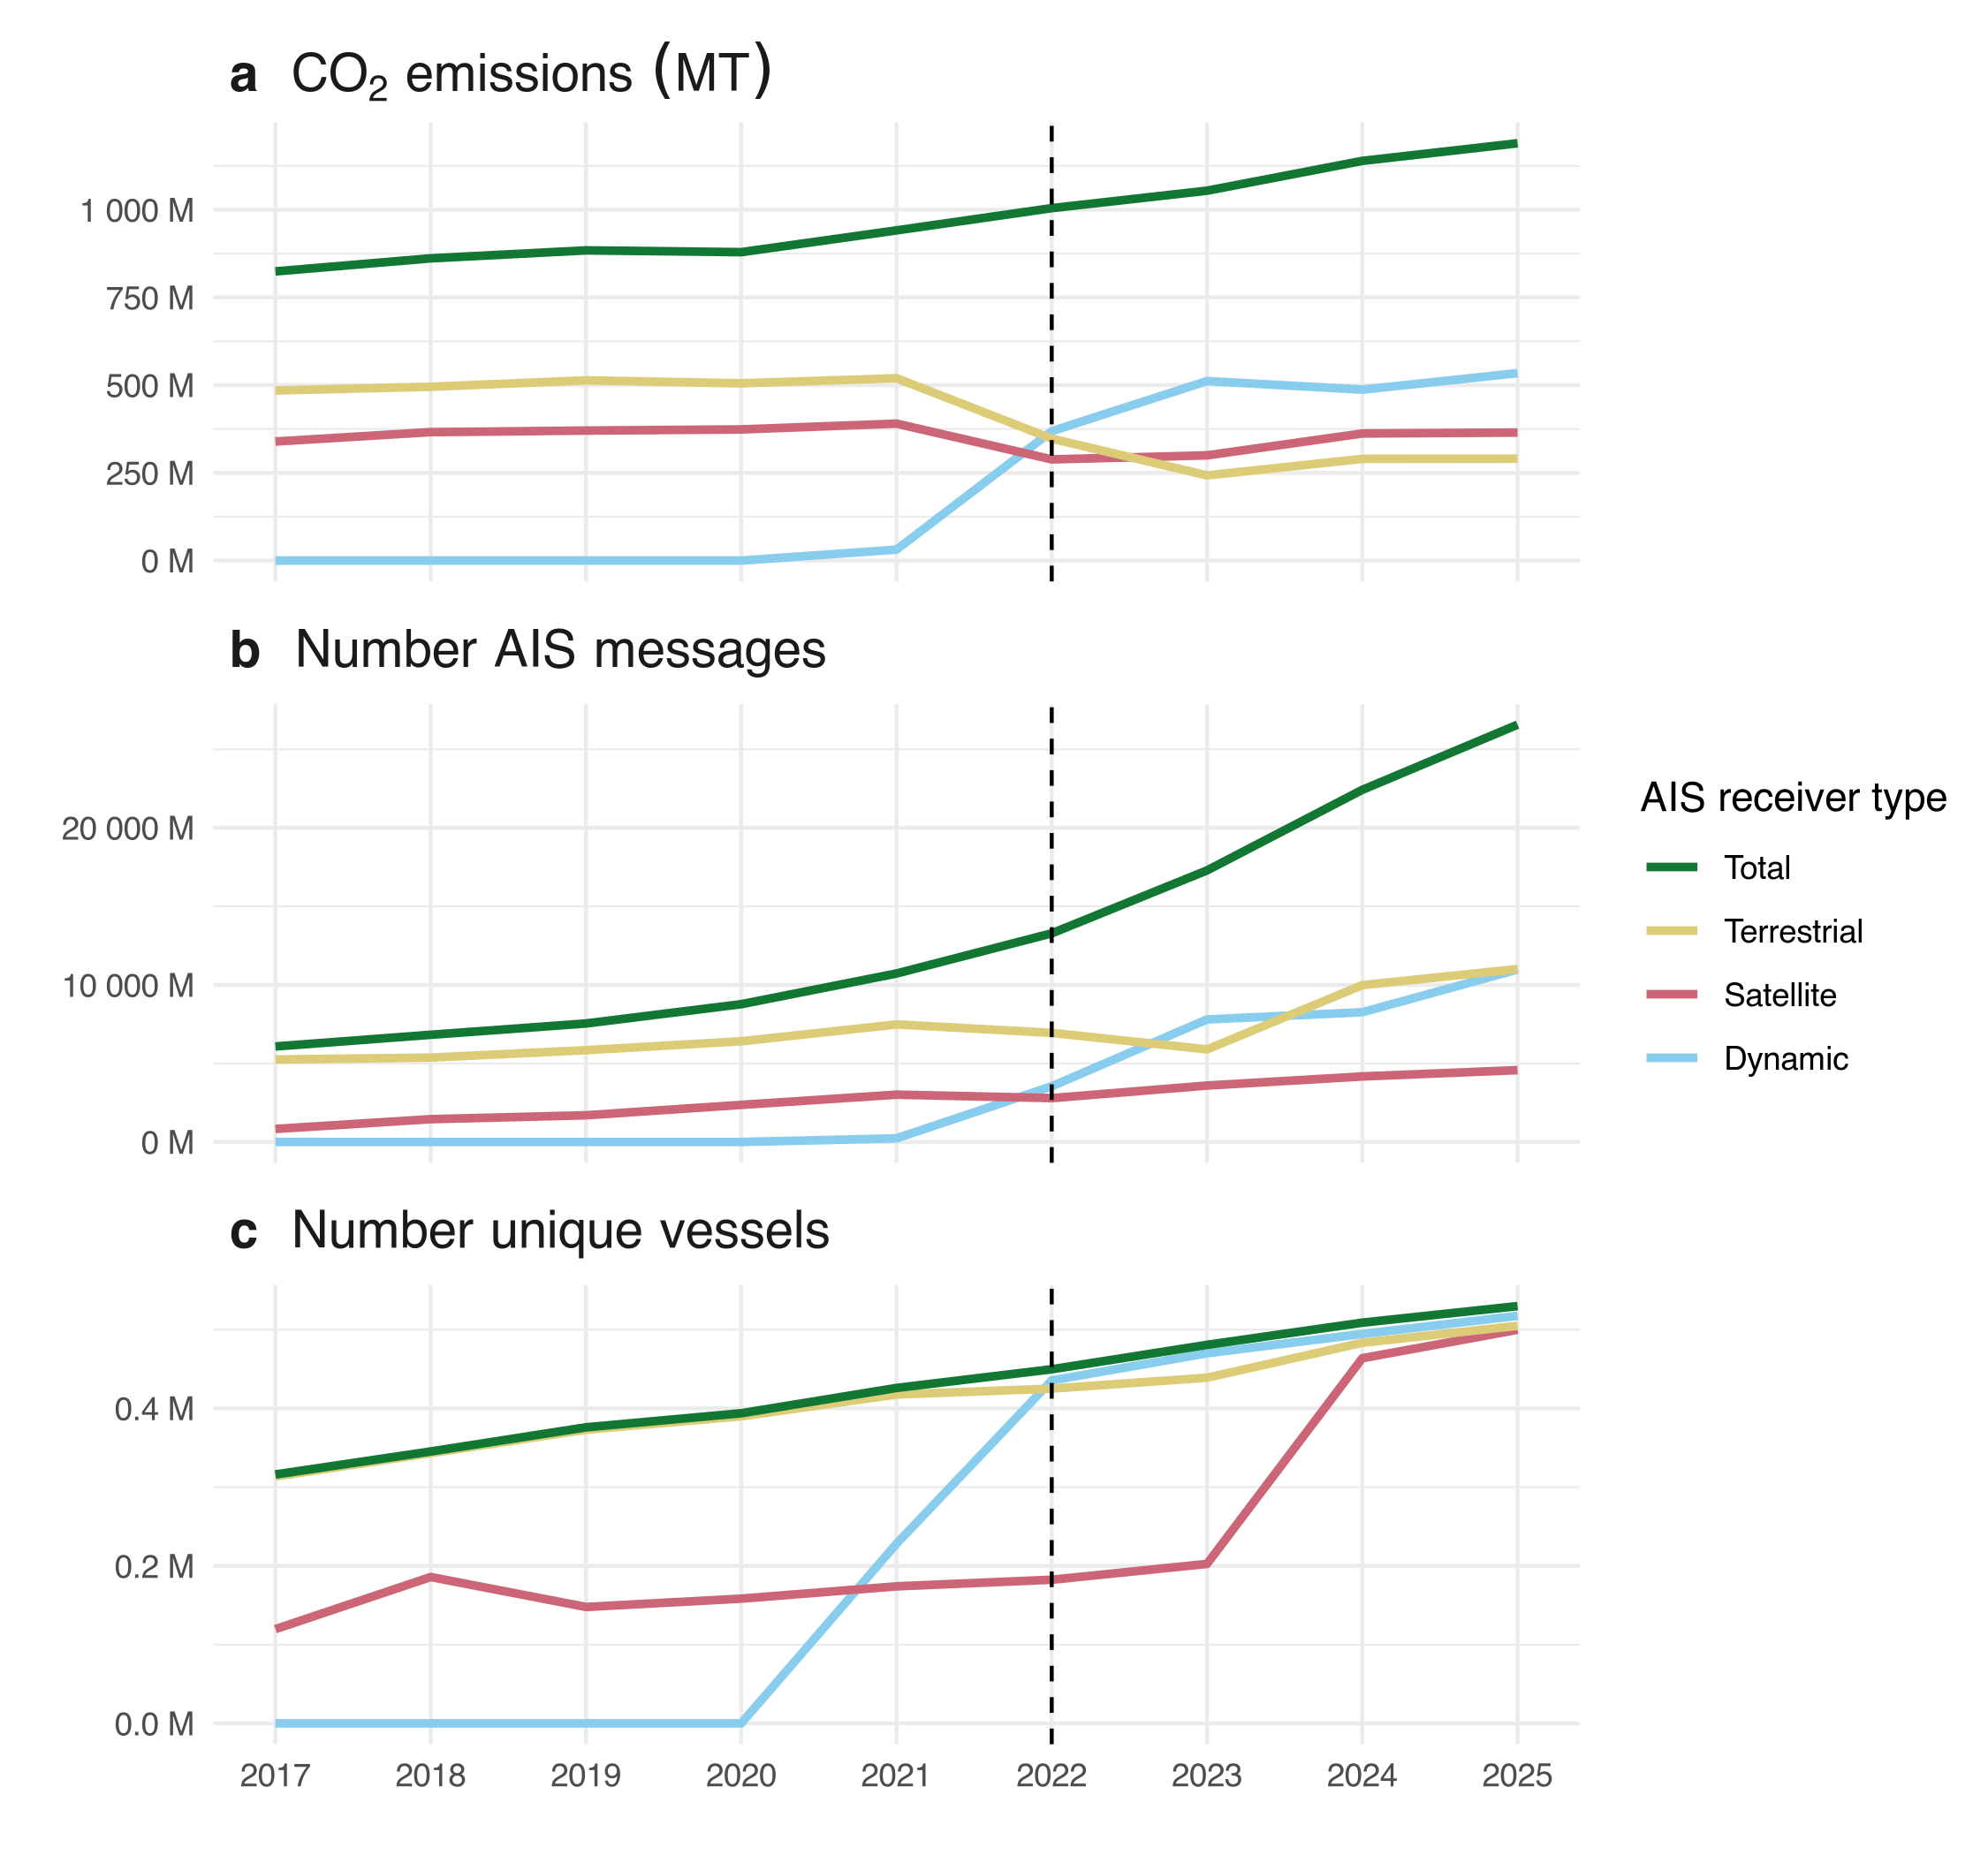
\includegraphics[width=\columnwidth]{figures/fig-annual-emissions-by-ais-receiver-type-1.png}
    \caption{(a) Annual total CO$_{2}$ emissions (metric tonnes) by AIS-broadcasting vessels, (b) AIS pings (i.e., individual vessel timestamped location messages), and (c) number of unique AIS-broadcasting vessels. Trends are disaggregated by AIS receiver type (satellite, terrestrial, and dynamic), and also shown as a total aggregated across receiver types. A dashed vertical line is shown for 2022, the first year in which D-AIS was widely adopted.}
    \label{fig:fig-annual-emissions-by-ais-receiver-type}
\end{figure}

In Supplementary Fig. \ref{fig:fig-annual-emissions-by-ais-receiver-type-top-flags}, we see the amount of quantified emissions for the top 10 vessel flags broken apart by AIS receiver type. The trends are similar to those seen in aggregate (Supplementary Fig. \ref{fig:fig-annual-emissions-by-ais-receiver-type}), although there is variation in terms of the increase in D-AIS detections across different flags. This is likely driven by whether vessels of each flag travel through regions where D-AIS was widely adopted. It is important to note that toward the end of 2021, China experienced a blackout of terrestrial AIS signals due to new privacy laws that were being implemented \cite{benefits_dynamic_ais}.

\begin{figure}[H]
    \centering
    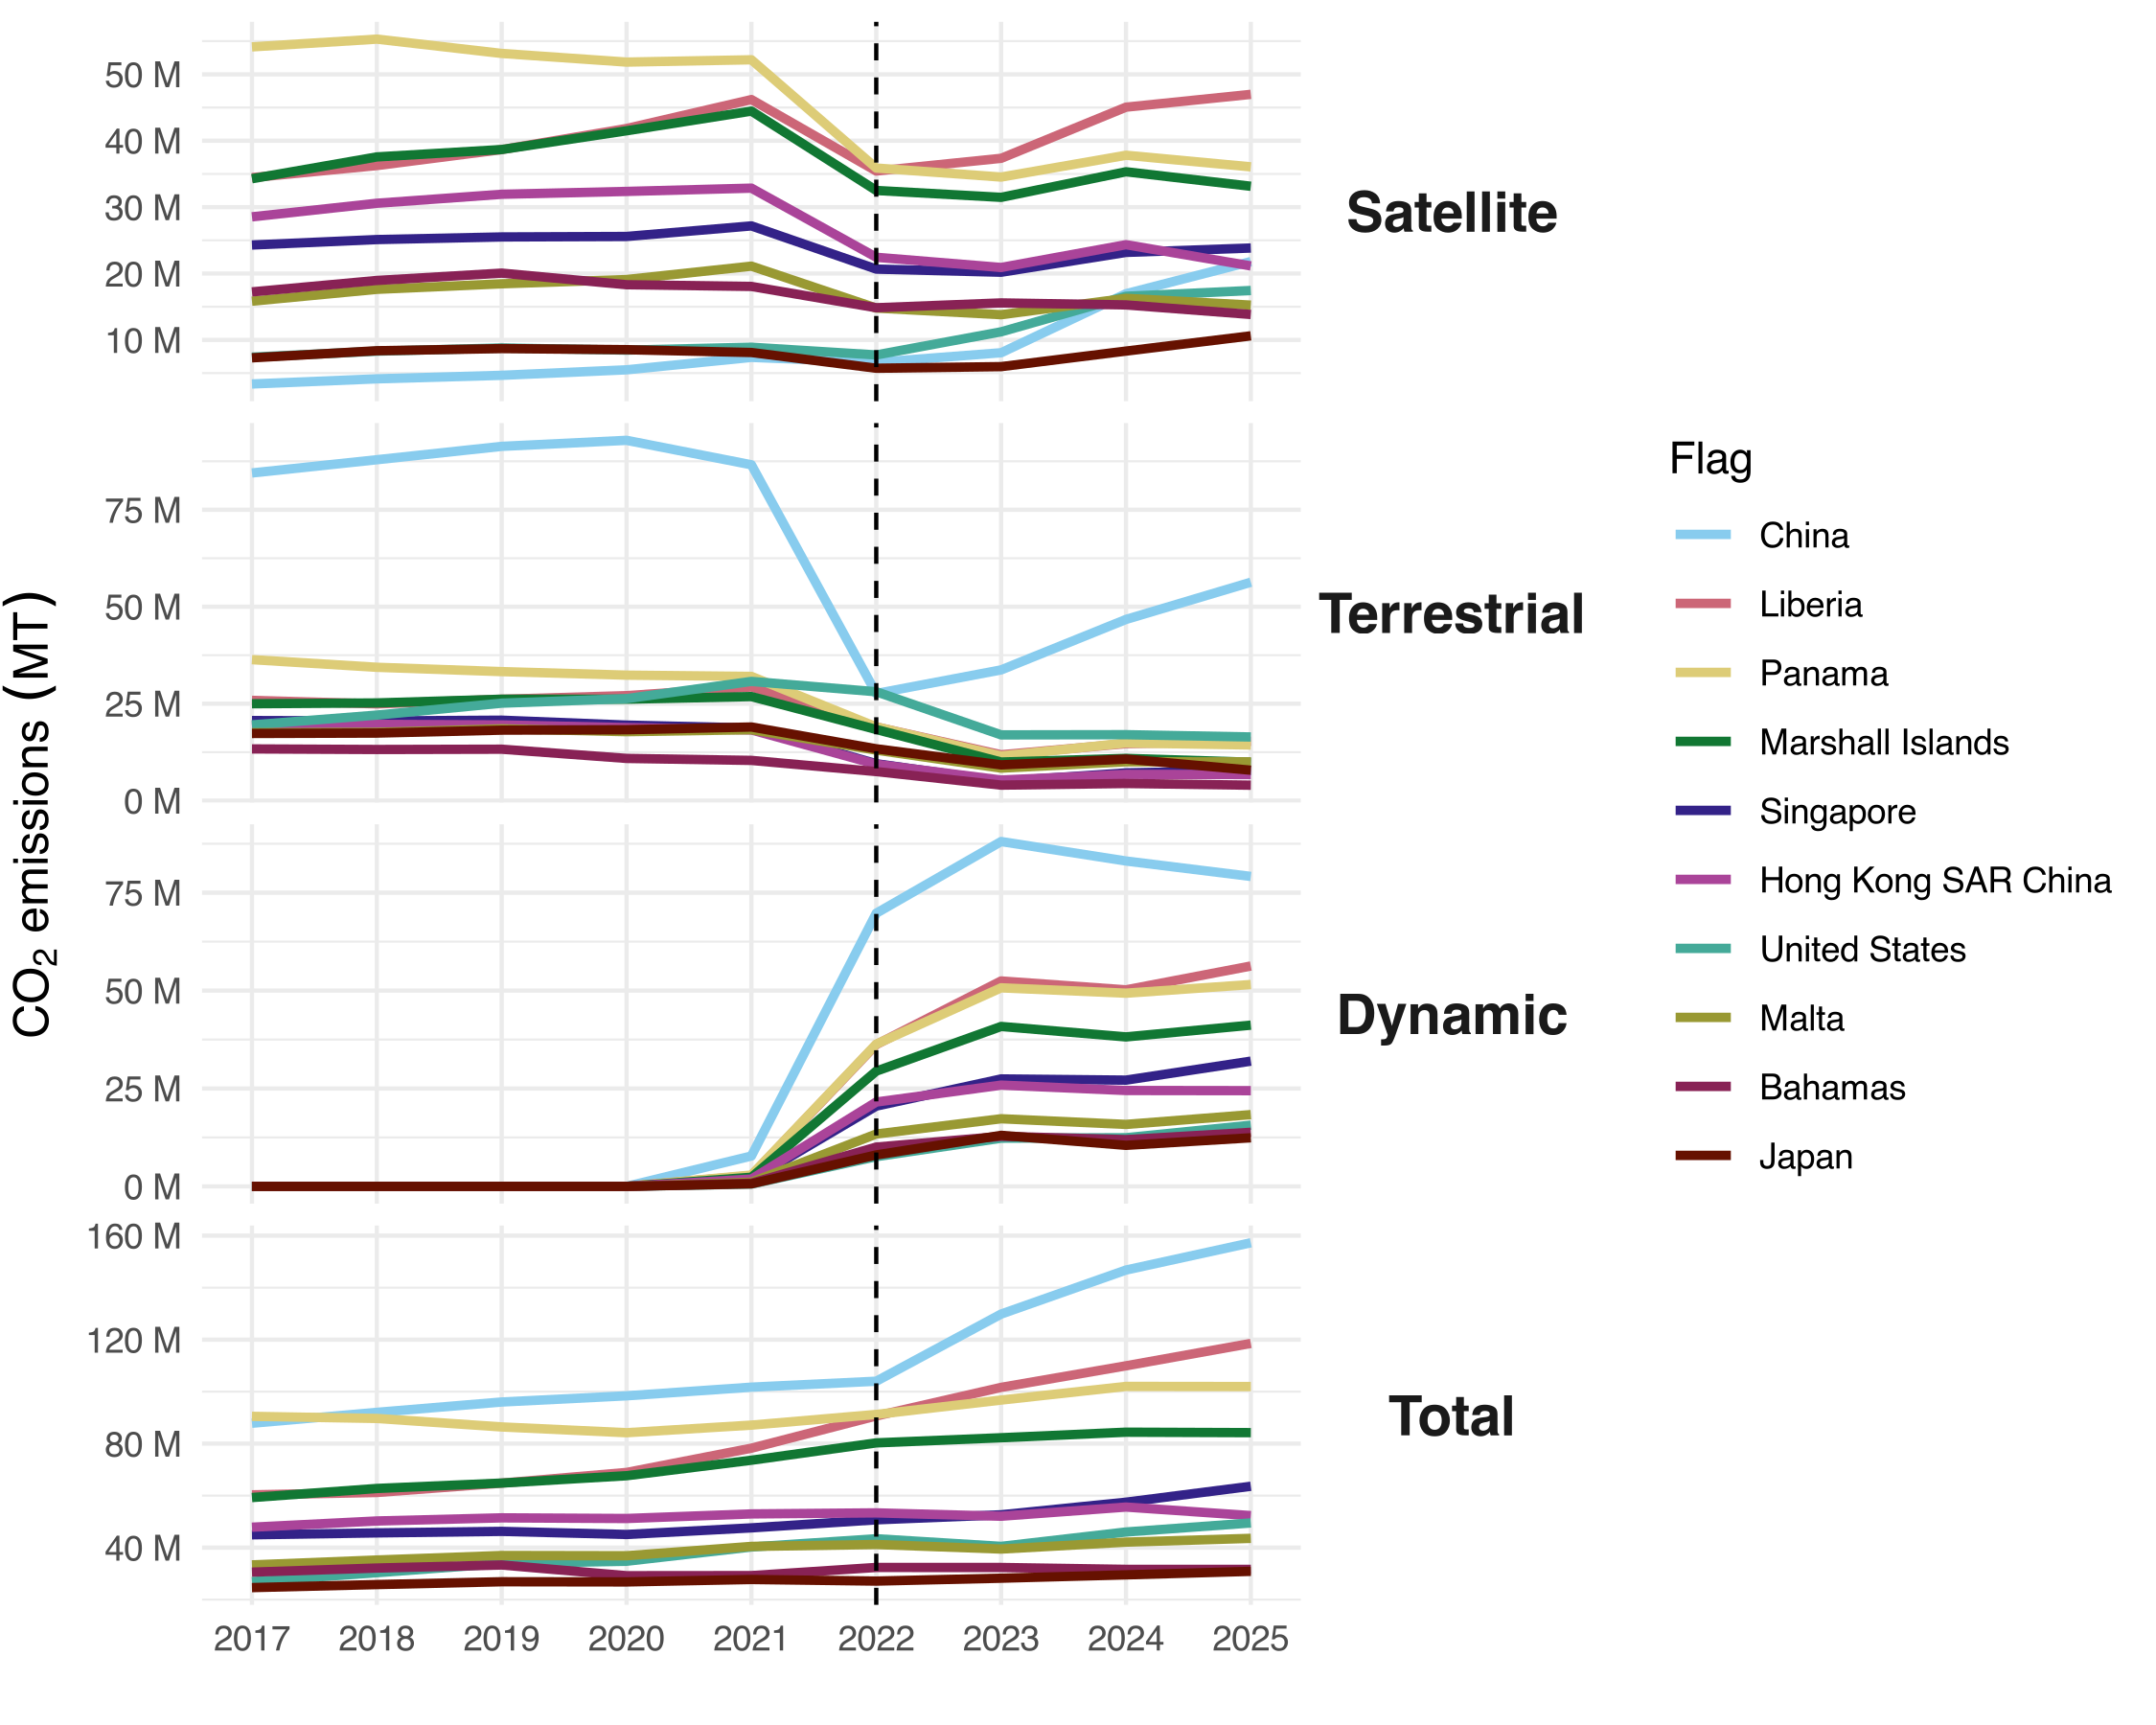
\includegraphics[width=\columnwidth]{figures/fig-annual-emissions-by-ais-receiver-type-top-flags-1.png}
    \caption{Annual total CO$_{2}$ emissions (metric tonnes) by AIS-broadcasting vessels, disaggregated by AIS receiver type (satellite, terrestrial, and dynamic) and total aggregated across receiver types, for the top 10 flags with the most emissions in 2025. A dashed vertical line is shown for 2022, the first year in which D-AIS was widely adopted.}
    \label{fig:fig-annual-emissions-by-ais-receiver-type-top-flags}
\end{figure}

Finally, in Supplementary Fig. \ref{fig:fig-co2-emissions-change-map-by-receiver-type}, we see how the use of the three AIS receiver types has changed spatially over time between 2017 and 2025. D-AIS was mostly implemented in busy shipping lanes, with clear concentration in areas including the South China Sea, Europe, and the Gulf of Mexico. These regions also generally correspond to decreasing use of satellite and terrestrial receivers. Overall, the largest total change in emissions is generally concentrated in the same regions that saw the largest uptake of D-AIS.

\begin{figure}[H]
    \centering
    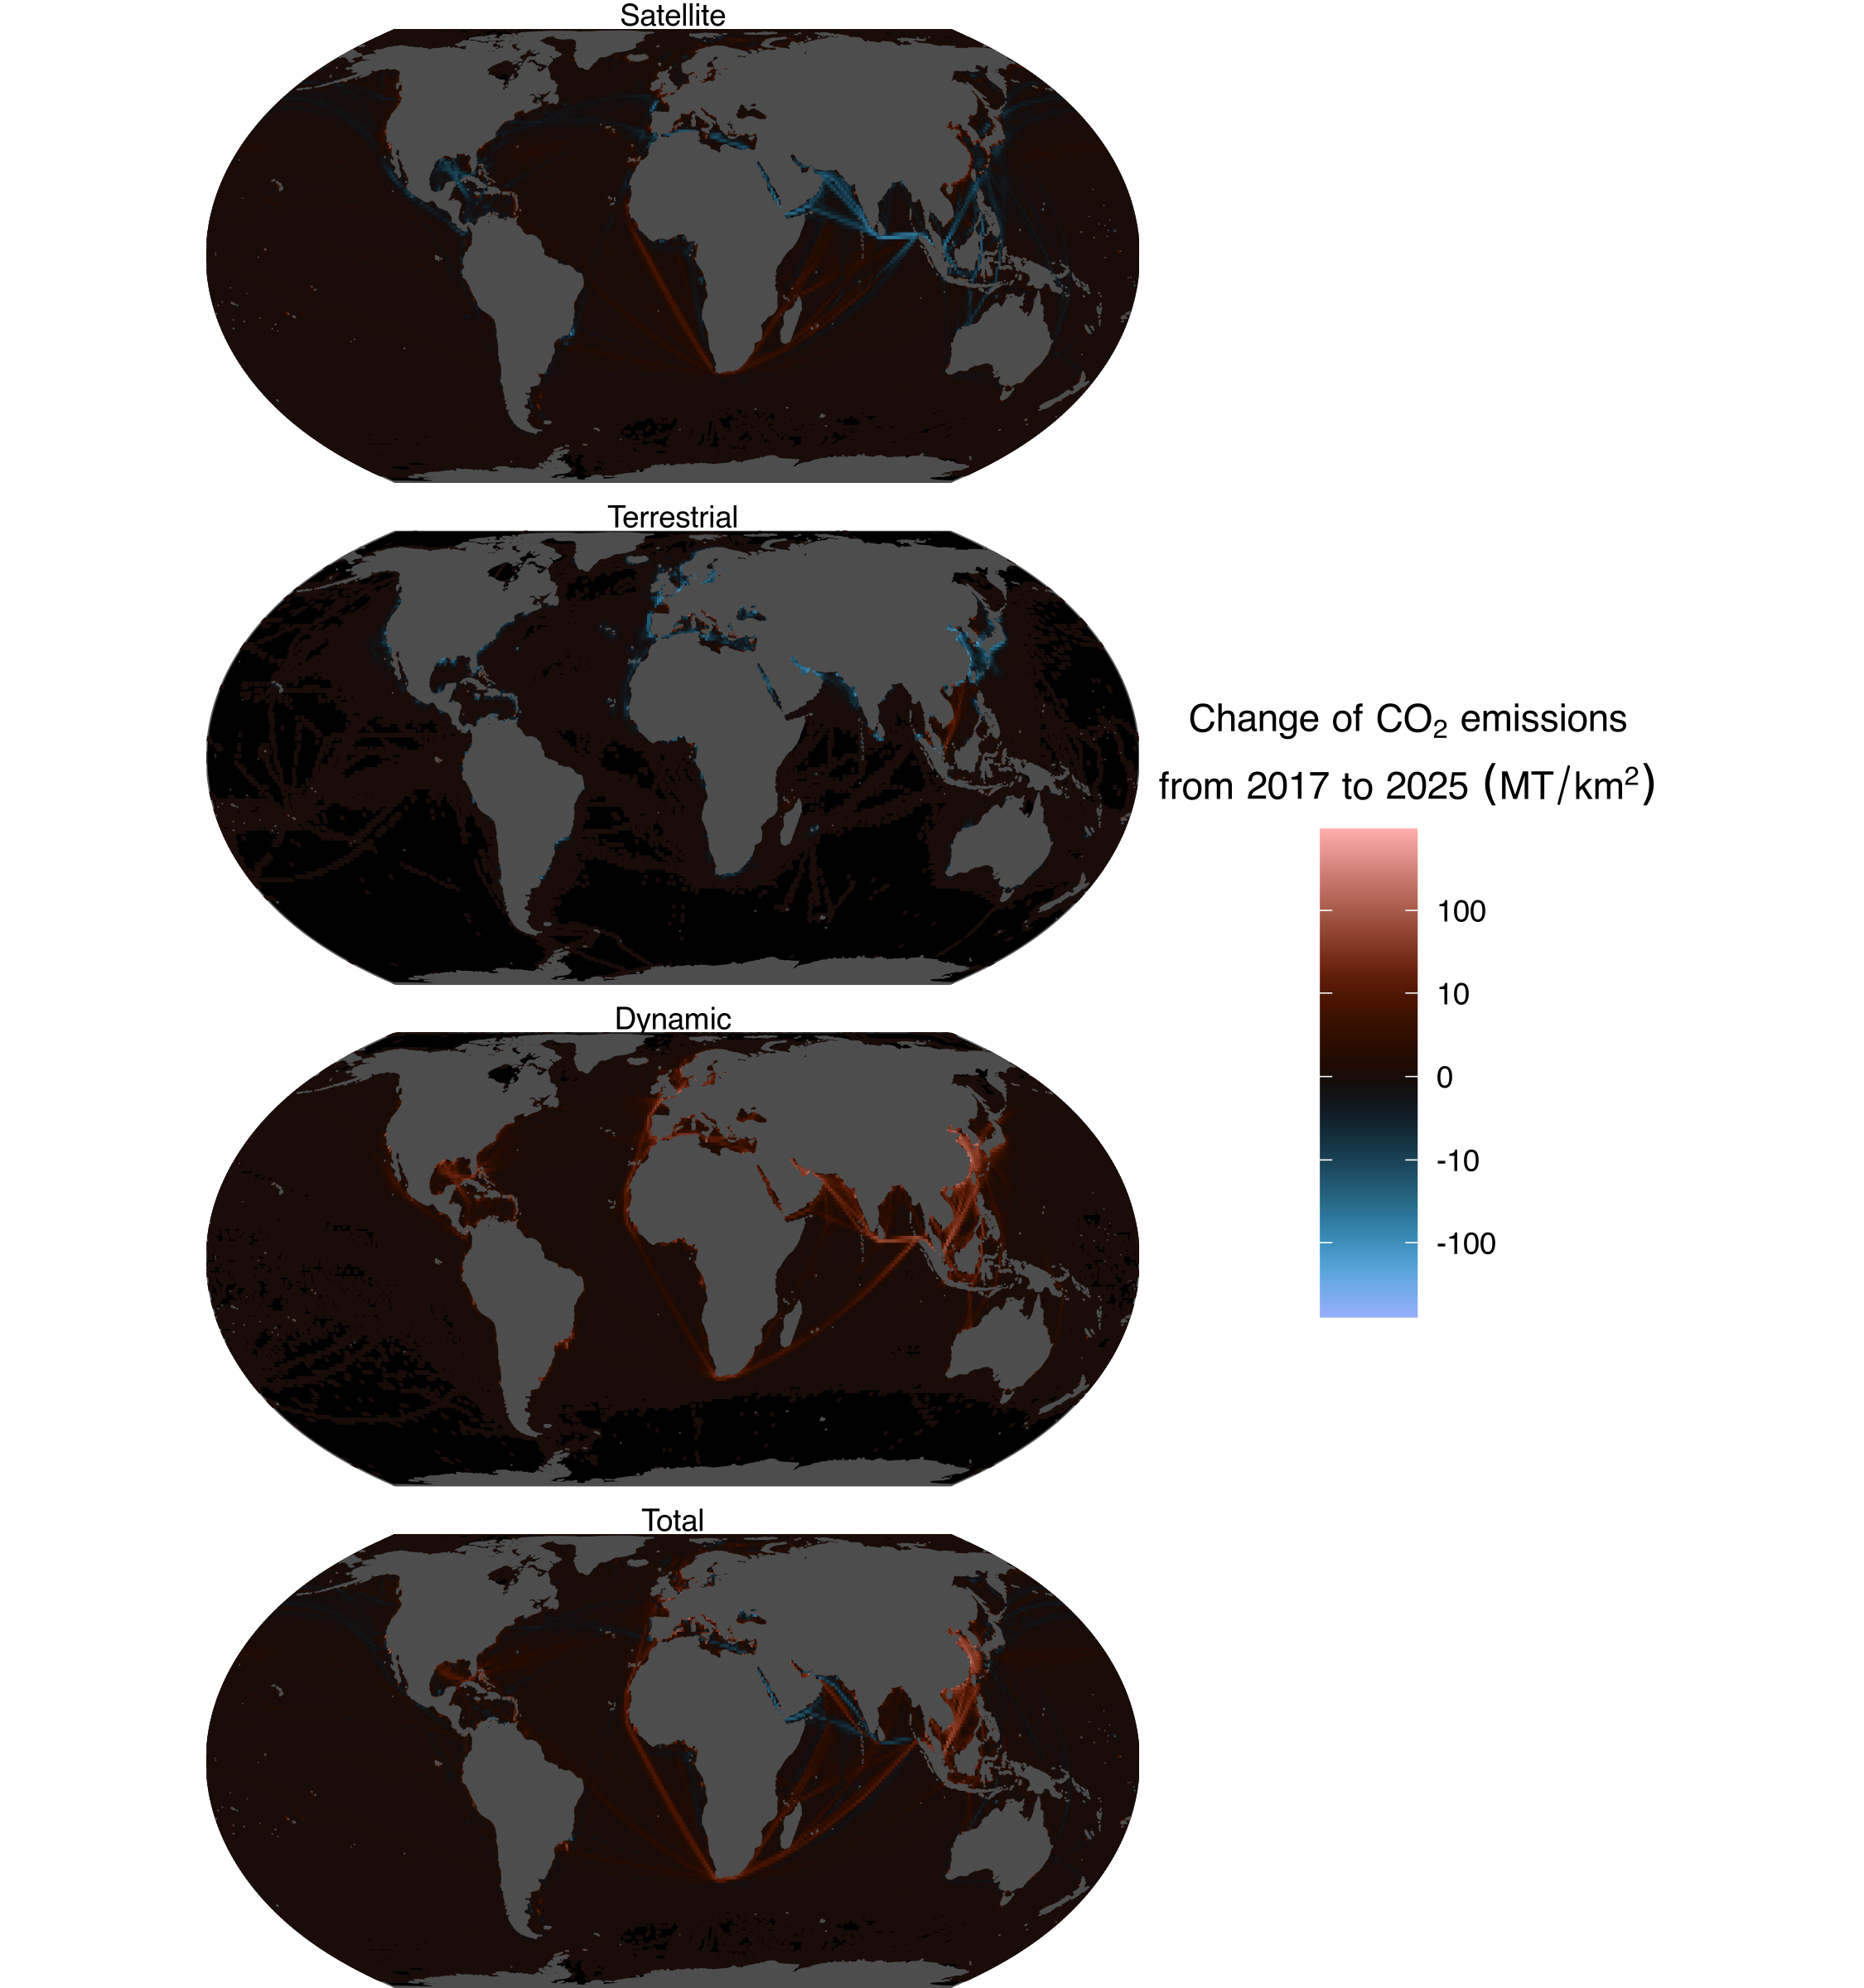
\includegraphics[width=\columnwidth]{figures/fig-co2-emissions-change-map-by-receiver-type-1.png}
    \caption{Spatial change in CO$_{2}$ emissions by AIS-broadcasting vessels between 2017 and 2025 (metric tonnes) by receiver type (satellite, terrestrial, and dynamic) and total across receiver types, at a 1x1 degree spatial resolution; emissions are area-normalized for each pixel (metric tonnes per square kilometer, shown on a pseudolog-10 scale).}
    \label{fig:fig-co2-emissions-change-map-by-receiver-type}
\end{figure}


\supnote{Systematic comparison of our AIS-based emissions modeling methodology to other AIS-based inventories}{sec:methods-comparison}

\subsubsection*{Scope of the comparison and modeling approaches}

Global vessel emission estimates fall into two methodological families, distinguished by whether emissions are derived from aggregate country-level fuel use statistics (i.e., `top-down') or from the observed activity of individual vessels (i.e., `bottom-up'). Top-down, fuel-based inventories combine reported marine fuel sales with fleet-wide emissions factors, without using data on individual vessels. They are unable to estimate vessel-level emissions or assign emissions with high spatiotemporal precision, and are known to underestimate emissions relative to activity-based inventories \cite{miolaEstimatingAirEmissions2011}. Bottom-up, activity-based approaches instead derive emissions mechanistically from the observed movement of individual vessels, calculating the pollutants emitted by each vessel in a specific spatial context and aggregating over time and fleet \cite{nunesActivitybasedMethodologyAssess2017}. 

Since the widespread adoption of AIS, which resolves vessel activity and operational mode at high spatial and temporal resolution, bottom-up AIS-based models have become the reference methodology for global inventories and the approach adopted by the IMO \cite{fourth2020greenhouse}. We therefore build on an extensive body of work and literature that has been developed over the last several decades. The most recent and representative global bottom-up inventories include:

\begin{itemize}
    \item Ship Traffic Emissions Assessment Model (STEAM) \cite{jalkanen2009modelling, jalkanenExtensionAssessmentModel2012, bergShipEmissionsSO22012, johanssonGlobalAssessmentShipping2017, majamaki2025improving}
    \item Shipping Emission Inventory Model (SEIM) \cite{wangShipEmissionsChina2021, yiHighresolutionGlobalShipping2025}
    \item Maritime Transport Environmental Assessment Model (MariTEAM) \cite{kramelGlobalShippingEmissions2021}
    \item the OECD's latest bottom-up model update (hereafter `OECD') \cite{clarke2023co2, oecdMaritimeTransportCO2Methodology2025}
    \item the SAVE model developed by the ICCT (hereafter `SAVE') \cite{olmer2017greenhouse, documentationV2025031Documentation, mao2025greenhouse}, and
    \item the model used for the Fourth IMO GHG Study (`IMO' in figures and tables) \cite{fourth2020greenhouse}.

\end{itemize}

In the following sections, we compare our AIS-based emissions model to each of these existing inventories. Any AIS-based inventory is assembled from four components, and the differences between these components affect the scope, resolution, and accuracy of each inventory. First, the AIS record itself, which determines which vessels and which movements are observed at all. Second, a vessel-characteristics dataset supplying the parameters the model requires. Third, an engine model converting observed speed into instantaneous main engine load, plus assumptions on auxiliary engine and boiler demand. Fourth, fuel consumption and pollutant-specific emission factors, conditioned on engine type, fuel type and the regulation in force at the time and place of the emission. Supplementary Data 1, 2 and 3 compare our methods, input data, and outputs, respectively, against each of the inventories listed above. We end with a comparison of how each inventory is validated against external data sources, and what this tells us about the accuracy of each inventory.

\subsubsection*{Activity and vessel-characteristics data}

All seven inventories are global in spatial extent, so the differences lie in AIS coverage, fleet size, and temporal coverage rather than in geographic scope (Supplementary Data 2). The inventories diverge substantially in the number of vessels represented. Restricting the comparison to vessels explicitly modeled from observed AIS activity, we model 800,670 unique vessels over 2015--2025 (a wider window, and so a larger fleet, than the 775,358 vessels emitting during the 2017--2025 study period used elsewhere in this paper), an average of 396,221 vessels per year rising from 249,732 in 2015 to 529,848 in 2025. This exceeds the AIS-modeled fleet of the Fourth IMO GHG Study, OECD, SAVE, MariTEAM and SEIM. Only STEAM reports a comparable fleet: 376,219 vessels in 2015, more than our 249,732 in that year. However, STEAM does not report fleet sizes in subsequent updates, preventing a direct comparison for the later years in which our fleet is larger.

The difference with STEAM is also reflected in the underlying AIS data, which used approximately 7.8 billion AIS positions in 2015, compared with approximately 2.3 billion in our 2015 dataset after data cleaning. Our own message volume increases to approximately 26.6 billion positions by 2025, totaling approximately 125 billion positions over 2015--2025 (an average of 11.4 billion per year), reflecting the expansion of terrestrial and satellite AIS. Among the remaining inventories, SEIM and MariTEAM report lower AIS message volumes, and the others do not indicate message counts. The increase in AIS messages also reflects the differences in the AIS data types available to us. Terrestrial and satellite AIS constitute the core AIS data types. In addition, GFW obtains a data add-on for both class A and class B D-AIS (also marketed as shipborne AIS), released by the data provider Spire since 2022, which further increases the density and coverage of our AIS record. To our knowledge, D-AIS is generally not included in base AIS data products from most providers, and the inventories covering 2022 onward report conventional AIS data types without indicating whether D-AIS is included, so we cannot determine whether the differences arise from the input data or from a lack of reporting. Of the inventories compared, only OECD (2019 onward) and SAVE (2016-2023) extend into the D-AIS era at all; STEAM's update ends in 2021, SEIM in 2021, the Fourth IMO GHG Study in 2018, and MariTEAM is a single-year 2017 inventory. The question of whether D-AIS inflates our recent trend relative to the others therefore applies to two of the six comparisons. 

Temporal coverage differs in extent. STEAM and MariTEAM are single-year inventories (2015 and 2017 respectively), with STEAM subsequently updated through 2021 to account for ambient conditions \cite{majamaki2025improving}. SEIM covers 2013 and 2016--2021, the Fourth IMO GHG Study 2012--2018, SAVE 2016--2023, and OECD from 2019 onward. Our use of consistent GFW AIS products, though input density evolves, enables a continuous AIS-based inventory from 2015, and an AIS-based plus S1-unmatched inventory from 2017, to the present without methodological discontinuities.

Every inventory uses official registries as the primary source of vessel characteristics and applies gap-filling where information is unavailable. The differences are in how far the registry is extended and how the remainder is inferred. The simplest filling approaches substitute central tendencies. The OECD restricts to vessels matching between commercial and public registries and imputes from vessel class and size group means \cite{oecdMaritimeTransportCO2Methodology2025}, while SAVE fills missing characteristics from average values \cite{documentationV2025031Documentation}. STEAM retains some of the within-class variation by replicating the characteristics of a similar vessel already listed in its database \cite{johanssonGlobalAssessmentShipping2017}. MariTEAM fills gaps with regression models, though its modeled fleet is restricted to the registered fleet \cite{kramelGlobalShippingEmissions2021}, while the Fourth IMO GHG Study applies similar regressions as its primary method and falls back to class and size medians, on a dataset expanded with registered and public datasets \cite{fourth2020greenhouse}. Of the published inventories, SEIM is the only one besides ours to describe a more involved machine-learning approach to infer missing vessel characteristics, applied after extending commercial registries with open data \cite{yiHighresolutionGlobalShipping2025}. In our vessel information dataset, characteristics are taken from publicly available official registries consolidated through extensive prior scraping work \cite{park2023tracking}, and where these are unavailable, from inferred characteristics. Building on \cite{kroodsma2018tracking}, these are inferred with new machine-learning models trained on registry data, including data purchased from S\&P Global (Section \ref{sec:vessel-characteristics-models}). This enables the inclusion of a substantially larger number of vessels than most previous studies, reaching a fleet dominated by small domestic and fishing vessels that more registry-based inventories cannot represent.

Finally, the inventories differ in how they treat vessels absent from the AIS feed. STEAM, SEIM and MariTEAM rely exclusively on AIS or port-call data and make no allowance for unobserved activity. OECD, SAVE and the Fourth IMO GHG Study impute activity and emissions for small registered vessels missing from AIS, scaling from explicitly modeled vessels of the same type and size. Neither approach can account for vessels that are absent from both AIS and registries. We instead estimate S1-unmatched emissions, from vessels detected in S1 SAR imagery that cannot be matched to an AIS broadcast, using machine learning and data fusion (Section \ref{sec:non-broadcasting-vessels}), which recovers vessel activity that does not appear in AIS, both for vessels that do not carry AIS transponders and for vessels that carry them but whose signal is not received. To our knowledge this is the first global shipping inventory to do so.

\subsubsection*{Engine and emissions model}

Every AIS-based inventory estimates the propulsion energy required by the main engine to overcome hull resistance at the observed vessel speed, and the models differ in the resolution at which the components of that resistance are resolved. The literature defines two main modeling approaches: load-based (i.e., SEIM, SAVE, OECD, the Fourth IMO GHG Study, and our study) and resistance-based (i.e., STEAM and MariTEAM). While load-based models are regarded as adequate approximations of more complex methods, resistance-based models are often avoided because of the number of inputs needed. Resistance models require hull parameters, which restricts their applicability to vessels with such documented information in the registries. Imputing class-average hull parameters may be acceptable for fleet-level aggregates and well-defined classes with limited variation in hull design, but performance declines for underrepresented and heterogeneous classes and can substantially alter single-vessel estimates \cite{brownPowerModelsAverage2019}. This limitation is particularly relevant because we model a broader fleet dominated by small domestic and fishing vessels, for which hull geometry is often absent or incomplete, and report emissions at a finer resolution, by trip and by vessel. The resistance model's advantage in physical realism would therefore be offset by uncertainty in its inputs. The load-based formulation, by contrast, requires only installed main engine power, design speed, observed speed and a small number of further characteristics that are readily available in registries and can be modeled with confidence where they are not. As in the other load-based models, correction factors are then applied to main engine load. Draft corrections are applied at a lower resolution than in \cite{fourth2020greenhouse}, \cite{documentationV2025031Documentation} and \cite{oecdMaritimeTransportCO2Methodology2025}, as draft is not reliably reported in our AIS records; weather and fouling corrections follow comparable approaches to the other load-based models; and a new correction is introduced to account for fishing activity.

For engine and fuel parameterization, we adapted the methods of the Fourth IMO GHG Study \cite{fourth2020greenhouse}, which established the standard assumptions now adopted by most shipping emissions models. Building an expanded activity dataset around a community reference also allows us to attribute differences from existing inventories to fleet coverage and activity representation. Deviations from those methods depended on data availability or the quality of inferred values, but remain in line with other load-based models \cite{yiHighresolutionGlobalShipping2025, oecdMaritimeTransportCO2Methodology2025, documentationV2025031Documentation}. Specific fuel oil consumption (SFOC) and the decomposition of emissions into main engine, auxiliary engine and boiler components follow the general consensus across models \cite{fourth2020greenhouse, yiHighresolutionGlobalShipping2025, oecdMaritimeTransportCO2Methodology2025, documentationV2025031Documentation}, including the resistance-based ones \cite{johanssonGlobalAssessmentShipping2017, kramelGlobalShippingEmissions2021} (Supplementary Data 1). Our approach is more limited in its treatment of fuel types, which are not explicitly modeled because vessel-level fuel type data are unavailable. For a given engine type, SFOC values and emission factors are therefore calculated as the average across the fuel types associated with that engine type. LNG is therefore not included as a fuel type, since we have no way to identify which vessels use it. Our treatment of policy instruments is also narrower than that of some other models, which apply fuel-sulfur and NOx limits geographically within Emission Control Areas (ECAs) \cite{johanssonGlobalAssessmentShipping2017, yiHighresolutionGlobalShipping2025, fourth2020greenhouse, documentationV2025031Documentation}; STEAM and SAVE additionally account for technologies such as scrubbers and dual-fuel operation. Our NOx limits are assigned by engine Tier from build year and engine speed but are not resolved spatially by NOx ECA boundaries, and SOx and PM estimates are expected to be biased upward within ECAs, an effect concentrated before 2020, when the difference between ECA and global sulfur limits was largest.

\subsubsection*{Differences in validation}

Validation of existing inventories has rested largely on aggregate benchmarking against independent statistics, top-down approaches and against other bottom-up inventories. Our global totals were cross-compared against all six inventories discussed here, and against the multisector EDGAR and CEDS inventories \cite{guizzardiGlobalUptoDate2025, hoeslyHistorical17502014Anthropogenic2018}. Among the other inventories, STEAM benchmarked global fuel use against IEA statistics and the Third IMO GHG Study, modeled maritime transport work against UNCTAD seaborne-trade statistics and regional results against the EMEP inventory. SEIM, which rests entirely on this class of evidence, compares global totals and trends against EDGAR, CEDS and the Fourth IMO GHG Study, with an activity and fleet benchmark against UNCTAD. MariTEAM cross-compares against the Fourth IMO GHG Study for the same year and STEAM3 for a different year. OECD is the most extensive in this respect, benchmarking global totals against IEA and the Fourth IMO GHG Study, fleet activity against UNCTAD, average efficiencies by class and size against IMO for 2018, and country-level results against national Air Emission Accounts for more than 35 countries. SAVE benchmarks aggregated fuel consumption against IMO DCS for vessels of 5,000 GT and above, and the Fourth IMO GHG Study against the Third IMO GHG Study, its own top-down estimates, the ICCT inventory, and global fuel sales reported by the IEA and UNSD.

Although comparing aggregate emissions totals against other inventories can be illustrative, it does not provide information on how well a model can estimate emissions for a particular vessel; this requires comparison against independent \textit{vessel-level} emissions or fuel use data. We validate against two such datasets: vessel-specific measured fuel consumption for 16,205 unique vessels from a major proprietary vessel registry, and EU MRV records covering 27,657 vessel-years. To our knowledge, this is the largest vessel-level validation of a global bottom-up shipping inventory. Other validations using in situ measurements include that of the Fourth IMO GHG Study, which compares yearly estimates against 9,739 vessel records in the 2018 EU MRV dataset and additionally draws on engine power and fuel consumption measurements from 94 vessels' Continuous Monitoring Dataset \cite{fourth2020greenhouse}. SAVE also validates per-vessel-year carbon intensity against EU MRV \cite{documentationV2025031Documentation}. OECD likewise draws on EU MRV, but compares totals aggregated by vessel class rather than by individual vessel \cite{oecdMaritimeTransportCO2Methodology2025}. MariTEAM validates modeled engine power against in situ measurements for a single vessel \cite{kramelGlobalShippingEmissions2021}. STEAM was validated in earlier versions against a limited sample of in situ measurements \cite{bergShipEmissionsSO22012}, and its recent ambient-conditions update validates modeled fuel consumption against 6,445 vessel-year records in the EU MRV data \cite{majamaki2025improving}. This last comparison bears directly on the choice of propulsion formulation (i.e., load-based and resistance-based). Applied to an identical fleet and AIS record, resistance-based methods have been reported to yield lower fleet-level CO$_{2}$ than their load-based equivalents \cite{brownPowerModelsAverage2019}, but that offset has so far been established only between models, or against limited samples of in situ measurements \cite{bergShipEmissionsSO22012, kramelGlobalShippingEmissions2021}. Here the two families, represented by STEAM and our model, are each tested against the same independent benchmark dataset (i.e., EU MRV) and perform comparably, both achieving an R$^{2}$ of approximately 0.8 \cite{majamaki2025improving}, supporting our methodological choices and indicating that the load-based formulation as implemented here does not exhibit the systematic upward bias reported by \cite{brownPowerModelsAverage2019}.


\supnote{Systematic comparison of our emissions magnitude and trend estimates to other inventories}{sec:inventory-comparison}

Validation against the registered and EU MRV datasets tests the emissions model vessel by vessel, but not whether the modeled fleet is complete, which benchmarking against independent inventories can test. Below we compare the magnitude and the trend of our estimates against the activity-based inventories introduced in Supplementary Note \ref{sec:methods-comparison}, and then against the fuel-statistics-derived inventories EDGAR and CEDS. Each comparison is limited to what each inventory reports publicly.

\subsubsection*{Comparing our estimates with other bottom-up inventories}

Over the first years of the study period, our AIS-based estimates agree closely with STEAM, SEIM, MariTEAM, OECD and SAVE, lying within 13\% of each through 2019, but fall 23\% below the Fourth IMO GHG Study in 2017 (Fig. \ref{fig:fig-emissions-inventory-comparison}, panel a, tabulated in Supplementary Table \ref{tab:inventory_comparison_all_sources}). Our fused total, which adds S1-unmatched emissions rather than imputing unobserved vessels, matches the Fourth IMO GHG Study in 2017 (1.06 billion tonnes of CO$_{2}$ in both) and is within 4\% of it in 2018. This agreement in totals does not reflect agreement on fleet scope or AIS coverage, which differ substantially among the other inventories as well as between them and ours. Instead, all of these inventories rest on a registry-matched core of roughly 45,000-90,000 large vessels that accounts for most emissions \cite{fourth2020greenhouse, yiHighresolutionGlobalShipping2025, oecdMaritimeTransportCO2Methodology2025, documentationV2025031Documentation, johanssonGlobalAssessmentShipping2017, kramelGlobalShippingEmissions2021}. In our inventory, registry-matched vessels likewise produced 78\% of AIS-based CO$_{2}$ in 2017 while making up 30\% of broadcasting vessels. Differences in totals therefore reflect how much of the low-information tail of smaller and unregistered vessels each inventory includes, together with the methodological choices described in Supplementary Note \ref{sec:methods-comparison}. Our per-vessel emissions fall within the range of the other models, at 2.3 kt CO$_{2}$ per vessel per year across all broadcasting vessels and 6.08 kt across registry-matched vessels alone, against 2.33 to 7.90 kt for the other inventories (MariTEAM aside, at 20.6 kt), so the differences are in fleet scope rather than in emissions per vessel.

\begin{figure}[H]
    \centering
    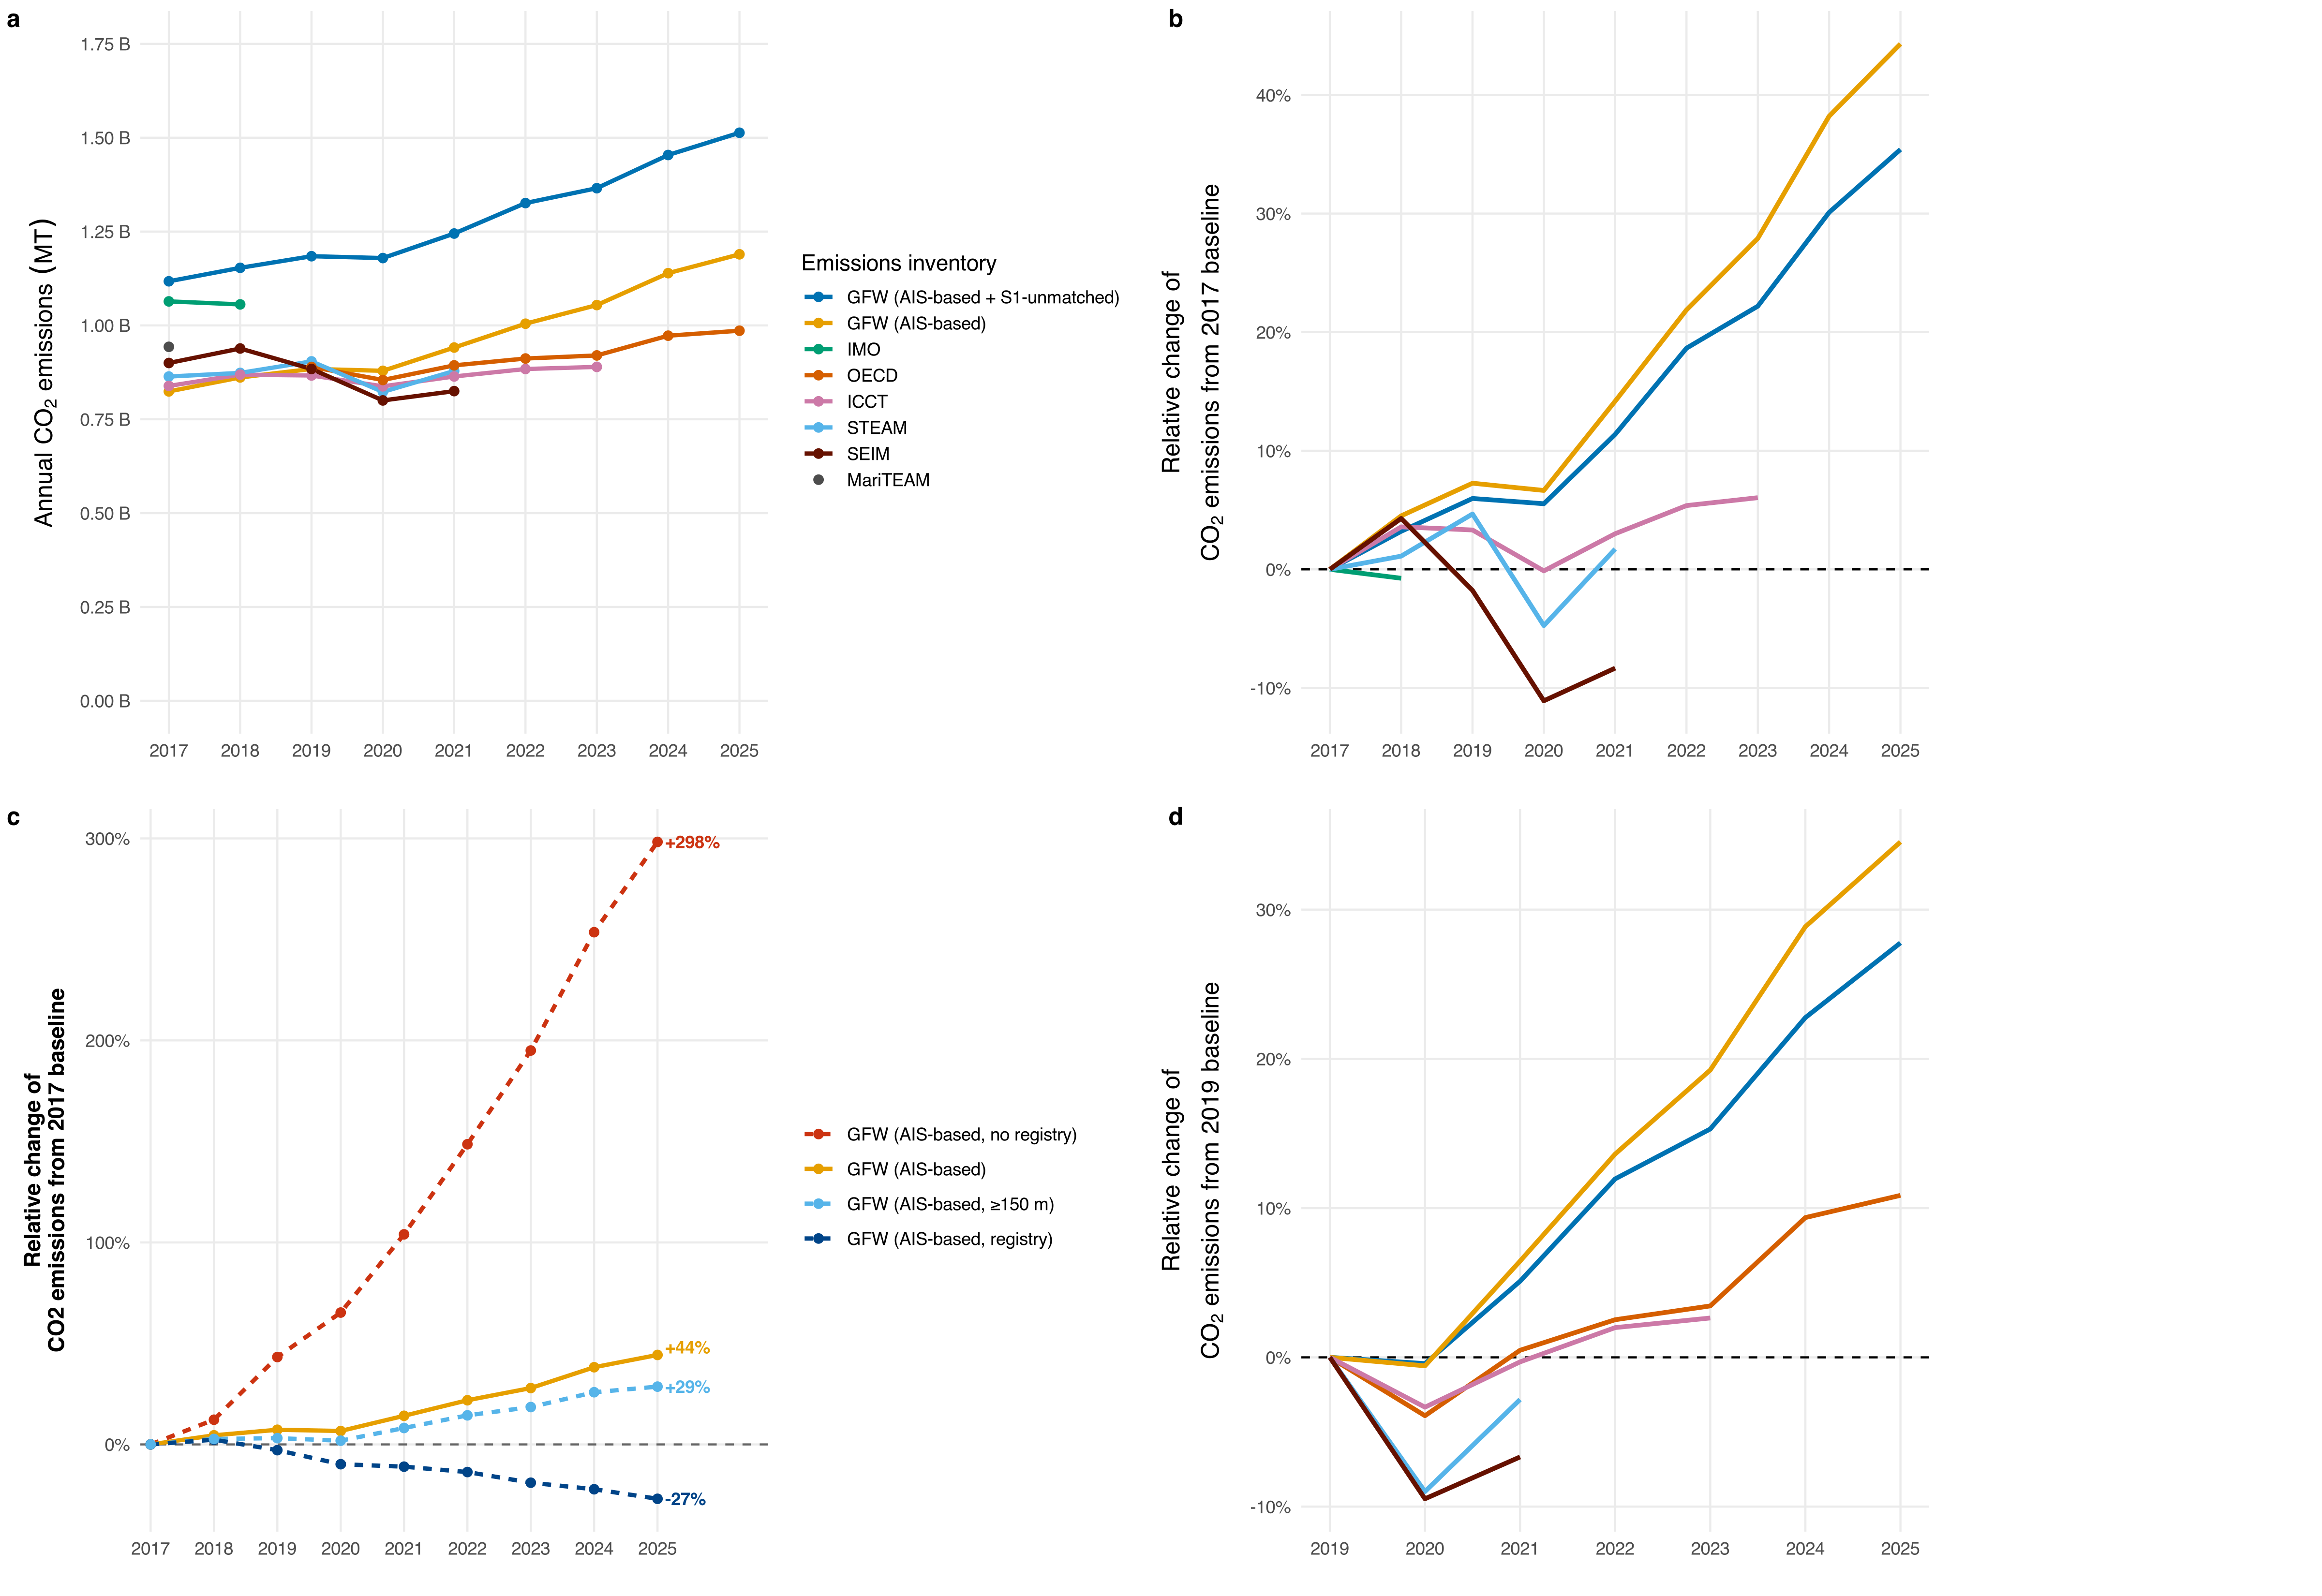
\includegraphics[width=\columnwidth]{figures/figS-inventory-comparison-all-sources-1.png}
    \caption{Trends in our AIS-based and fused estimates against other inventories. (a, b) Change relative to 2017 and to 2019, respectively, against the published bottom-up inventories; the 2019 baseline allows inclusion of OECD, whose series begins in 2019. (c) Change relative to 2017 against the top-down EDGAR and CEDS inventories, for shipping, all other transportation modes, and all sectors. (d) Our AIS-based series split by vessel length, relative to 2017, using the length bands of Supplementary Table \ref{tab:growth_share_by_family_length}.}
    \label{fig:figS-inventory-comparison-all-sources}
\end{figure}

% Nine columns overflow the text block at the default column padding
\begingroup
\setlength{\tabcolsep}{2.5pt}
\begin{table}[!h]
\centering
\caption{\label{tab:inventory_comparison_all_sources}Annual marine vessel CO$_{2}$ emissions (billions of metric tonnes) for our AIS-based and fused (AIS-based + S1-unmatched) estimates and for the published bottom-up, activity-based inventories. A dash marks a year for which an inventory publishes no estimate.}
\centering
\fontsize{7}{9}\selectfont
\setlength{\tabcolsep}{3pt}
\begin{tabular}[t]{r|l|l|l|l|l|l|l|l}
\hline
Year & \shortstack{GFW\\(AIS-based +\\S1-unmatched)} & \shortstack{GFW\\(AIS-based)} & IMO & OECD & SAVE (ICCT) & STEAM & SEIM & MariTEAM\\
\hline
2017 & 1.118 & 0.824 & 1.064 & - & 0.839 & 0.864 & 0.900 & 0.943\\
\hline
2018 & 1.153 & 0.861 & 1.056 & - & 0.869 & 0.874 & 0.939 & -\\
\hline
2019 & 1.184 & 0.884 & - & 0.889 & 0.867 & 0.904 & 0.884 & -\\
\hline
2020 & 1.179 & 0.879 & - & 0.855 & 0.838 & 0.823 & 0.800 & -\\
\hline
2021 & 1.245 & 0.941 & - & 0.894 & 0.864 & 0.879 & 0.825 & -\\
\hline
2022 & 1.326 & 1.005 & - & 0.912 & 0.884 & - & - & -\\
\hline
2023 & 1.366 & 1.054 & - & 0.920 & 0.890 & - & - & -\\
\hline
2024 & 1.454 & 1.139 & - & 0.973 & - & - & - & -\\
\hline
2025 & 1.513 & 1.189 & - & 0.986 & - & - & - & -\\
\hline
\end{tabular}
\end{table}

\endgroup
\FloatBarrier

In the most recent years our AIS-based series grows faster than every other inventory (Supplementary Fig. \ref{fig:figS-inventory-comparison-all-sources}, panels a and b). The difference lies in how the fleets are defined. Inventories constrained by commercial registries change primarily at the pace of registry updates and activity of vessels within the registry, whereas our fleet is defined by AIS observation and grows with AIS carriage. Our broadcasting fleet accordingly grows faster than the OECD and SAVE fleets, the only inventories publishing vessel counts over the recent period, and most of that growth comes from small vessels (Supplementary Table \ref{tab:growth_share_by_family_length}; Supplementary Fig. \ref{fig:figS-inventory-comparison-all-sources}, panel d; Supplementary Fig. \ref{fig:figS-growth-timeline-by-family-length}). Among detected large non-fishing vessels, the segment where AIS carriage is mandated and registry coverage is strongest, the share with no matching AIS broadcast is essentially unchanged since 2017, whereas it falls steeply among small non-fishing and fishing vessels as AIS carriage and reception expand (Supplementary Fig. \ref{fig:figS-ais-carriage-saturation-by-size}). Consistent with this, vessels under 50 m, which are numerous, largely coastal, and poorly covered by registries, contribute the largest share of the growth in our AIS-based series, led by passenger vessels (Supplementary Fig. \ref{fig:figS-passenger-size-panels}), and they enter it mainly as they begin to broadcast: of the 142 million tonne increase from service and passenger vessels under 50 m, 126 million tonnes came from the change in vessel count (Supplementary Table \ref{tab:growth_decomposition_by_family_length}). The phase-in of D-AIS (Supplementary Note \ref{sec:ais-receiver-types}) adds a second, smaller effect: AIS positions received more than doubled between 2021 and 2025 while observed distance traveled and AIS-based emissions rose together by only $\sim$27\%, so D-AIS mostly densified trajectories that were already observed rather than adding new activity. The exception is small fishing vessels: their distance per vessel rose 51\% between 2017 and 2025, accounting for 13 of their 35 million tonne increase, consistent with improved reception tracking vessels that were already broadcasting over more of their activity (Supplementary Table \ref{tab:growth_decomposition_by_family_length}). The divergence from the other inventories therefore suggests that the other inventories, and our own estimates for early years, miss part of the fleet, and that any AIS-based trend partly measures the expansion of AIS carriage rather than of activity at sea. We return to this second point below.

\begin{figure}[H]
    \centering
    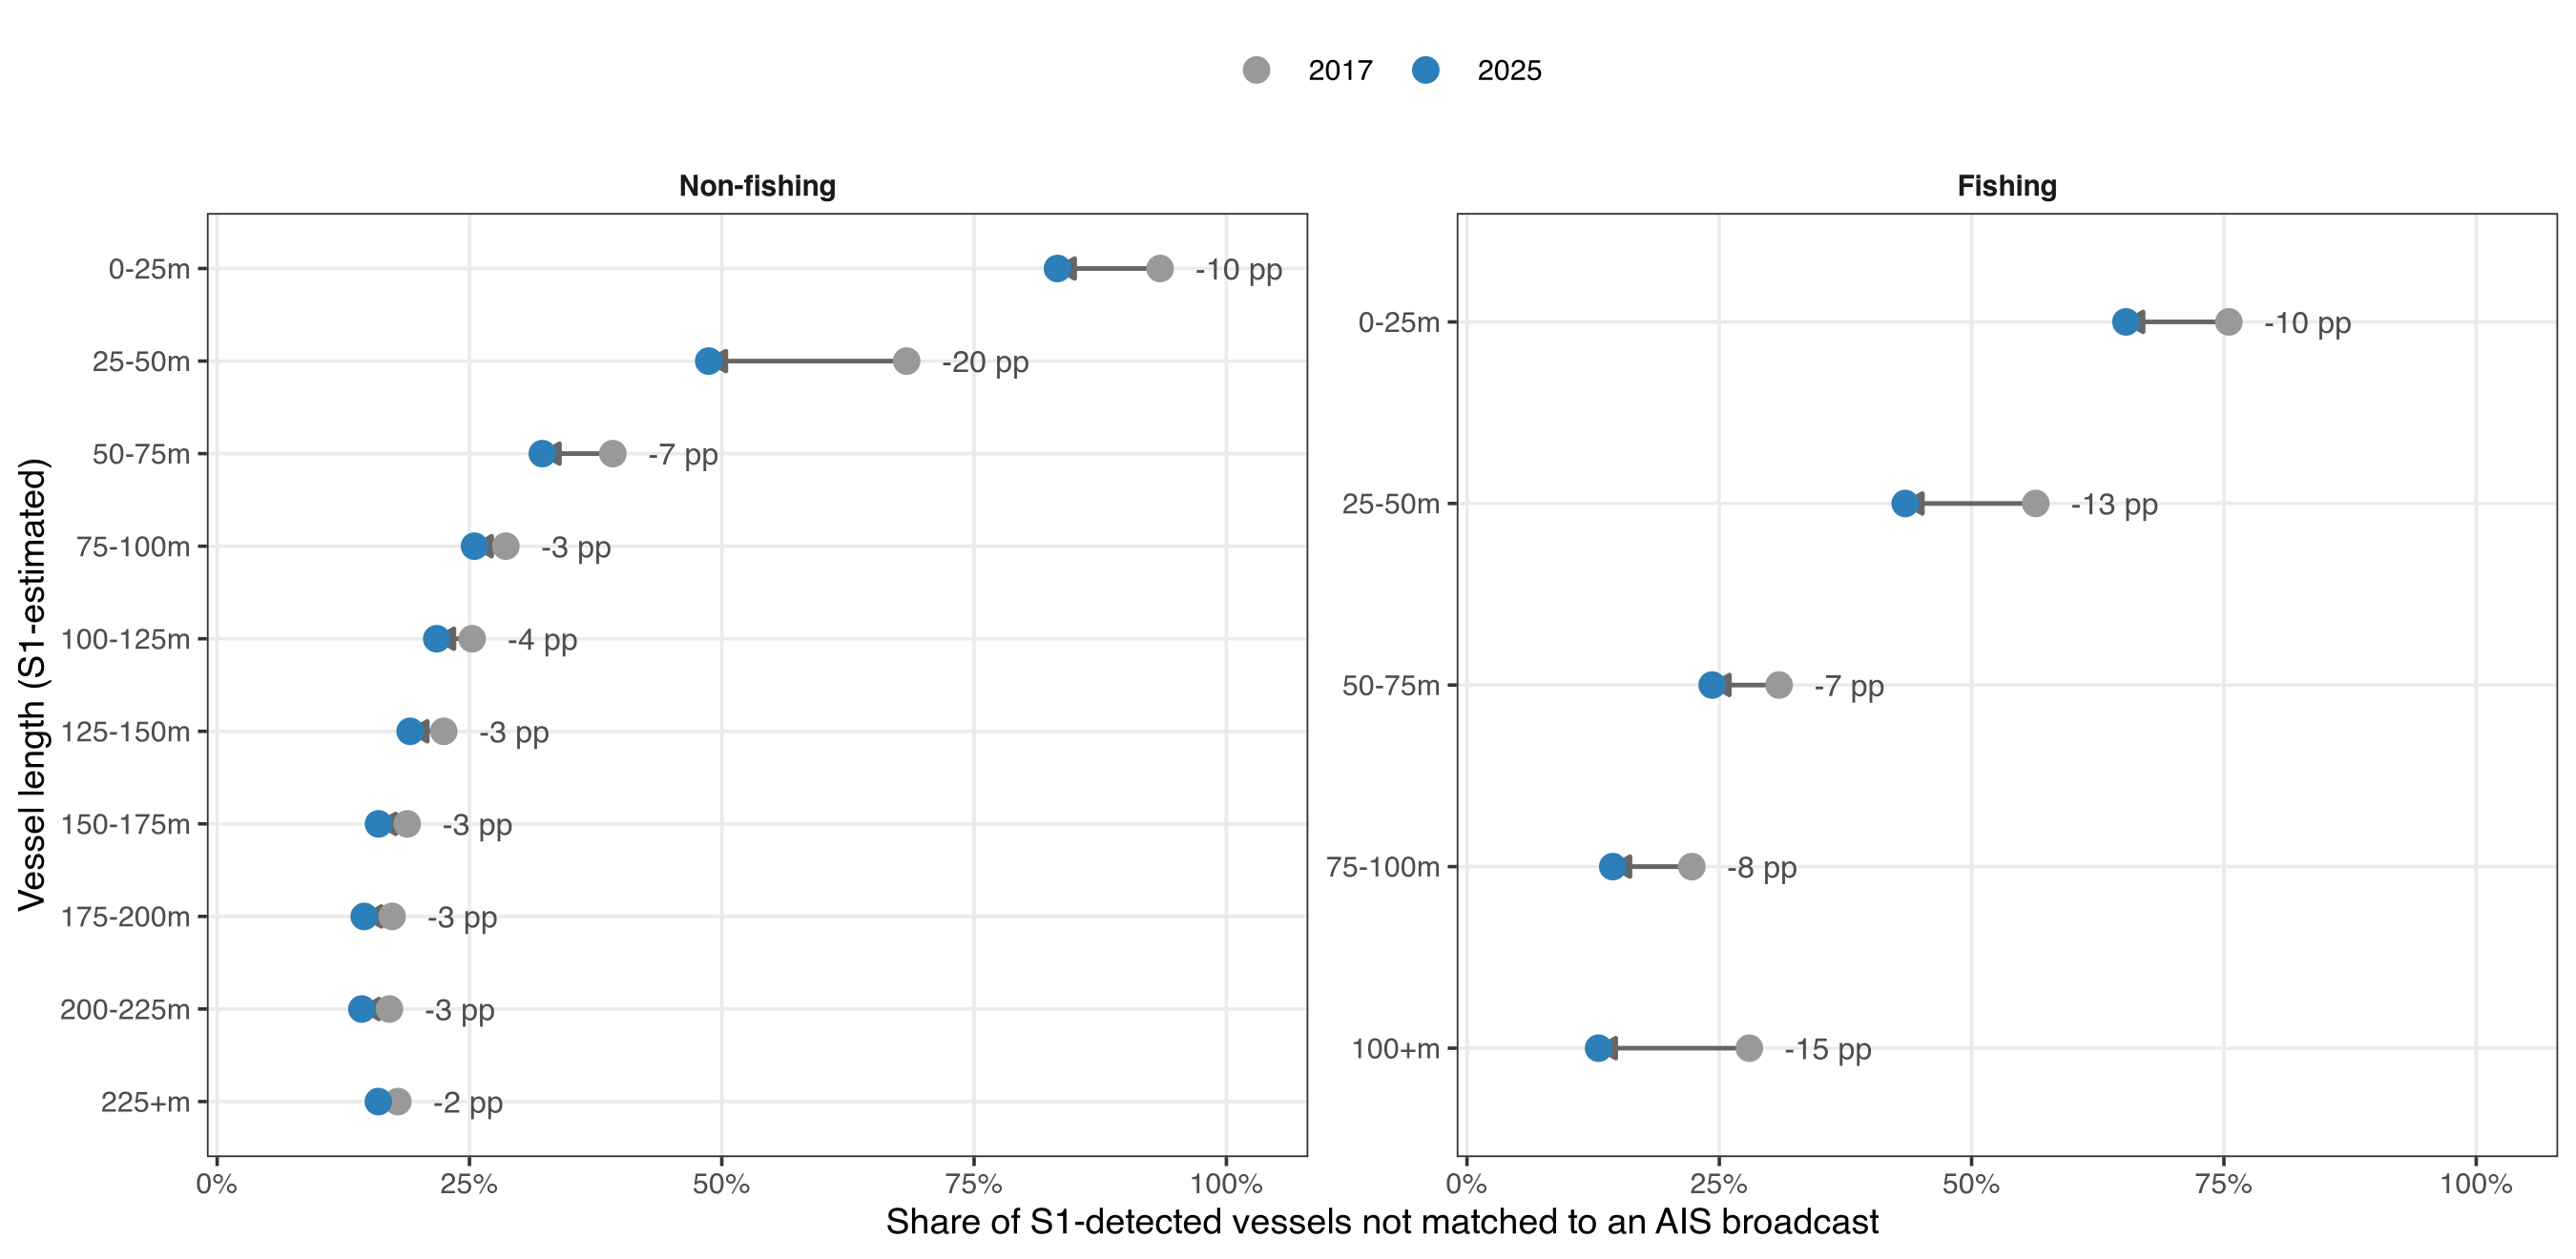
\includegraphics[width=\columnwidth]{figures/figS-ais-carriage-saturation-by-size-1.png}
    \caption{AIS carriage saturation by vessel size: share of S1 detections with no matching AIS broadcast, by length bin, 2017 against 2025. The unmatched share is flat for the largest vessels and falls steeply for the smallest.}
    \label{fig:figS-ais-carriage-saturation-by-size}
\end{figure}

Our fused total (AIS-based + S1-unmatched) exceeds every other inventory in every year after 2017 (Fig. \ref{fig:fig-emissions-inventory-comparison}, panel a) because it extends the fleet through satellite imagery-based detections to vessels that appear in neither registries nor AIS. The Fourth IMO GHG Study, OECD, and SAVE also attempt to account for non-broadcasting vessels by assigning small registered vessels without AIS signals the activity profiles of explicitly modeled vessels, yet only the IMO study approaches our total, because this imputation can only add vessels listed in a registry.

\subsubsection*{Comparing our estimates with top-down inventories}

We also compared our fused estimates against two inventories derived from fuel statistics, the Emissions Database for Global Atmospheric Research (EDGAR) and the Community Emissions Data System (CEDS). EDGAR builds its shipping estimate from reported fuel sales, representing international shipping from international marine bunkers and domestic activity from domestic navigation fuel statistics, with recent years extrapolated from Energy Institute fuel oil trends \cite{guizzardiGlobalUptoDate2025}; it can therefore only count fuel that was sold and reported. CEDS starts from the same fuel statistics but treats them as systematically under-reported and scales its global shipping total to bottom-up estimates, mainly the IMO GHG Studies \cite{hoeslyHistorical17502014Anthropogenic2018, ceds_data_and_assumptions}, so it also inherits the fleet-scope limits described above. Our fused total exceeds both (Fig. \ref{fig:fig-emissions-inventory-comparison}, panel b, tabulated in Supplementary Table \ref{tab:multisector_shipping_comparison}). The gap in magnitude and the gap in trend have different causes.

\begin{table}[!h]
\centering
\caption{\label{tab:multisector_shipping_comparison}Annual marine vessel CO$_{2}$ emissions (billions of metric tonnes) for our AIS-based and fused (AIS-based + S1-unmatched) estimates against the shipping sector of the top-down EDGAR and CEDS inventories, whose shipping scope combines international and domestic navigation. A dash marks a year for which an inventory publishes no estimate.}
\centering
\fontsize{8}{10}\selectfont
\begin{tabular}[t]{r|l|l|l|l}
\hline
Year & \shortstack{GFW\\(AIS-based +\\S1-unmatched)} & \shortstack{GFW\\(AIS-based)} & EDGAR - Shipping & CEDS - Shipping\\
\hline
2017 & 1.065 & 0.824 & 0.881 & 1.040\\
\hline
2018 & 1.098 & 0.861 & 0.887 & 1.031\\
\hline
2019 & 1.128 & 0.884 & 0.875 & 1.030\\
\hline
2020 & 1.122 & 0.879 & 0.798 & 0.937\\
\hline
2021 & 1.187 & 0.941 & 0.833 & 0.979\\
\hline
2022 & 1.259 & 1.005 & 0.837 & 0.975\\
\hline
2023 & 1.299 & 1.054 & 0.890 & 1.014\\
\hline
2024 & 1.384 & 1.139 & 0.860 & -\\
\hline
2025 & 1.443 & 1.189 & - & -\\
\hline
\end{tabular}
\end{table}

\FloatBarrier

\begin{table}[!h]
\centering
\caption{\label{tab:inventory_growth_comparison}Growth in CO$_2$ emissions for our estimates and for every inventory compared in Supplementary Note \ref{sec:inventory-comparison}. All series are anchored at 2017 where they extend that far back, and because the inventories end in different years each is summarized to its own end year. Growth is reported two ways: the total percent change between the first and last year, and the compound annual growth rate (CAGR). The Fourth IMO GHG Study ends in 2018 and is therefore reported over its native 2015-2018 window, since anchoring it at 2017 would leave a single year-on-year change. MariTEAM is a single-year inventory and admits no growth rate. EDGAR and CEDS changes are shown for All sectors, Other transportation and Shipping scopes.}
\centering
\fontsize{8}{10}\selectfont
\begin{tabular}[t]{l|c|r|r}
\hline
Series & Time window & Total \% change & CAGR (\%/yr)\\
\hline
\multicolumn{4}{l}{\textbf{Ours}}\\
\hline
\hspace{1em}GFW (AIS-based + S1-unmatched) & 2017--2025 & +35.41 & +3.86\\
\hline
\hspace{1em}GFW (AIS-based) & 2017--2025 & +44.31 & +4.69\\
\hline
\hspace{1em}GFW (AIS-based, $\geq$150 m) & 2017--2025 & +28.62 & +3.20\\
\hline
\multicolumn{4}{l}{\textbf{Bottom-up}}\\
\hline
\hspace{1em}IMO & 2015--2018 & +6.56 & +2.14\\
\hline
\hspace{1em}OECD & 2019--2025 & +10.85 & +1.73\\
\hline
\hspace{1em}SAVE & 2017--2023 & +6.04 & +0.98\\
\hline
\hspace{1em}STEAM & 2017--2021 & +1.71 & +0.42\\
\hline
\hspace{1em}SEIM & 2017--2021 & -8.33 & -2.15\\
\hline
\hspace{1em}MariTEAM & 2017 & --- & ---\\
\hline
\multicolumn{4}{l}{\textbf{EDGAR}}\\
\hline
\hspace{1em}All sectors & 2017--2024 & +7.06 & +0.98\\
\hline
\hspace{1em}Other transportation & 2017--2024 & +3.35 & +0.47\\
\hline
\hspace{1em}Shipping & 2017--2024 & -2.38 & -0.34\\
\hline
\multicolumn{4}{l}{\textbf{CEDS}}\\
\hline
\hspace{1em}All sectors & 2017--2023 & +5.60 & +0.91\\
\hline
\hspace{1em}Other transportation & 2017--2023 & +3.27 & +0.54\\
\hline
\hspace{1em}Shipping & 2017--2023 & -2.46 & -0.41\\
\hline
\end{tabular}
\end{table}

\FloatBarrier

The magnitude gap arises from three differences in the fleets these inventories can account for. First, fishing largely falls outside the shipping sector in both. They report fishing fuel combined with agriculture and forestry, so EDGAR's shipping estimate contains no fishing vessels at all, while in CEDS only some unreported fishing fuel is absorbed into global shipping through its scaling to bottom-up estimates. Second, small coastal and inland vessels are only partly covered: domestic navigation fuel is intended to capture this traffic, but the sector is inconsistently defined across reporting countries \cite{kuenen2014tno}. Third, neither inventory can capture fuel that never passes through reported channels, affecting vessels supplied informally or illegally. Each of these mechanisms adds emissions that the top-down inventories omit, and our own detection limits mean that we likely understate the total further.

Growth in our AIS-based series partly reflects expanding AIS carriage and coverage, as shown above. The fused total should be less sensitive to that: a vessel that adopts AIS and begins to broadcast moves from the S1-unmatched component to the AIS-based one, reallocating emissions between them rather than adding to the total. In principle, therefore, increases in the fused total should reflect new activity rather than changes in AIS coverage. S1 detections, which depend on neither AIS broadcasting nor registration, offer a partial check on that. Detected activity per observed area stayed roughly flat overall, but its composition shifted, growing among small non-fishing vessels and, most strongly, among the largest, while mid-size classes were flat and fishing declined (Supplementary Fig. \ref{fig:figS-density-by-match-status}, panel a). For the largest non-fishing vessels, AIS carriage is already near-universal and the unmatched share has barely changed since 2017 (Supplementary Fig. \ref{fig:figS-ais-carriage-saturation-by-size}), so their growth must largely reflect new activity; because a large vessel can emit on the order of a hundred times what a smaller one does, that compositional shift pushes the emissions trend upward.

\begin{figure}[H]
    \centering
    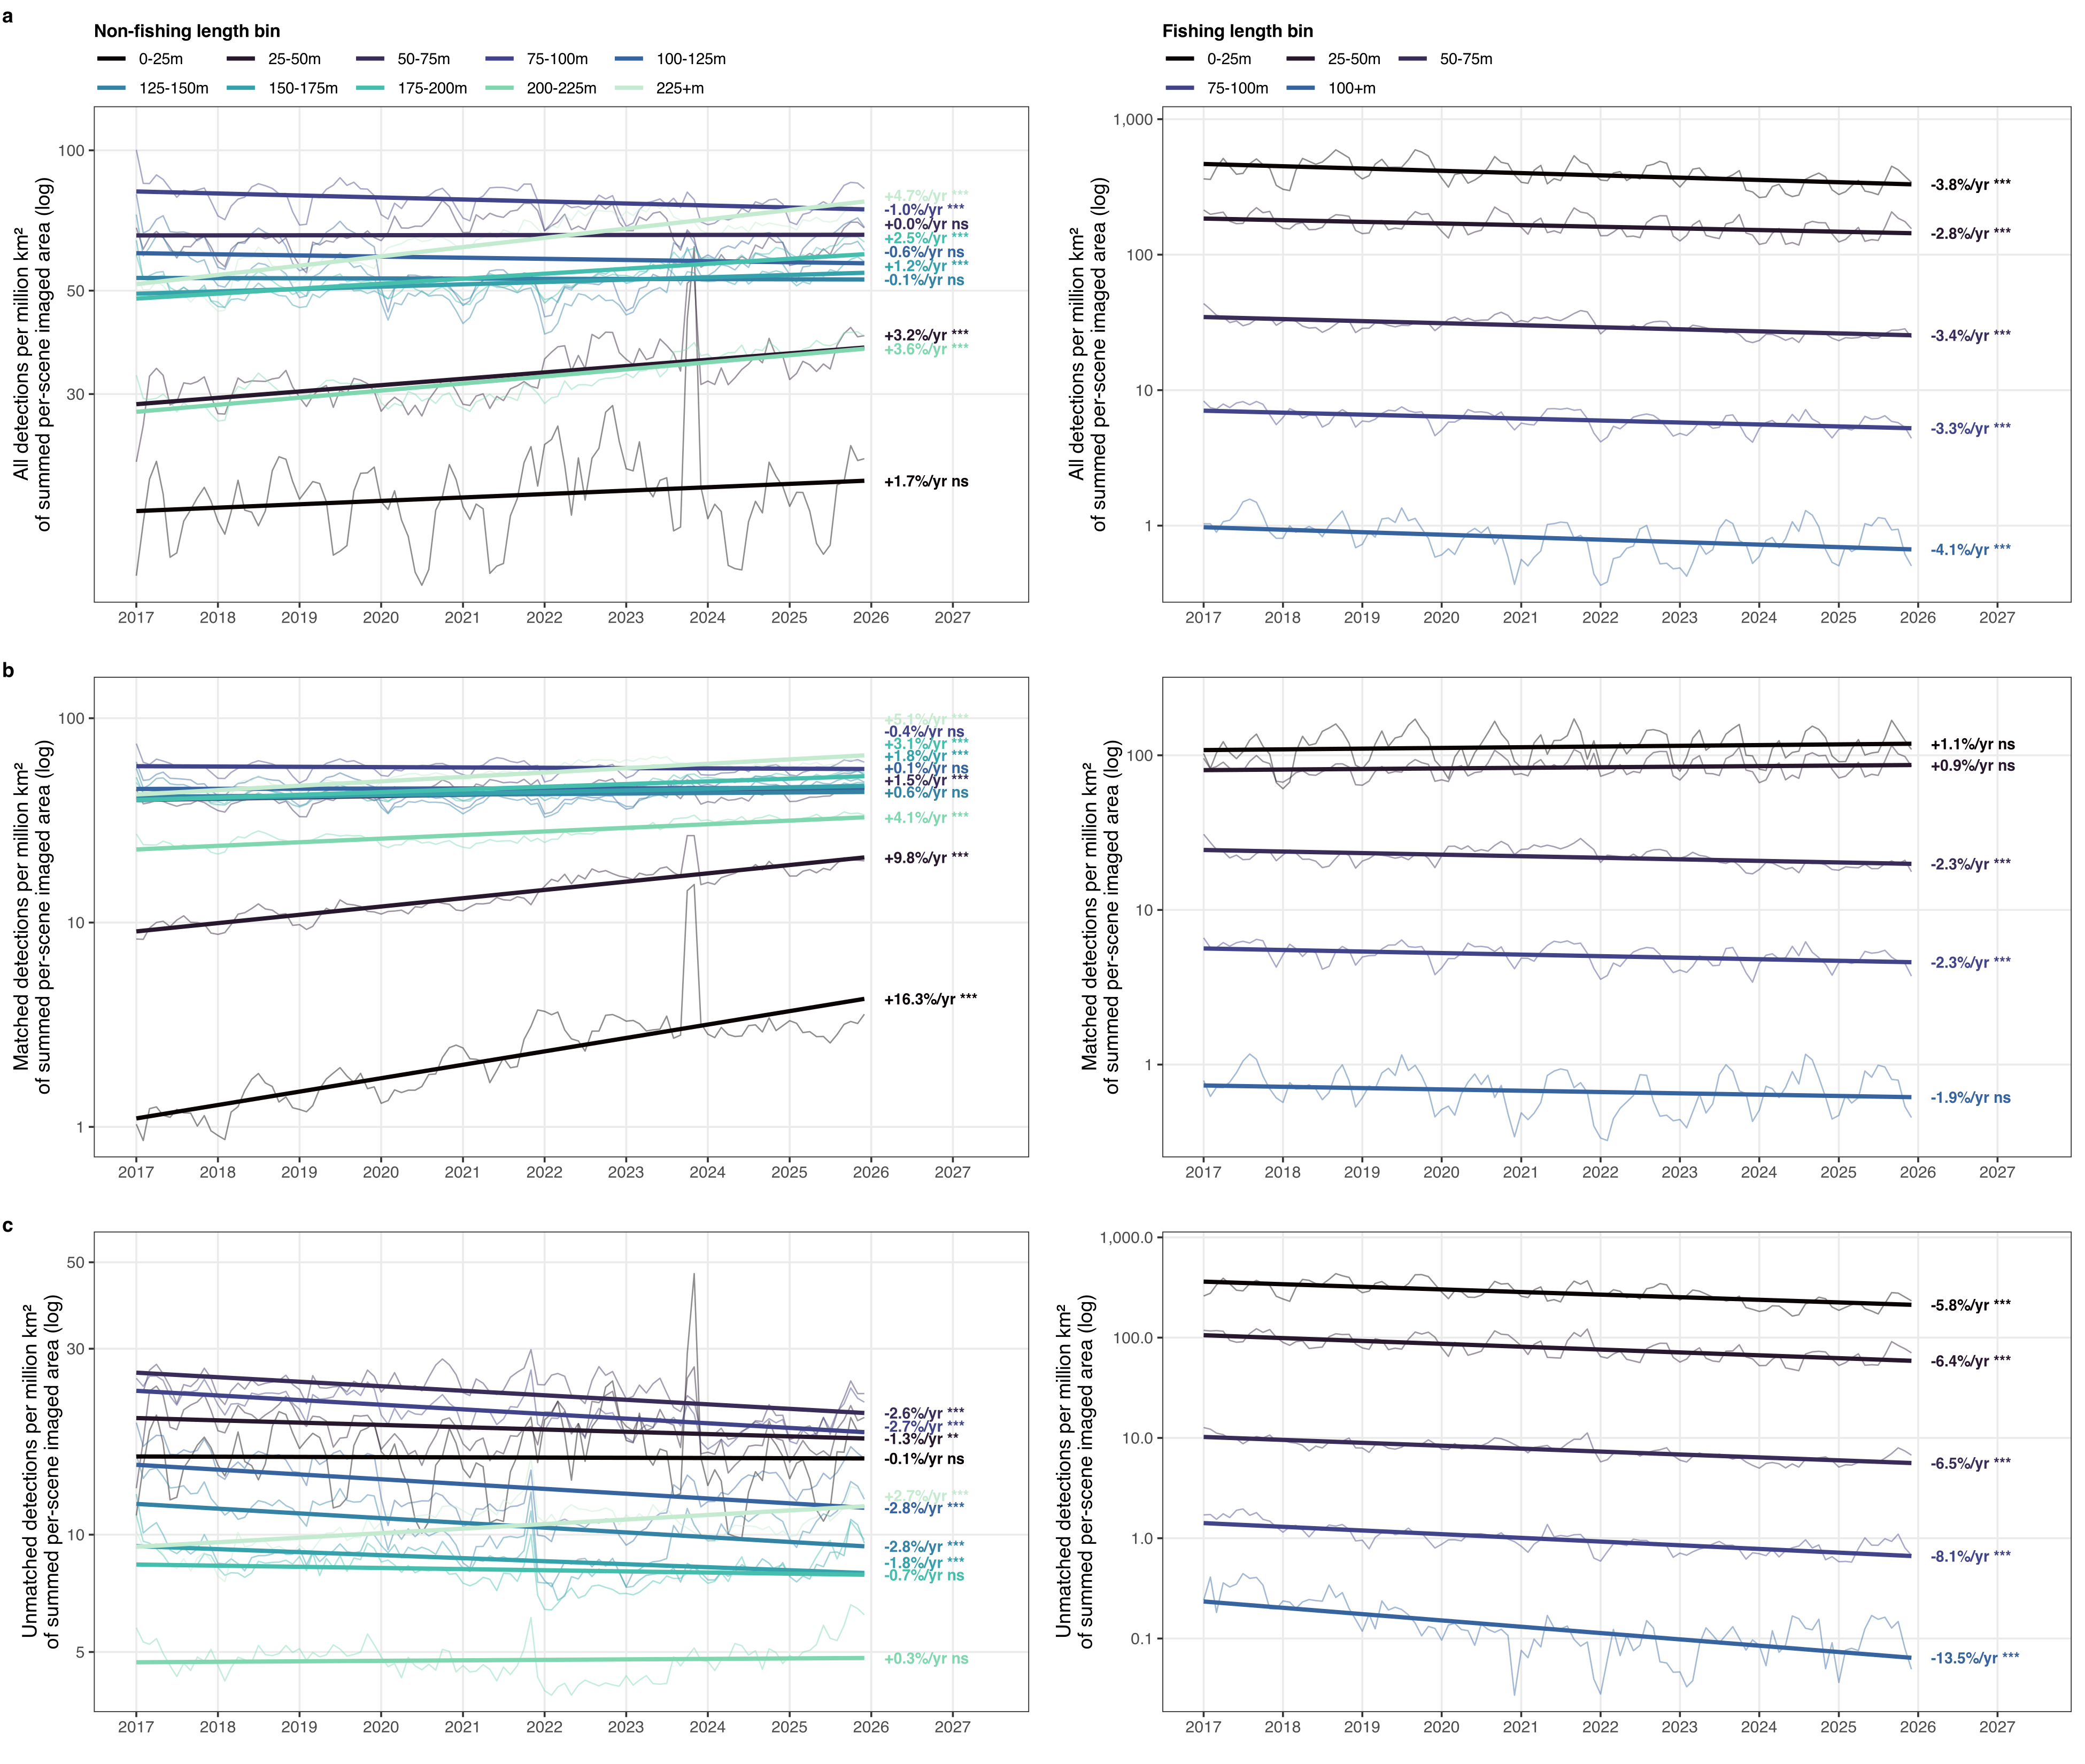
\includegraphics[width=\columnwidth]{figures/figS-density-by-match-status-1.png}
    \caption{S1 detection density by length bin, split into total, AIS-matched and unmatched detections, for fishing and non-fishing fleets, 2017--2025. Density is expressed per unit of S1 sampling effort on the same measure our emissions models use to normalize their detection features (detections per 10\textsuperscript{6} km² of per-scene imaged area summed across scenes), so the three series share a denominator and are additive. Axes are log scaled. Thin lines are monthly values; thick lines are ordinary least squares fits of log density on time over the full period, labeled with the fitted trend in percent change per year and its significance from the slope's two-sided $t$ test (*** $p<0.001$, ** $p<0.01$, * $p<0.05$, ns otherwise).}
    \label{fig:figS-density-by-match-status}
\end{figure}

Reallocation between our components, however, holds only where S1 had already detected the vessel. Vessels too small or too close to shore to be reliably detected contribute nothing to the S1-unmatched component and enter the fused total for the first time when they begin broadcasting. Because AIS carriage and reception expanded over the study period, that unobserved fraction was larger at the start of the series than at the end, so part of the measured growth in the fused total can be that gap closing rather than activity rising. The fact that our fused trend closely tracks the AIS-based trend, only slightly shallower at 36\% against 44\% growth between 2017 and 2025, is consistent with this: some reallocation and new activity occur, but part of the measured growth may enter directly through AIS adoption. This could bias our estimated growth trend upward relative to the true trend in activity, even in our fused estimates. However, this does not necessarily mean that the near-flat trends reported by other inventories are accurate either. A cleaner test comes from the part of the fleet our approach captures most completely, non-fishing vessels of 150 m and above, where AIS carriage was already saturated at the start of our series (Supplementary Fig. \ref{fig:figS-ais-carriage-saturation-by-size}). AIS-based emissions from this segment still rose 29\% between 2017 and 2025 (Supplementary Fig. \ref{fig:figS-inventory-comparison-all-sources}, panel d), and that growth came through the number of vessels rather than through distance per vessel, which is where improved reception would show (Supplementary Table \ref{tab:growth_decomposition_by_family_length}). S1-unmatched emissions are not disaggregated by vessel size, so we cannot give a fused figure for this segment separately. The growth that remains once observational expansion is set aside is thus lower than our headline figure, but still well above the near-flat trends of the other inventories: even confined to this segment of large non-fishing vessels, AIS-based emissions grew at a compound annual rate of 3.20\%, only 0.67 percentage points below the 3.87\% growth rate of our fused total emissions. This is still nearly twice that of OECD (1.73\%/yr), the fastest-growing bottom-up inventory that extends beyond 2018, more than three times that of global emissions across all sectors, and about six to seven times that of all other transportation modes combined (Supplementary Fig. \ref{fig:figS-inventory-comparison-all-sources}, Supplementary Table \ref{tab:inventory_growth_comparison}).
